% Options for packages loaded elsewhere
\PassOptionsToPackage{unicode}{hyperref}
\PassOptionsToPackage{hyphens}{url}
%
\documentclass[
]{book}
\usepackage{amsmath,amssymb}
\usepackage{iftex}
\ifPDFTeX
  \usepackage[T1]{fontenc}
  \usepackage[utf8]{inputenc}
  \usepackage{textcomp} % provide euro and other symbols
\else % if luatex or xetex
  \usepackage{unicode-math} % this also loads fontspec
  \defaultfontfeatures{Scale=MatchLowercase}
  \defaultfontfeatures[\rmfamily]{Ligatures=TeX,Scale=1}
\fi
\usepackage{lmodern}
\ifPDFTeX\else
  % xetex/luatex font selection
\fi
% Use upquote if available, for straight quotes in verbatim environments
\IfFileExists{upquote.sty}{\usepackage{upquote}}{}
\IfFileExists{microtype.sty}{% use microtype if available
  \usepackage[]{microtype}
  \UseMicrotypeSet[protrusion]{basicmath} % disable protrusion for tt fonts
}{}
\makeatletter
\@ifundefined{KOMAClassName}{% if non-KOMA class
  \IfFileExists{parskip.sty}{%
    \usepackage{parskip}
  }{% else
    \setlength{\parindent}{0pt}
    \setlength{\parskip}{6pt plus 2pt minus 1pt}}
}{% if KOMA class
  \KOMAoptions{parskip=half}}
\makeatother
\usepackage{xcolor}
\usepackage{longtable,booktabs,array}
\usepackage{calc} % for calculating minipage widths
% Correct order of tables after \paragraph or \subparagraph
\usepackage{etoolbox}
\makeatletter
\patchcmd\longtable{\par}{\if@noskipsec\mbox{}\fi\par}{}{}
\makeatother
% Allow footnotes in longtable head/foot
\IfFileExists{footnotehyper.sty}{\usepackage{footnotehyper}}{\usepackage{footnote}}
\makesavenoteenv{longtable}
\usepackage{graphicx}
\makeatletter
\def\maxwidth{\ifdim\Gin@nat@width>\linewidth\linewidth\else\Gin@nat@width\fi}
\def\maxheight{\ifdim\Gin@nat@height>\textheight\textheight\else\Gin@nat@height\fi}
\makeatother
% Scale images if necessary, so that they will not overflow the page
% margins by default, and it is still possible to overwrite the defaults
% using explicit options in \includegraphics[width, height, ...]{}
\setkeys{Gin}{width=\maxwidth,height=\maxheight,keepaspectratio}
% Set default figure placement to htbp
\makeatletter
\def\fps@figure{htbp}
\makeatother
\setlength{\emergencystretch}{3em} % prevent overfull lines
\providecommand{\tightlist}{%
  \setlength{\itemsep}{0pt}\setlength{\parskip}{0pt}}
\setcounter{secnumdepth}{5}
\usepackage{booktabs}
\ifLuaTeX
  \usepackage{selnolig}  % disable illegal ligatures
\fi
\usepackage[]{natbib}
\bibliographystyle{plainnat}
\IfFileExists{bookmark.sty}{\usepackage{bookmark}}{\usepackage{hyperref}}
\IfFileExists{xurl.sty}{\usepackage{xurl}}{} % add URL line breaks if available
\urlstyle{same}
\hypersetup{
  pdftitle={Artin's Algebra},
  pdfauthor={Ashan Jayamal},
  hidelinks,
  pdfcreator={LaTeX via pandoc}}

\title{Artin's Algebra}
\author{Ashan Jayamal}
\date{2024-04-06}

\usepackage{amsthm}
\newtheorem{theorem}{Theorem}[chapter]
\newtheorem{lemma}{Lemma}[chapter]
\newtheorem{corollary}{Corollary}[chapter]
\newtheorem{proposition}{Proposition}[chapter]
\newtheorem{conjecture}{Conjecture}[chapter]
\theoremstyle{definition}
\newtheorem{definition}{Definition}[chapter]
\theoremstyle{definition}
\newtheorem{example}{Example}[chapter]
\theoremstyle{definition}
\newtheorem{exercise}{Exercise}[chapter]
\theoremstyle{definition}
\newtheorem{hypothesis}{Hypothesis}[chapter]
\theoremstyle{remark}
\newtheorem*{remark}{Remark}
\newtheorem*{solution}{Solution}
\begin{document}
\maketitle

{
\setcounter{tocdepth}{1}
\tableofcontents
}
\hypertarget{matrices}{%
\chapter{Matrices}\label{matrices}}

\hypertarget{basic-operations}{%
\section{Basic Operations}\label{basic-operations}}

Let \(m\) and \(n\) be positive integers. An \(m \times n\) matrix is a collection of \(mn\) numbers arranged in a rectangular array.

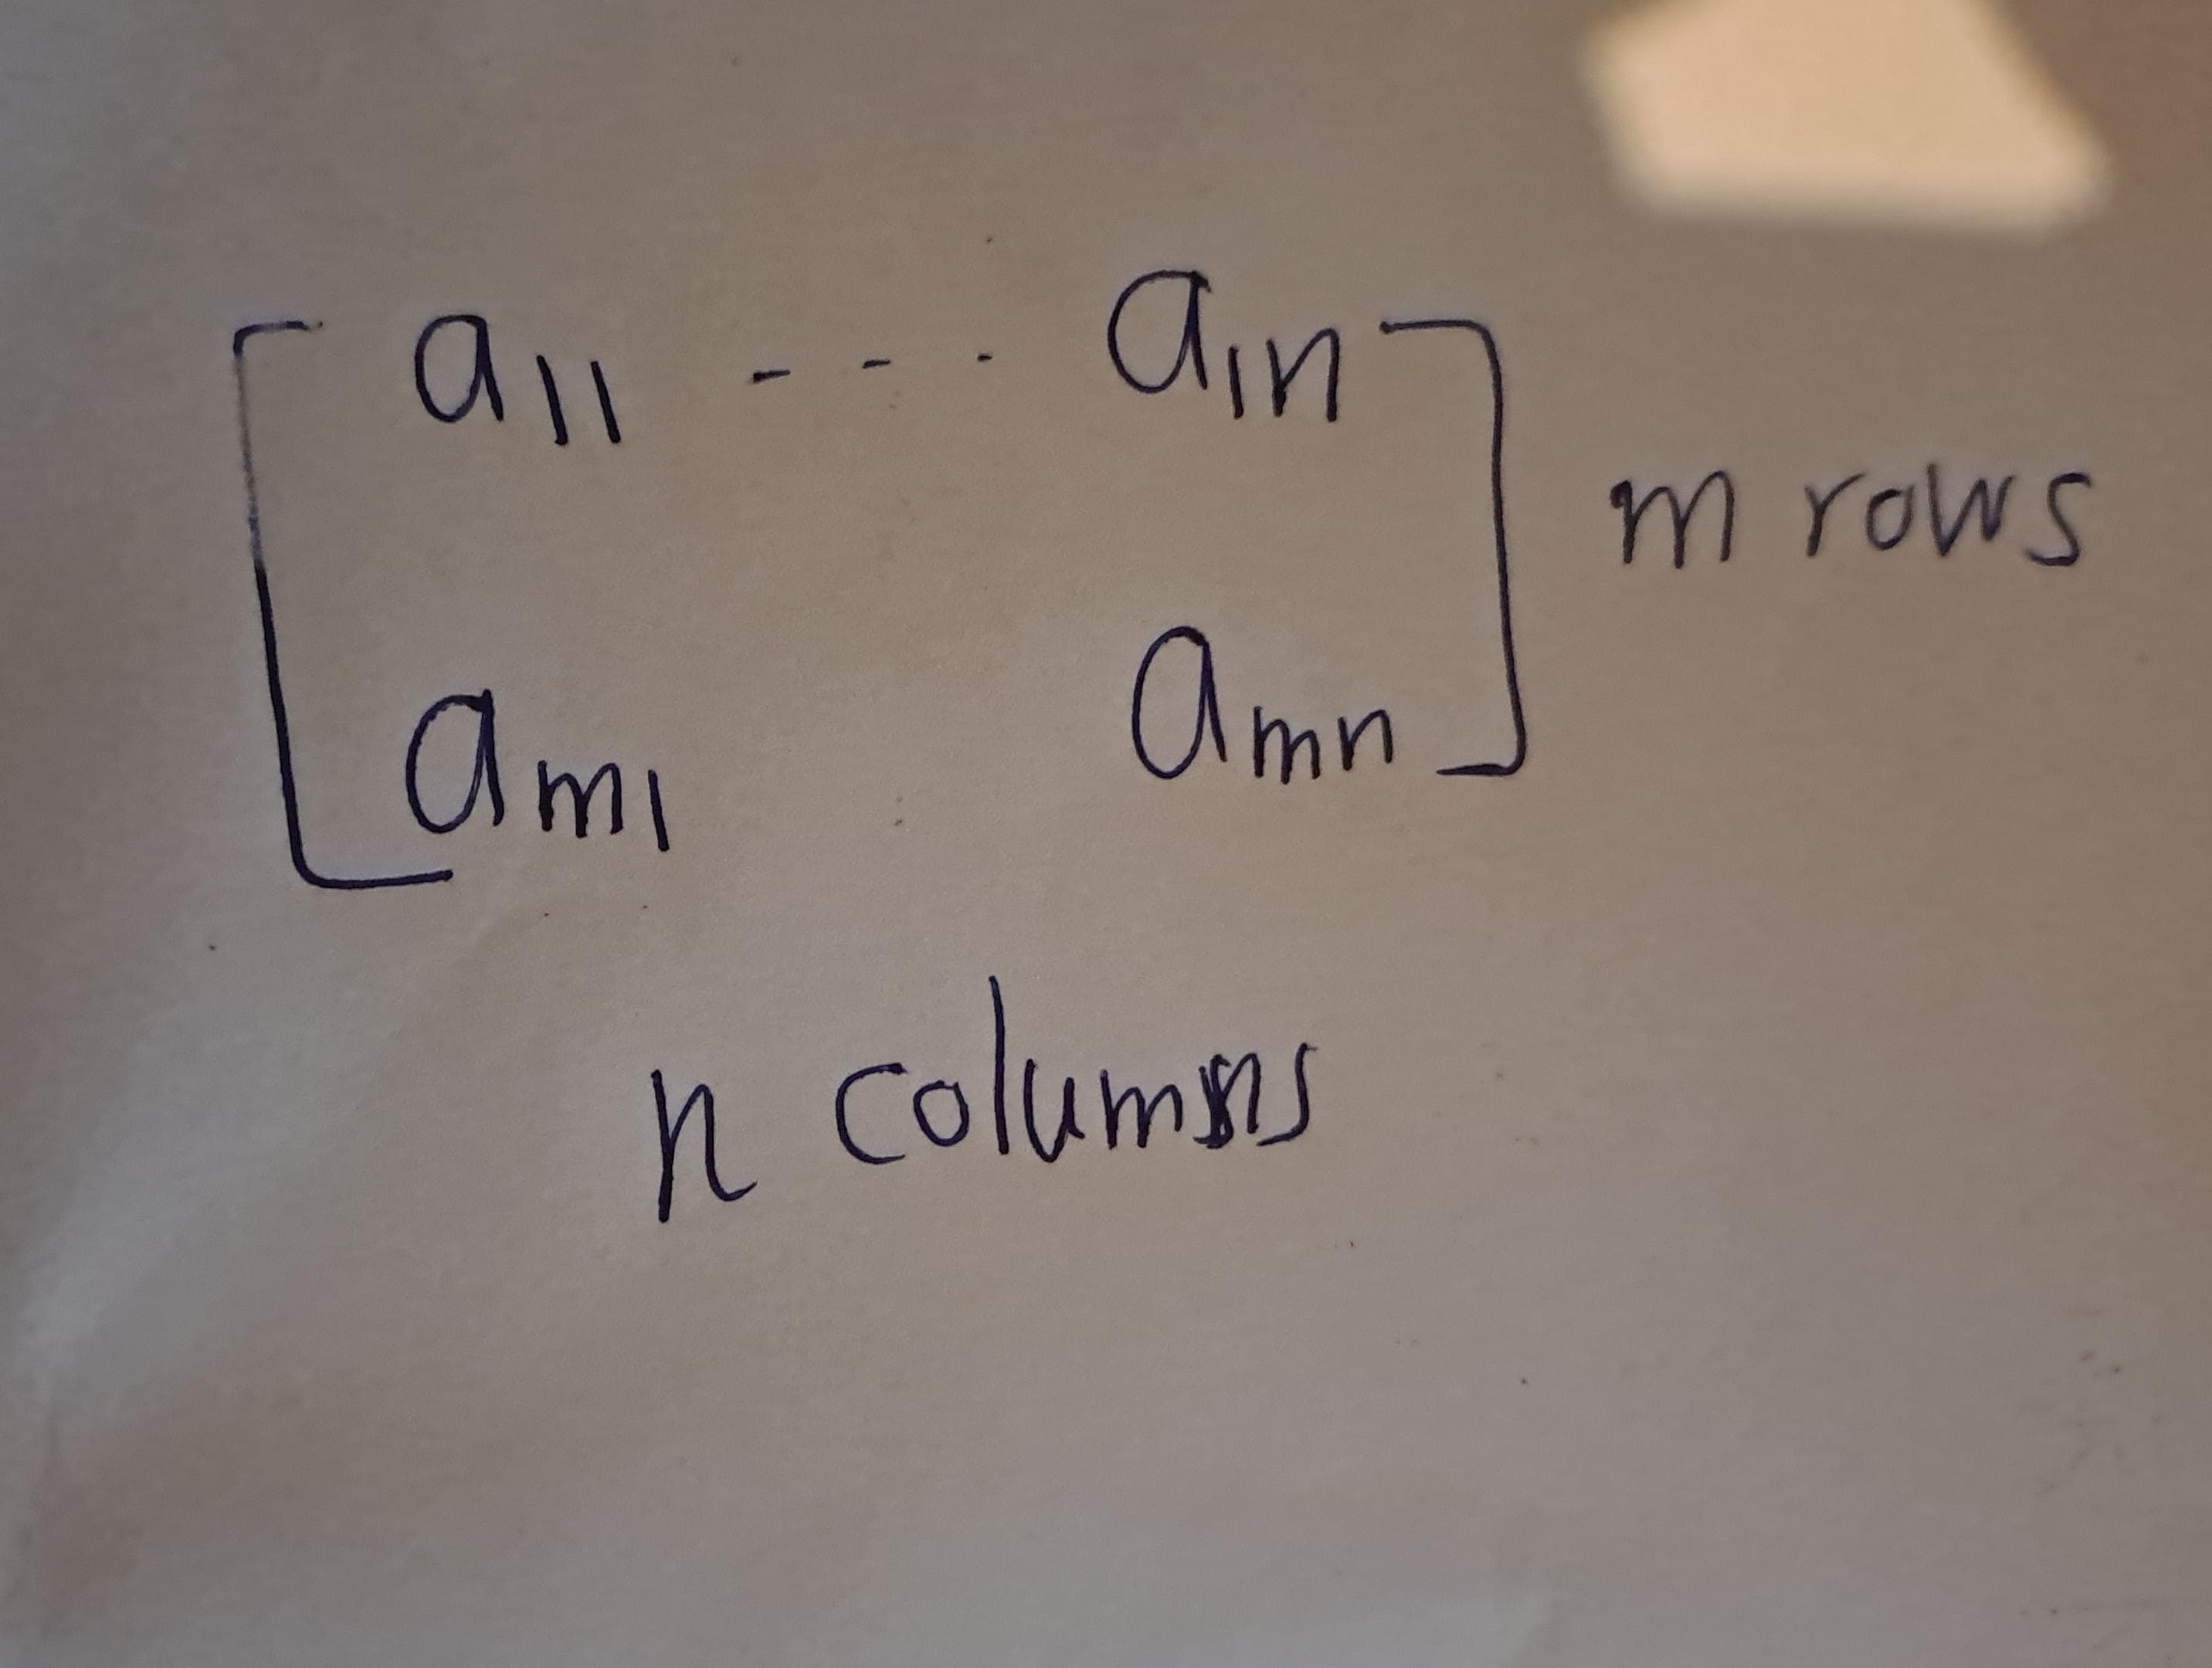
\includegraphics{figures/ch_1/fig01.jpg}
::: \{.example \#unnamed-chunk-1\}
\[A:=\begin{bmatrix}
8 & 0 & 3\\
78 & -5 & 2
\end{bmatrix}\]
\(A\) is \(2 \times 3\) matrix.(two rows and three columns)

:::
The numbers in a matrix are the matrix entries. They may be denoted by \(a_{ij}\), where \(i\) and \(j\) are indices (integers) with \(1 < i < m\) and \(1 < j < n\). The index \(i\) represents the row index, and \(j\) represents the column index. So \(a_{ij}\) is the entry that appears in the \(i\)th row and \(j\)th column of the matrix.

\begin{figure}
\centering
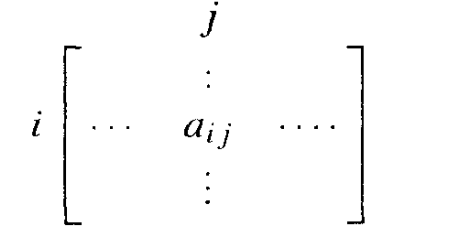
\includegraphics{figures/ch_1/fig02.png}
\caption{\label{fig:fig02}\(~\)}
\end{figure}

\hypertarget{group-theory}{%
\chapter{Group Theory}\label{group-theory}}

\hypertarget{laws-of-compositions}{%
\section{Laws of Compositions}\label{laws-of-compositions}}

\begin{definition}[Law of Composition]
\protect\hypertarget{def:unnamed-chunk-2}{}\label{def:unnamed-chunk-2}A law o f composition on a set \(S\) is any rule for combining pairs \(a, b\) of elements of \(S\) to get another element, say \(p\), of \(S\).
\end{definition}

\begin{example}
\protect\hypertarget{exm:unnamed-chunk-3}{}\label{exm:unnamed-chunk-3}\leavevmode

\begin{itemize}
\tightlist
\item
  Some models for this concept are addition and multiplication
  of real numbers.
\item
  Matrix multiplication on the set of \(n \times n\) matrices is another example.
\end{itemize}

\end{example}

Formally, a law of composition is a function of two variables, or a map,
\[S\times S \to S\]
Here, \(S \times S\) denotes, as always, the product set, whose elements are pairs \(a, b\) of elements of \(S\).

The element obtained by applying the law to a pair \(a, b\) is usually written using a notation resembling one used for multiplication or addition:
\[p = ab, a \times b, a \circ b, a + b\],
or whatever, a choice being made for the particular law in question. The element \(p\) may be called the product or the sum of a and b, depending on the notation chosen.

\hypertarget{groups-and-subgroups}{%
\section{Groups and Subgroups}\label{groups-and-subgroups}}

\begin{definition}[Group]
\protect\hypertarget{def:unnamed-chunk-4}{}\label{def:unnamed-chunk-4}

A group is a set \(G\) together with a law of composition that has the following properties:

\begin{itemize}
\tightlist
\item
  The law of composition is associative: \((ab)c = a(bc)\) for all \(a\), \(b\), \(c\) in \(G\).
\item
  \(G\) contains an identity element \(1\), such that \(la = a\) and \(al = a\) for all \(a\) in \(G\).
\item
  Every element \(a\) of \(G\) has an inverse, an element \(b\) such that \(ab = 1\) and \(ba = 1\).
\end{itemize}

\end{definition}

\textbf{Notation}: If set \(G\) with composition \(\cdot\) is a group, then we denote it by \((G,\cdot)\)
::: \{.definition \#unnamed-chunk-5 name=``Ableian Group''\}
Group G is called abliean if its law of composition is commutative. i.e.
\[\forall x\in G, xy=yx\]
:::

\begin{example}
\protect\hypertarget{exm:unnamed-chunk-6}{}\label{exm:unnamed-chunk-6}\leavevmode

\begin{itemize}
\tightlist
\item
  \(\mathbb{R}^\times:=\mathbb{R}\setminus \{0\}\) is an abliean group under multiplication
\item
  \(GL_n(\mathbb{R}):=\{A\in M_n(\mathbb{R}): \text{ A is invertible}\}\) with materix multiplication is non-abliean group. This group is called \emph{general linear group}.
\end{itemize}

\end{example}

\begin{definition}[Order of group]
\protect\hypertarget{def:unnamed-chunk-7}{}\label{def:unnamed-chunk-7}The order of a group \(G\) is the number of elements that it contains. We \[| G | := \text{number of elements of }G=\text{ the order of G}\]

If the order is finite, \(G\) is said to be a finite group. If not, \(G\) is an infinite group.
\end{definition}

Here is our notation for some familiar infinite abelian groups:

\begin{example}
\protect\hypertarget{exm:unnamed-chunk-8}{}\label{exm:unnamed-chunk-8}\leavevmode

\begin{itemize}
\tightlist
\item
  \((\mathbb{Z},+)\) :The set of integers, with addition as itslaw of composition (the additive group of integers)
\item
  \((\mathbb{R},+)\) :The set of real numbers, with addition as its law of
  composition (the additive group of real numbers)
\item
  \((\mathbb{R}^\times,\times)\) :The set of nonzero real numbers, with multiplication as its law of composition(the multiplicative group)
  \((\mathbb{C},+)\) :the set of complex numbers, with addition as its law of composition (the additive group of complex numbers)
\item
  \((\mathbb{C}^\times,\times)\) :The set of nonzero complex numbers, with multiplication as its law of composition(the multiplicative group of complex numbers)
\end{itemize}

\end{example}

\begin{proposition}[Cancellation Law]
\protect\hypertarget{prp:unnamed-chunk-9}{}\label{prp:unnamed-chunk-9}

Let \(G\) be group and let \(a, b, c \in G\) whose law of composition is written multiplicatively.

\begin{itemize}
\tightlist
\item
  If \(ab = ac\) or if \(ba = ca\), then \(b = c\).
\item
  If \(a b = a\) or if \(ba = a\), then \(b = 1\)
\end{itemize}

\end{proposition}

\begin{proof}
Multiply both sides of \(ab=ac\) on the left by\(a^{-1}\) to obtain \(b = c\). The other proofs are analogous.
\end{proof}

\begin{remark}
As you saw \(a^{-1}\) plays amajor rule in above proof. So the cancelation rule does not holds when elemenet \(a\) is not invertible.
\end{remark}

\begin{example}[Example that not holding the cancelation law]
\protect\hypertarget{exm:unnamed-chunk-12}{}\label{exm:unnamed-chunk-12}\[\begin{bmatrix} 1 & 1 \\ 0 & 0\end{bmatrix}
\begin{bmatrix} 1 & 1 \\ 2 & 0\end{bmatrix}=
\begin{bmatrix} 1 & 1 \\ 0 & 0\end{bmatrix}
\begin{bmatrix} 3 & 0 \\ 0 & 1\end{bmatrix}\]
\end{example}

\begin{example}
\protect\hypertarget{exm:unnamed-chunk-13}{}\label{exm:unnamed-chunk-13}Let \(T\) be a set and \(G:=\{f:T\to T: f \text{ is a bijection}\}\). Then \(G\) with composition is a group. We use notation \$sys(T) \$ to denote the
\end{example}

\begin{example}
\protect\hypertarget{exm:unnamed-chunk-14}{}\label{exm:unnamed-chunk-14}

The group of permutations of the set of indices \(\{l, 2, ... , n\}\) is called the \emph{symmetric group},and is denoted by \(S_n\). Then \(|S_n|=n !\). So, \(S_n\) is a finite group of order \(n!\).

Let's disscuss some individualcases for n.

\begin{itemize}
\tightlist
\item
  \textbf{\(n=2\)}\\
  The permutations of a set \(\{1, 2\}\) of two elements are the identity \(i\) and the transposition \(\tau=(12)\).
  \[S_2:=\{id,(12)\}\]
\end{itemize}

\begin{longtable}[]{@{}lll@{}}
\toprule\noalign{}
\(\circ\) & \(id\) & \((12)\) \\
\midrule\noalign{}
\endhead
\bottomrule\noalign{}
\endlastfoot
\(id\) & \(id\) & \((12)\) \\
\((12)\) & \((12)\) & \(id\) \\
------ & ------ & ----- \\
\end{longtable}

\begin{itemize}
\tightlist
\item
  \(n=3\)\\
  \(S_3\) has order \(3!=6\). \(S_3\) serves as a convenient example because it is the smallest group whose law of composition isn't commutative. We will refer to it often. To describe it, we pick two particular permutations in terms of which we can write all others. We take the cyclic permutation \((123)\), and the transposition \((12)\), and label them as \(x\) and \(y\), respectively.Then
  \begin{eqnarray}
  x^3 &=& (123)^3=(123)(123)(123)=(123)(132)=id\\
  y^2 &=& (12)^2=(12)(12)=id\\
  yx  &=& (12)(123)=(13)=(132)(12)=((123)(123))(12)=(123)^2(12)
  \end{eqnarray}
  As a summary,
  \[x^3=1,Y^2=1,yx=x^2y\]
\end{itemize}

\end{example}

\hypertarget{subgroups-of-the-additive-group-of-integers}{%
\section{Subgroups of the Additive Group of Integers}\label{subgroups-of-the-additive-group-of-integers}}

We review some elementary number theory here, in terms of subgroups of the additive group \(\mathbb{Z}^+\) of integers. To begin, we list the axioms for a subgroup when additive notation is used in the group: A subset \(S\) of a group \(G\) with law of composition written additively is a subgroup if it has these properties:

\begin{itemize}
\tightlist
\item
  \emph{Closure} : If \(a\) and \(b\) are in \(S\), then \(a + b\) is in \(S\).
\item
  \emph{Identity} : \(0\) is in \(S\).
\item
  \emph{Inverses} : If \(a\) is in \(S\) then \(-a\) is in \(S\).
\end{itemize}

Let \(a\) be an integer different from \(O\).
We denote the subset of \(\mathbb{Z}\) that consists of all
multiples of \(a\) by \(a\mathbb{Z}\):
\[a\mathbb{Z} := \{n \in \mathbb{ Z} | n = ka \text{ for some } k\in \mathbb{Z}\} \].

This is a subgroup of \(\mathbb{Z}^+\). Its elements can also be described as the integers divisible by \(a\).

\begin{theorem}
\protect\hypertarget{thm:unnamed-chunk-15}{}\label{thm:unnamed-chunk-15}Let \(S\) be a subgroup of the additive group \(\mathbb{Z}^+\). Either \(S\) is the trivial subgroup
\(\{0\}\), or else it has the form \(a\mathbb{Z}\), where \(a\) is the smallest positive integer in \(S\).
\end{theorem}

\begin{proof}
Let \(S\) be a subgroup of \(\mathbb{Z}^+\). Then \(0\in S\), and if \(0\) is the only element of \(S\) then \(S\) is the trivial subgroup. ie.: \(S=\{0\}\)So that case is settled.

Otherwise, \(S\) contains an integer \(n\) different from \(0\), and either \(n\) or \(-n\) is positive. The third property of a subgroup tells us that \(-n\) is in \(S\), so in either case, \(S\) contains a positive integer. We must show that \(S\) is equal to \(a\mathbb{Z}\), when \(a\) is the smallest positive integer in \(S\).

We first show that \(a\mathbb{Z}\) is a subset of \(S\), in other words, that \(ka\) is in \(S\) for every integer \(k\). If \(k\) is a positive integer, then \(ka = a + a + \cdots + a\) (\(k\) terms). Since \(a\) is in \(S\), closure and induction show that \(ka\) is in \(S\). Since inverses are in \(S\), \(-ka\) is in \(S\). Finally, \(0 = 0a\) is in \(S\).

Next we show that \(S\) is a subset of \(Za\), that is, every element \(n\) of \(S\) is an integer multiple of \(a\). We use division with remainder to write \(n = qa + r\), where \(q\) and \(r\) are integers and where the remainder \(r\) is in the range \(0 < r < a\). Since \(Za\) is contained in \(S\), \(qa\) is in \(S\), and of course \(n\) is in \(S\). Since \(S\) is a subgroup, \(r = n - qa\) is in \(S\) too. Now by our choice, \(a\) is the smallest positive integer in \(S\), while the remainder \(r\) is in the range \(0 < r < a\). The only remainder that can be in \(S\) is \(0\). So \(r = 0\) and \(n\) is the integer multiple \(qa\) of \(a\).
\end{proof}

\hypertarget{cyclic-groups}{%
\section{Cyclic Groups}\label{cyclic-groups}}

\hypertarget{homomorphisms}{%
\section{Homomorphisms}\label{homomorphisms}}

\begin{definition}
\protect\hypertarget{def:unnamed-chunk-17}{}\label{def:unnamed-chunk-17}Let \((G, *)\) and \((G', \odot)\) be groups. A \textbf{homomorphism} \(\phi: G \rightarrow G'\) is a map from \(G\) to \(G'\) such that for all \(a\) and \(b\) in \(G\):

\begin{equation}
    \phi(a * b) = \phi(a) \odot \phi(b).
\end{equation}
\end{definition}

\textbf{Examples of Homomorphisms}

\begin{enumerate}
\def\labelenumi{\arabic{enumi}.}
\tightlist
\item
  \textbf{Determinant Function}: \(\text{det}: GL_n(\mathbb{R}) \to \mathbb{R}^\times\)
\item
  \textbf{Exponential Map}: \(\text{exp}: (\mathbb{R}, +) \to (\mathbb{R}^\times, \times)\) defined by \(x \mapsto e^x\)
\item
  \textbf{Map \(\phi\)}: \((\mathbb{Z}, +) \to G\) defined by \(\phi(n) = a^n\), where \(a\) is a given element of \(G\)
\item
  \textbf{Absolute Value Map}: \(|\cdot| : (\mathbb{C}^\times, \times) \to (\mathbb{R}^\times, \times)\)
\end{enumerate}

\textbf{Trivial Homomorphism}

The trivial homomorphism \(\phi: G \rightarrow G'\) between any two groups maps every element of \(G\) to the identity in \(G'\).

\textbf{Inclusion Map}

If \(H\) is a subgroup of \(G\), the inclusion map \(i: H \rightarrow G\) defined by \(i(x) = x\) for \(x\) in \(H\) is a homomorphism.

\begin{proposition}
\protect\hypertarget{prp:unnamed-chunk-18}{}\label{prp:unnamed-chunk-18}

Let \(\phi: G \rightarrow G'\) be a group homomorphism.

\begin{enumerate}
\def\labelenumi{(\alph{enumi})}
\item
  If \(a_i, \ldots, a_k\) are elements of \(G\), then \(\phi(a_i \ldots a_k) = \phi(a_i) \ldots \phi(a_k)\).
\item
  \(\phi\) maps the identity to the identity: \(\phi(1_G) = 1_{G'}\).
\item
  \(\phi\) maps inverses to inverses: \(\phi(a^{-1}) = \phi(a)^{-1}\).
\end{enumerate}

\end{proposition}

\begin{proposition}
\protect\hypertarget{prp:258}{}\label{prp:258}

Let \(\phi : G \rightarrow G'\) be a homomorphism of groups, and
let \(a,b\in G\). Let \(K\ker(\phi)\).
Then following conditions are equivalent:

\begin{itemize}
\tightlist
\item
  \(\phi(a) = \phi(b)\),\\
\item
  \(a^{-1}b\) is in \(K\),
\item
  \(b\) is in the coset \(aK\),
\item
  The cosets \(bK\) and \(aK\) are equal.
\end{itemize}

\end{proposition}

\begin{proof}
\leavevmode

\begin{itemize}
\tightlist
\item
  \((1)\implies (2)\).\textbackslash{}
  Suppose \(\phi(a) = \phi(b)\). Now consider
  \[\phi(a^{-1}b)=\phi(a^{-1})\phi(b)=\phi(a^{-1} )\phi(b)=1\]
  Thus, \(a^{-1}b\in K\).
\item
  \((2)\implies (1)\)\textbackslash{} If \(a^{-1}b \in K\)
  \[1=\phi(a^{-1}b)=\phi(a^{-1})\phi(b)=\phi(a^{-1} )\phi(b)\].
  Thus, \(\phi(a)=\phi(b)\).
  \((3) \implies (4)\)
\item
  Suppose \(b\) is in the coset \(aK\). Then \(b=ak\) for some
\end{itemize}

\end{proof}

\hypertarget{isomorphisms}{%
\section{Isomorphisms}\label{isomorphisms}}

\hypertarget{equivalence-relations-and-partitions}{%
\section{Equivalence Relations and Partitions}\label{equivalence-relations-and-partitions}}

\begin{definition}
\protect\hypertarget{def:unnamed-chunk-20}{}\label{def:unnamed-chunk-20}Sure, here is the LaTeX version of your statement:

A partition \(n\) of a set \(S\) is a subdivision of \(S\) into nonoverlapping, nonempty subsets:
\[S = \bigcup_{i} A_i\]
,where \(A_i\) are disjoint nonempty subsets of \(S\).
\end{definition}

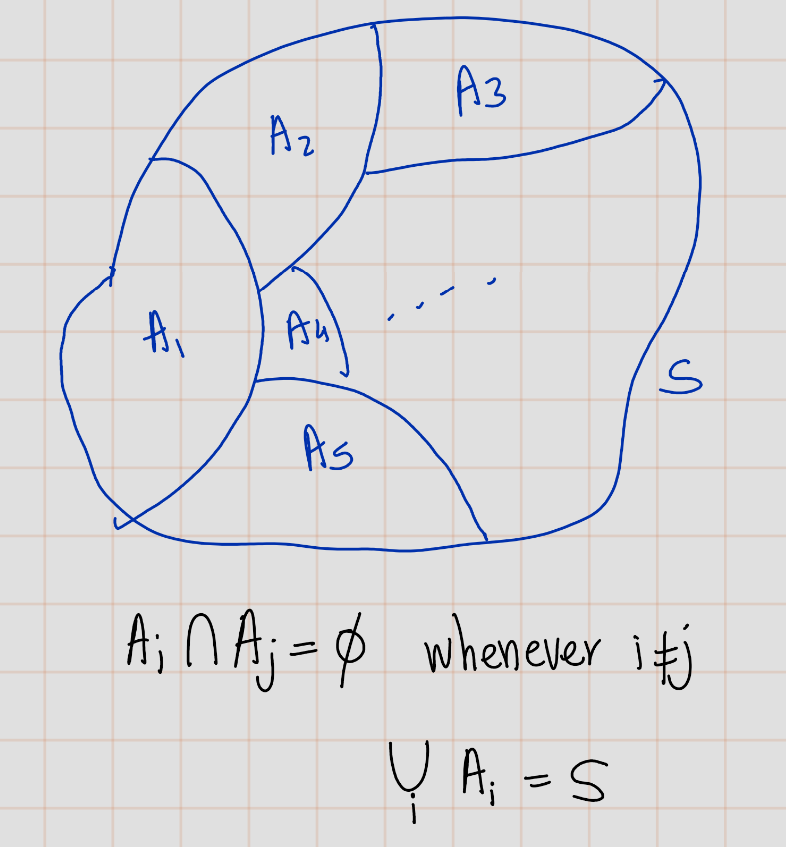
\includegraphics{figures/ch_2/fig32.png}

\begin{example}
\protect\hypertarget{exm:unnamed-chunk-21}{}\label{exm:unnamed-chunk-21}The two sets \emph{Even} and \emph{Odd} partition the set of integers.
\end{example}

\begin{example}
\protect\hypertarget{exm:unnamed-chunk-22}{}\label{exm:unnamed-chunk-22}With the usual notation, the sets
\[\{1\}, \{y, xy, x^2y\}, \{x, x^2\}\]
form a partition of the symmetric group \(S_3\).
\end{example}

\begin{definition}
\protect\hypertarget{def:unnamed-chunk-23}{}\label{def:unnamed-chunk-23}

An equivalence relation on a set \(S\) is a relation that holds between certain pairs of elements.

\begin{itemize}
\tightlist
\item
  Reflexive: For all \(a\), \(a \sim a\).
\item
  Symmetric: If \(a \sim b\) , then \(b \sim a\).
\item
  Transitive: If \(a \sim b\) and \(b \sim c\) , then \(a \sim c\).
\end{itemize}

\end{definition}

\begin{example}
\protect\hypertarget{exm:unnamed-chunk-24}{}\label{exm:unnamed-chunk-24}Two triangles are said to be congruent if their sides have the same length and angles have same measure.\\
Congruence of triangles is an example of an equivalence relation on the set of triangles in the plane. If \(A , B,\) and \(C\) are triangles, and if \(A\) is congruent to \(B\) and \(B\) is congruent to \(C\), then \(A\) is congruent to \(C\). It is very easy to check three equivalnace propoties. I am not going to do this.
\end{example}

\begin{example}
\protect\hypertarget{exm:unnamed-chunk-25}{}\label{exm:unnamed-chunk-25}

Conjugacy is an equivalence relation on a group.
Let \(G\) be garoup Two group elements are conjugate, \(a\sim b\), if \(b = gag^{- 1}\) for some \(g\in G\).

\begin{itemize}
\tightlist
\item
  \emph{Reflexive}: Observe that \(a=aaa^{-1}\) then, \(a\sim a\).
\item
  \emph{Symmetric}: Suppose that \(a\sim b\), then \(b=gag^{-1}\). Thus,
  \(a=g^{-1}bg\). Hence, \(b \sim a\).
\item
  \emph{Transitive}: Suppose that \(a\sim b\) and \(b \sim c\). This means that \(b = g_1ag_1^{-1}\) and \(c = g_2bg_2^{-1}\) for some group elements \(g_1\) and \(g_2\).
  Then \(c = g_2(g_1ag_1^{-1})g_2^{-1} = (g_2 g_1)a (g_2 g_1),\) ~so \(a \sim c\)
\end{itemize}

\end{example}

\begin{proposition}
\protect\hypertarget{prp:unnamed-chunk-26}{}\label{prp:unnamed-chunk-26}An equivalence relation on a set S determines a partition of S, and conversely.
\end{proposition}

\begin{proof}
\leavevmode

\begin{itemize}
\tightlist
\item
  (\(\Longrightarrow\)): Given a partition of \(S\), the corresponding equivalence relation is defined by the rule
  that \(a \sim b\) if \(a\) and \(b\) lie in the same subset of the partition. The axioms for an equivalence relation are obviously satisfied.
\item
  (\(\Longrightarrow\)): Given an equivalence relation (\(\sim\)), one defines a partition this way:\\
  The subset that contains \(a\) is the set of all elements \(b\) such that \(a \sim b\). This subset is called the \textbf{equivalence class} of a. We'll denote it by \(C_a\) here
  \[C_a = \{b \in S | a\sim b\}\]
  The next lemma completes the proof of the proposition
\end{itemize}

\end{proof}

\begin{lemma}
\protect\hypertarget{lem:unnamed-chunk-28}{}\label{lem:unnamed-chunk-28}Given an equivalence relation on a set \(S\), the subsets of \(S\) that are equivalence classes partition \(S\).
\end{lemma}

\begin{proof}

This is an important point, so we will check it carefully. We must remember that the notation \(C_a\) stands for a subset defined in a certain way. The partition consists of the subsets, and several notations may describe the same subset.

\begin{itemize}
\item
  \emph{Non-emptyness}: The reflexive axiom tells us that \(a\) is in its equivalence class. Therefore, the class \(C_a\) is nonempty.
\item
  \emph{Union is whole set}: Since \(a\) can be any element, the union of the equivalence classes is the whole set \(S\).
\item
  \emph{Disjoint property}: To show this, we prove follwoing calim:

  \begin{itemize}
  \tightlist
  \item
    \textbf{Claim}: \(\text{If } C_a \text{ and } C_b \text{ have an element in common, then } C_a = C_b\).\\
    Since we can interchange the roles of \(a\) and \(b\), it will suffice to show that if \(C_a\) and \(C_b\) have an element, say \(d\), in common, then \(C_b \subseteq C_a\).\\
    Sippose that \(x\) is in \(C_b\), then \(b \sim x\). Since \(d\) is in both sets, \(a \sim d\) and \(b \sim d\), and the symmetry property tells us that \(d \sim b\). So we have \(a \sim d\), \(d \sim b\), and \(b \sim x\). Two applications of transitivity show that \(a \sim x\), and therefore, \(x\) is in \(C_a\).
  \end{itemize}
\end{itemize}

\end{proof}

\begin{example}
\protect\hypertarget{exm:272}{}\label{exm:272}The relation on a group defined by \(a ~ b\) if \(a\) and \(b\) are elements of the same order is an equivalence relation. ( Trivial.)

The corresponding partition for the symmetric group S3 are
\[\{1\}, \{y, xy, x^2y\}, \{x, x^2\}.\]
\end{example}

If a partition of a set \(S\) is given, we may construct a new set \(\overline{S}\) whose elements are the subsets. We imagine putting the subsets into separate piles, and we regard the piles as the elements of our new set \(\overline{S}\). It seems advisable to have a notation to distinguish a subset from the element of the set \(S\) (the pile) that it represents. If \(U\) is a subset, we will denote by \([U]\) the corresponding element of \(S\).

\begin{example}
\protect\hypertarget{exm:unnamed-chunk-30}{}\label{exm:unnamed-chunk-30}If \(S\) is the set of integers and if \(\text{Even}\) and \(\text{Odd}\) denote the subsets of even and odd integers, respectively, then \(\overline{S}\) contains the two elements \([\text{Even}]\) and \([\text{Odd}]\).
\end{example}

We will use this notation more generally. When we want to regard a subset \(U\) of \(S\) as an element of a set of subsets of \(S\), we denote it by \([U]\).

When an equivalence relation on \(S\) is given, the equivalence classes form a partition, and we obtain a new set \(\overline{S}\) whose elements are the equivalence classes \([C_a]\). We can think of the elements of this new set in another way, as the set obtained by changing what we mean by equality among elements. If \(a\) and \(b\) are in \(S\), we interpret \(a \sim b\) to mean that \(a\) and \(b\) become equal in \(\overline{S}\), because \(C_a = C_b\). With this way of looking at it, the difference between the two sets \(S\) and \(\overline{S}\) is that in \(\overline{S}\) more elements have been declared ``equal,'' i.e., equivalent. It seems to me that we often treat congruent triangles this way in school.

For any equivalence relation, there is a natural surjective map
\begin{equation}
 \quad \pi : S \to \overline{S}
\end{equation}
that maps an element \(a\) of \(S\) to its equivalence class: \(\pi(a) = [C_a]\). When we want to regard \(\overline{S}\) as the set obtained from \(S\) by changing the notion of equality, it will be convenient to denote the element \([C_a]\) of \(\overline{S}\) by the symbol \(a\). Then the map \(\pi\) becomes
\begin{equation}
\pi(a) = \overline{a}
\end{equation}

We can work in \(\overline{S}\) with the symbols used for elements of \(S\), but with bars over them to remind us of the new rule:
\begin{equation}
\text{If } a \text{ and } b \text{ are in } S, \text{ then } \overline{a} = \overline{b} \text{ means } a \sim b.
\end{equation}

A disadvantage of this bar notation is that many symbols represent the same element of \(S\). Sometimes this disadvantage can be overcome by choosing a particular element, a representative element, in each equivalence class. For example, the even and the odd integers are often represented by \(\overline{0}\) and \(\overline{1}\):
\begin{equation}
\{[\text{Even}], [\text{Odd}]\} = \{ \overline{0}, \overline{1}\}.
\end{equation}

Though the pile picture may be easier to grasp at first, the second way of viewing \(S\) is often better because the bar notation is easier to manipulate algebraically.

\hypertarget{the-equivalence-relation-defined-by-a-map}{%
\subsection{The Equivalence Relation Defined by a Map}\label{the-equivalence-relation-defined-by-a-map}}

Any map of sets \(f : S \to T\) gives us an equivalence relation on its domain \(S\). It is defined by the rule: \(a \sim b\) if \(f(a) = f(b)\).

\begin{definition}[Inverse Image  and Fibers]
\protect\hypertarget{def:unnamed-chunk-31}{}\label{def:unnamed-chunk-31}The inverse image of an element \(t\) of \(T\) is the subset of \(S\) consisting of all elements \(s\) such that \(f(s) = t\). It is denoted symbolically as
\begin{equation}
f^{-1}(t) = \{s \in S \mid f(s) = t\}.
\end{equation}

The inverse images are also called the fibres of the map \(f\) , and the fibres that are not empty are the equivalence classes for the relation defined above.
\end{definition}

\begin{remark}
This is symbolic notation. Please remember that \textbf{unless \(f\) is bijective, \(f^{-1}\) will not be a map}.
\end{remark}

Here the set S of equivalence classes has another incarnation, as the image of the map.
The elements of the image correspond bijectively to the nonempty fibres, which are the
equivalence classes

\begin{example}
\protect\hypertarget{exm:unnamed-chunk-33}{}\label{exm:unnamed-chunk-33}Let's consider the absolute value map from the complex numbers \(\mathbb{C}^\times\) to the positive real numbers \(\mathbb{R}^+\):

\[ f: \mathbb{C}^\times \to \mathbb{R}^+, \quad f(z) = |z| \]

The fiber of an element \(t\) in \(\mathbb{R}^+\) is the subset of \(\mathbb{C}^\times\) consisting of all complex numbers \(z\) such that \(f(z) = |z| = t\). Symbolically, we denote the fiber as:

\[ f^{-1}(t) = \{ z \in \mathbb{C}^\times : |z| = t \} \]

This fiber represents all complex numbers with the same absolute value \(t\). Thus, fibers are circles in Complex plane.

Note that the absolute value map is surjective, so each positive real number \(t\) corresponds to a unique fiber in \(\mathbb{C}^\times\).
\end{example}

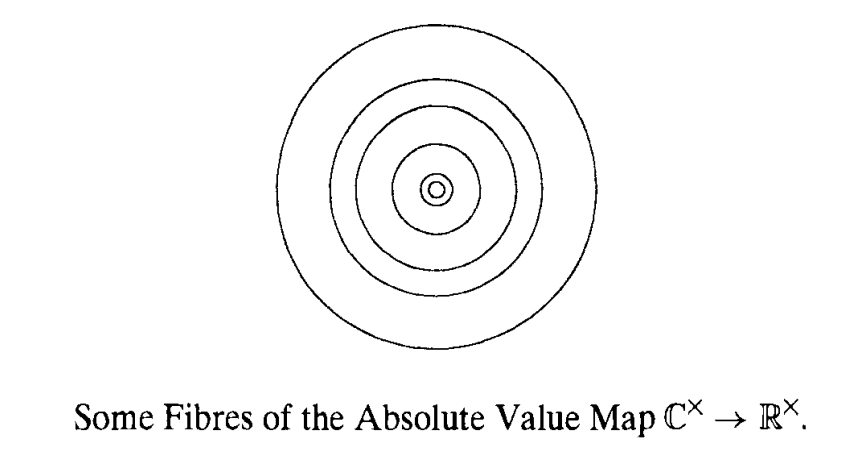
\includegraphics{figures/ch_2/fig33.png}

\begin{example}
\protect\hypertarget{exm:unnamed-chunk-34}{}\label{exm:unnamed-chunk-34}If \(G\) is a finite group, we can define a map \(f : G \to \mathbb{N}\) to the set \(\{1, 2, 3, \ldots\}\) of natural numbers, letting \(f(a)\) be the order of the element \(a\) in \(G\). The fibers of this map are the sets of elements with the same order (see example \ref{exm:272}).
\end{example}

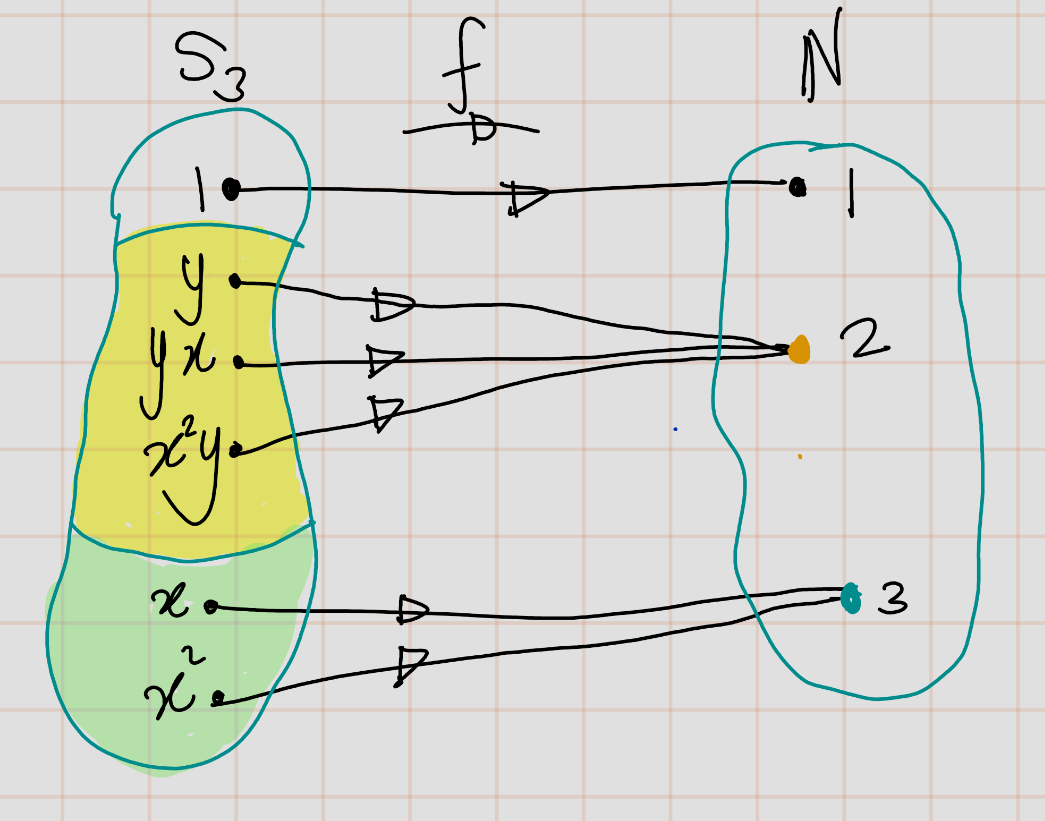
\includegraphics{figures/ch_2/fig34.png}

\begin{definition}[congruence]
\protect\hypertarget{def:unnamed-chunk-35}{}\label{def:unnamed-chunk-35}Let \(G,G'\) be a groups and \(\phi: G \rightarrow G'\) be a group group homomorphism. The equivalence relation on \(G\) defined by \(\phi\) is usually denoted by \(\equiv\), rather than by \(\sim\), and is referred to as congruence.
\[a \equiv b \text{ if }\phi(a) = \phi(b)\]
\end{definition}

We have seen that elements \(a\) and \(b\) of \(G\) are congruent, i.e., \(\phi(a) = \phi(b)\), if and only if \(b\) is
in the coset \(a K\) of the kernel \(K\) (See proposition \ref{prp:258})

\begin{proposition}
\protect\hypertarget{prp:unnamed-chunk-36}{}\label{prp:unnamed-chunk-36}Let \(K\) be the kernel of a homomorphism \(\varphi: G \to G'\). The fibre of that contains an element \(a\) of \(G\) is the coset \(a K\) of \(K\). These cosets partition the group \(G\), and they correspond to elements of the image of \(\varphi\).
\end{proposition}

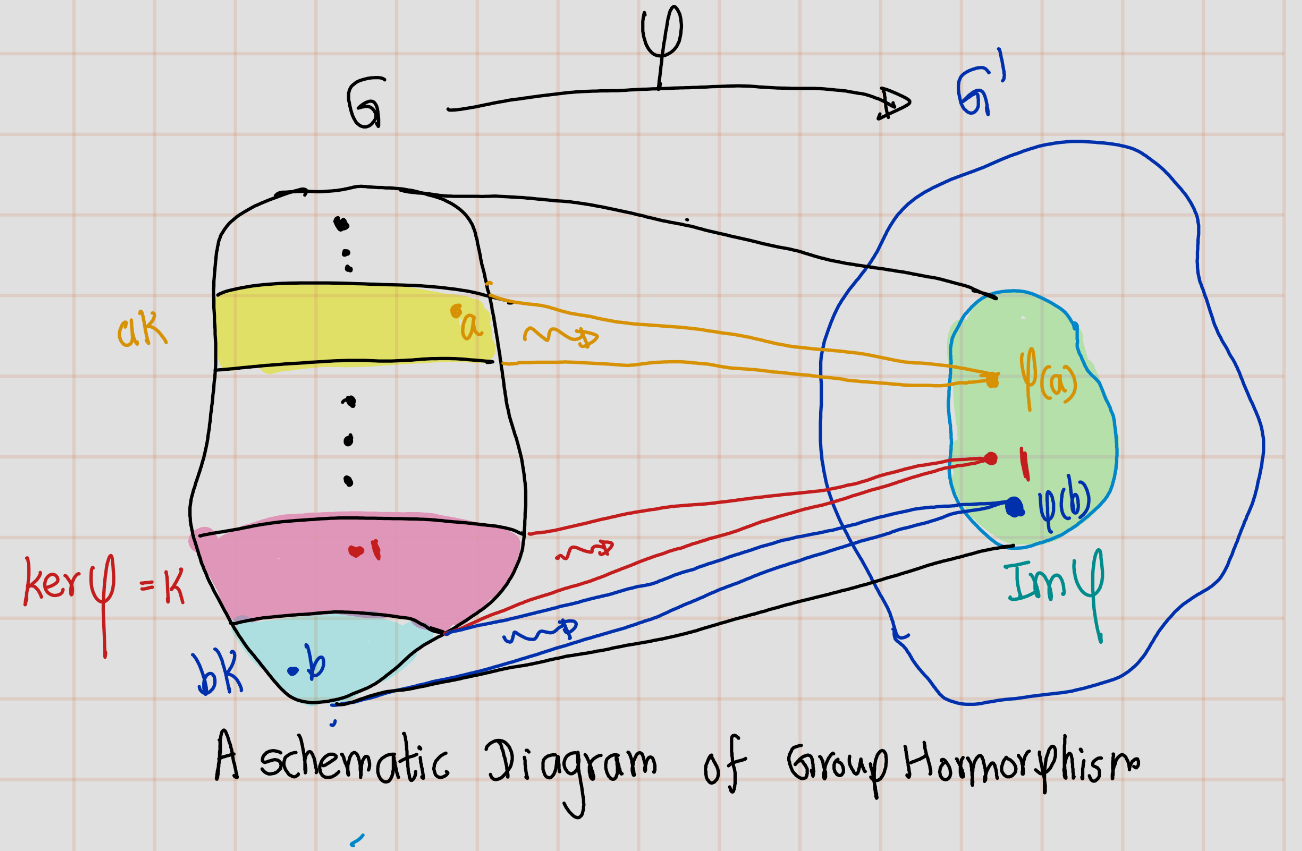
\includegraphics{figures/ch_2/fig35.png}

\begin{proof}
The fibre of \(\varphi\) over an element \(g' \in G'\) is the set of all elements \(a \in G\) such that \(\varphi(a) = g'\). Let's denote this fibre as
\[F_{g'} = \{a \in G : \varphi(a) = g'\}\].

Now, let's take an arbitrary element \(a \in G\) and consider the left coset \(aK = \{ak : k \in K\}\).

We know that \(K\) is the kernel of \(\varphi\), so for any \(k \in K\), we have \(\varphi(k) = 1_{G'}\) where \(1_{G'}\) is the identity element in \(G'\).

\begin{itemize}
\tightlist
\item
  Claim 1: \(aK=F_{\varphi(a)}\).

  \begin{itemize}
  \item
    sub claim 1.1: \(aK \subseteq F_{\varphi(a)}\).\\
    For any \(ak \in aK\), we have \(\varphi(ak) = \varphi(a)\varphi(k) = \varphi(a)1_{G'} = \varphi(a)\).This shows that every element in the coset \(aK\) is mapped to the same element under \(\varphi\) as \(a\) itself. Therefore, the coset \(aK\) is a subset of the fibre \(F_{\varphi(a)}\).
  \item
    sub claim 1.2 : \(F_{\varphi(a)}\subseteq aK\).\\
    If \(a' \in F_{\varphi(a)}\), then \(\varphi(a') = \varphi(a)\), which implies that \(\varphi((a')^{-1}a) = 1_{G'}\).
    This means that \((a')^{-1}a \in K\), or equivalently, \(a' \in aK\). (by proposition \ref{prp:258})Therefore, the fibre \(F_{\varphi(a)}\) is a subset of the coset \(aK\).
  \end{itemize}
\end{itemize}

Since \(aK\) is a subset of \(F_{\varphi(a)}\) and \(F_{\varphi(a)}\) is a subset of \(aK\), we conclude that \(aK = F_{\varphi(a)}\). So, the fibre of \(\varphi\) that contains an element \(a\) of \(G\) is indeed the coset \(aK\) of \(K\).

\begin{itemize}
\tightlist
\item
  Claim 2: The cosets of a subgroup \(K\) partition the group \(G\).
\end{itemize}

A partition of a set is a collection of non-empty subsets such that every element in the set is in exactly one of these subsets.

To show that the cosets of \(K\) partition \(G\), we need to show two things:

\begin{itemize}
\item
  sub claim 2.1: Every element of \(G\) is in at least one coset of \(K\).\\
  Given any \(g \in G\), \(g\) is in the coset \(gK\). So, every element of \(G\) is in at least one coset of \(K\).
\item
  sub claim 2.2: No element of \(G\) is in more than one coset of \(K\)\\
  Suppose \(gK\) and \(hK\) are two cosets of \(K\) and there is some element \(x \in G\) that is in both \(gK\) and \(hK\). This means that there exist \(k_1, k_2 \in K\) such that \(x = gk_1 = hk_2\) (by proposition \ref{prp:258}. Then \(g = hk_2k_1^{-1}\). Thus, \(g\in gK\), which implies that \(gK = hK\).
  So, no element of \(G\) is in more than one coset of \(K\).
\end{itemize}

Therefore, the cosets of \(K\) partition the group \(G\).
\end{proof}

\hypertarget{cosets}{%
\section{Cosets}\label{cosets}}

\hypertarget{modular-arithmetic}{%
\section{Modular Arithmetic}\label{modular-arithmetic}}

\hypertarget{the-correspondence-theorem}{%
\section{The Correspondence Theorem}\label{the-correspondence-theorem}}

\begin{definition}
\protect\hypertarget{def:unnamed-chunk-38}{}\label{def:unnamed-chunk-38}Let \(\phi: G \rightarrow G^\prime\) be a group homomorphism, and let \(H\) be a subgroup of \(G\). We may restrict \(\phi\) to \(H\), obtaining a homomorphism
\[\phi|_H: H \rightarrow G^\prime\]
\end{definition}

In other words, we take the same map but restrict its domain.

\textbf{Notation}: We use this notation for clarity \([\phi|_H](h)\).

Further, we can see that follwoing observatons.

\begin{itemize}
\tightlist
\item
  By definition, \(\forall h\in H,\phi|_H(h) = \phi(h)\)
\item
  The restriction \(\phi|_H\) is a homomorphism (Since \(\phi\) is homomorphism).
\item
  The kernel of \(\phi|_H\) is the intersection of the kernel of \(\phi\) with \(H\):
  \[ker(\phi|_H) = (ker\phi) \cap H\]
  There is no need to prove this. This is trivial by definition of kernel.
\item
  Image of \(\phi|_H\) is the same as the image \(\phi(H)\) of \(H\) under the map \(\phi\).
  \[Im(\phi_H)=\phi(H)\]
\item
  If \(|H|\) and \(|G'|\) have no common factor, \(\phi(H) = \{1\}\), so \(H\) is contained in the kernel.
  (Since, by Artin's book corollary 2.8.13,
\end{itemize}

\begin{eqnarray}
|Im(\phi_H)|&\biggr |&|H|\\
|Im(\phi_H)|&\biggr |& |G'|
\end{eqnarray}, Thus, if \(|H|\) and \(|G'|\) have no common factors,\(|Im(\phi_H)|=|\phi(H)| =1.\) So, \(Im(\phi_H)=\phi(H)= \{1\}\)

Now let's see an example.

\begin{example}
\protect\hypertarget{exm:unnamed-chunk-39}{}\label{exm:unnamed-chunk-39}Define sign homorphism \(\sigma: S_n \to \{\pm 1\}\) by \(\sigma(x)=1\) if \(x\) is even, and \(\sigma (x)=-1\) if \(x\) is odd. Then the image of the sign homomorphism is,
\[Im(\sigma)=\{\pm 1\}\]
it has order \(2\).

Let \(H=\{x \in S_n : \text{if $x$ has odd order}\}\). Then \(H\) is a subgroup. So,, \(H \subset \ker(\sigma)\) (We can easily verify this.)

Furthur, The sub group of \(S_n\) with even permutations is called \emph{Alternating group} (\(A_n\)).
\end{example}

\hypertarget{problem}{%
\subsection{PROBLEM}\label{problem}}

\begin{proposition}
\protect\hypertarget{prp:2104}{}\label{prp:2104}

Let \(\phi:G \to G^{\prime}\) be a homomorphism with kernel \(K\), and let \(H^\prime\leq G^\prime\). Denote the inverse image \(\phi^{-1}(H^\prime)\) by \(H\). i.e.:

\[H=\phi^{-1}(H^\prime)=\{x\in G: \phi(x)\in H^\prime\}\]
Then,

\begin{itemize}
\tightlist
\item
  \(\phi^{-1}(H^\prime)\) is a subgroup of \(G\) that contains \(K\).
\item
  If \(H\) is a normal subgroup of \(G^\prime\), then \(\phi^{-1}(H^\prime)\) is also a normal subgroup of \(G\).
\item
  If \(\phi\) is surjective and \(H\) is a normal subgroup of \(G\), then \(\phi^{-1}(H^\prime)\) is a normal subgroup of \(G^\prime\).
\end{itemize}

\end{proposition}

\begin{remark}
\(\phi^{-1}\) is not a map.
\end{remark}

\begin{proof}
\leavevmode

\begin{itemize}
\tightlist
\item
  \textbf{Claim 1}: \(K\subseteq \phi^{-1}(H^\prime)=H\)\\
  Let \(x\in K\). Then \(\phi(x)=1_{G^\prime}\). Since \(1_{G^\prime}\in H^\prime\). Thus, \(x\in \phi^{-1}(H^\prime)=H\). Therfore, \(K\subseteq \phi^{-1}(H^\prime)=H\)
\item
  \textbf{Claim 2}: \(\phi^{-1}(H^\prime)\) is a subgroup of \(G\)\\

  \begin{itemize}
  \tightlist
  \item
    \emph{Closure} :Suppose \(x,y\in H= \phi^{-1}(H^\prime)\). Then \(\phi(x),\phi(y)\in \phi(H^\prime)\). Since \(\phi\) is hormophism \(\phi(x)\phi(y)=\phi(xy)\). Since \(H^\prime\leq G^\prime\), then \(\phi(xy)=\phi(x)\phi(y)\in H^\prime\). Thus, \(xy\in \phi^{-1}(H^\prime)=H\)
  \item
    \emph{Identity} : Since \(\phi(1_G)=1_{G^\prime}\), \(1_G\in \phi^{-1}(H^\prime)=H\)
  \item
    \emph{Inverse} : Let \(x\in \phi^{-1}(H^\prime)=H\). Then \(\phi(x)\in H^\prime\) and since \(H^\prime \leq G^\prime\),then \((\phi(x))^{-1}\in H^\prime\). Since \(\phi\) is a homomorphism, \((\phi(x))^{-1}=\phi(x^{-1})\), Thus \((\phi(x))^{-1}=\phi(x^{-1})\in H^\prime\). Hence, \(x^{-1}\in \phi^{-1}(H^\prime)\).
  \end{itemize}
\item
  \textbf{Claim 3}: If \(H^\prime\) is a normal subgroup of \(G^\prime\), then \(\phi^{-1}(H^\prime)\) is also a normal subgroup of \(G\).\\
  Now suppose that \(H^\prime\) is a normal subgroup of \(G^\prime\). Let \(x\in H\) and \(g\in G\). Then, since \(\phi\) is hormorphism,
  \[\phi(-1)=\phi(g)\phi(x)\phi(g^{-1})=\phi(g)\phi(x)(\phi(g))^{-1}\]
  So, \(\phi(gxg^{-1})\) is conjugate of \(\phi(x)\). Since \(x\in H=\phi^{-1}(H^\prime)\),the \(\phi(x)\in H^\prime\). Thus, \(\phi(gxg^{-1})=\phi(g)\phi(x)(\phi(g))^{-1}\in H^\prime\). Hence,
  \(gxg^{-1}\in \phi^{-1}(H^\prime)=H\).
\item
  \textbf{Claim 4}: If \(\phi\) is surjective and \(H\) is a normal subgroup of \(G\), then \(\phi^{-1}(H^\prime)\) is a normal subgroup of \(G^\prime\).\\
  Suppose that \(\phi\) is surjective and \(H\) is a normal subgroup of \(G\). Let \(a\in H^\prime\) and \(b\in G^\prime\). Since \(\phi\) is surjcetive, There are elements \(x\in H\) and \(y\in G\) such that \(\phi(x) = a\) and \(\phi(y) = b\). Since \(H\) is normal \(yxy^{- 1}\in H\), thus \(\phi(yxy^{-1})=bab^{-1}\in H^\prime\).
\end{itemize}

\end{proof}

\begin{example}
\protect\hypertarget{exm:unnamed-chunk-42}{}\label{exm:unnamed-chunk-42}let denote the determinant homomorphism \[det:GL_n(\mathbb{R})\to \mathbb{R}^\times\]. Note that \(\mathbb{R}^+\unlhd \mathbb{R}^\times\). (It is very clear that \$The set of positive real numbers is a subgroup of \(\mathbb{R}^\times\), and since \(\mathbb{R}^\times\) is abliean, \(\mathbb{R}^+\) is normal.) Now consider the inverse image of \(\mathbb{R}^+\),
\[det^{-1}(\mathbb{R}^+)=\{A\in GL_n(\mathbb{R}):det(A)\in \mathbb{R}^+\}=SL_n(\mathbb{R})\]. By above proposition we can ge that \(SL_n(\mathbb{R})\) is normal subgroup. (Because \(\mathbb{R}^+\unlhd \mathbb{R}^\times\) and \(det\) is surjective map.)
\end{example}

\begin{theorem}[Correspondence Theorem]
\protect\hypertarget{thm:CorrespondenceTheorem}{}\label{thm:CorrespondenceTheorem}

Let \(\phi: G \to G^\prime\) be a surjective group homomorphism with kernel \(K\). There is a bijective correspondence between subgroups of \(G^\prime\) and subgroups of \(G\) that contain \(K\):
\[\{\text{subgroups of $G$ that contain $K$}\}\longleftrightarrow \{\text{subgroups of $G^\prime$}\}\]
This corresponde nce is defined as follows:
\[\begin{aligned}
\text{a subgroup $H$ of $G$ that contains K} &\rightsquigarrow \text{ its image} (\phi(H) \in G^\prime,\\
\text{a subgroup $H^\prime$ of $G^\prime$} &\rightsquigarrow \text{ its inverse image $\phi^{-1}(H^\prime)$ in $G$}.
\end{aligned}\]

\begin{itemize}
\tightlist
\item
  If \(H\) and \(H^\prime\) are corresponding subgroups, then \(H\) is normal in \(G\) if and only if is normal in \(G^\prime\).
\item
  If If \(H\) and \(H^\prime\) are corresponding subgroups, then
  \[|H|= |H^\prime||K |\]
\end{itemize}

\end{theorem}

\begin{proof}
Let \(H\) be subgroup of \(G\) that contain \(K\). Let \(H^\prime\) be a subgroup of \(G^\prime\). Now we need to check folllwings,

\begin{itemize}
\item
  \(\phi(H)\) is a subgroup of \(G^\prime\).
\item
  \(\phi^{-1}(H^\prime)\) is a subgroup of \(G\), and it contains \(K\).
\item
  \(H^\prime\) is a normal subgroup of \(G^\prime\) if and only if \(\phi^{-1}(H^\prime)\) is a normal subgroup of \(G\).
\item
  (\emph{bijectivity of the correspondence}) \(\phi(\phi^{-1}(H^\prime)) =H^\prime\) and \(\phi^{-1}(\phi(H))=H\)
\item
  \(|(\phi^{-1} (H^\prime)| = |H^\prime||K|\).
\item
  \textbf{Claim 1}: \(\phi(H)\) is a subgroup of \(G^\prime\).\\

  \begin{itemize}
  \tightlist
  \item
    \emph{Closure}: Let \$\(x,y\in phi(H)\). Then there is \(a,b\in H\) such that \(\phi(a)=x\) and \(\phi(b)=y\). Since \(\phi\) is hormorphism, \(xy=\phi(a)\phi(b)=\phi(ab)\). Sine \(H\leq G\), \(ab\in H,~ xy=\phi(ab)\in \phi(H)\).
  \item
    \emph{Identity} : Since \(1_G\in H\), \(\phi(1_G)=1_{G^\prime}\in \phi(H)\)
  \item
    \emph{Inverse} : Let \(x\in \phi(H)\). Then there exist \(a\in H\) such that \(\phi(a)=x\). Since \(H\leq G\), \(a^{-1}\) exists in \(H\). \(\phi(a^{-1})=\phi(a)^{-1}=x^{-1}\in \phi(G)\).
  \end{itemize}
\item
  \textbf{Claim 2}: \(\phi^{-1}(H^\prime)\) is a subgroup of \(G\), and it contains \(K\).\\
  This is true from proportion \ref{prp:2104}
\item
  \textbf{Claim 3}: \(H^\prime\) is a normal subgroup of \(G^\prime\) if and only if \(\phi^{-1}(H^\prime)\) is a normal subgroup of \(G\).\\
  Alreday this prooved in proportion \ref{prp:2104}
\item
  \textbf{Claim 4.1}: \(\phi(\phi^{-1}(H^\prime))=H^\prime\)

  \begin{itemize}
  \item
    \(\phi(\phi^{-1}(H^\prime))\subset H^\prime\)\\
    Lett \(x\in \phi(\phi^{-1}(H^\prime))\).
    Then there exist \(y\in\phi^{-1}(H^\prime)\) such that \(\phi(y)=x\). Then by definiton of the pre image \(x=\phi(y)\in H^\prime\).
  \item
    \(\phi(\phi^{-1}(H^\prime))\supset H^\prime\)\\
    Let \(a\in H^\prime\). Since \(\phi\) is surjective, there exists \(b\in G\) such that \(\phi(b)=a\in H^\prime\). Thus \(b\in \phi^{-1}(H^\prime)\). Hence \(a=\phi(b)=\phi(\phi^{-1}(H^\prime))\).
  \end{itemize}
\end{itemize}

Therefore, \(\phi(\phi^{-1}(H^\prime))=H^\prime\).

\begin{itemize}
\tightlist
\item
  \textbf{Claim 4.2}: \(\phi^{-1}(\phi(H))=H\)

  \begin{itemize}
  \tightlist
  \item
    \(\phi^{-1}(\phi(H))\supset H\)\\
    Let \(x\in H\). Then \(\phi(x) \in \phi(H)\). So, \(x\in \phi^{-1}(\phi(H))\).
  \item
    \(\phi^{-1}(\phi(H))subset H\)\\
    Let \(y\in \phi^{-1}(\phi(H))\). By definition of inverse image, \(\phi(y)\in \phi(H)\). Then there exist \(z\in H\) such that \(\phi(y)=\phi(z)\). Then \(z^{-1}y\) is in the kernal \(K\).(by Artins book proposition 2.5.8). Since \(K \subset H\), \(z^{-1}y\in H\). So, \(a\in H\) and \(a^{-1}z\in H\). Thus, \(a(a^{-1}x)=x\in H\). Hence \(\phi^{-1}(\phi(H))\subset H\)
  \end{itemize}
\end{itemize}

Therefore, \(\phi^{-1}(\phi(H))=H\)
- \textbf{Claim 5} : \(|(\phi^{-1} (H^\prime)| = |H^\prime||K|\).\\

\end{proof}

\hypertarget{problem-1}{%
\subsection{Problem}\label{problem-1}}

\begin{example}
\protect\hypertarget{exm:unnamed-chunk-44}{}\label{exm:unnamed-chunk-44}Recall

\[\begin{aligned}
S_4 &= \left\{ id, (1 2), (1 3), (1 4), (2 3), (2 4), (3 4), (1 2 3), (1 2 4), (1 3 2), (1 3 4), (1 4 2), (1 4 3), (2 3 4), (1 2 3 4) \right\}\\
S_3 &= \left\{ id, (1 2), (1 3), (2 3), (1 2 3), (1 3 2) \right\}
\end{aligned}\]

There are 6 such subgroups of \(S_3\),\[ <(1 2)>, <(1 3)>, <(2 3)>, <(1 2 3)>= <(1 3 2)>,S_3\].
There is one proper subgroup of order 3. That is \(<(123)>\). There are 3 subgroups of order 2. They are \(<(1 2)>, <(1 3)>, <(2 3)>\)

The Correspondence Theorem tells us that there are four proper
subgroups of \(S_4\) that contain \(K\).
\end{example}

\hypertarget{problem-2}{%
\subsection{Problem}\label{problem-2}}

\hypertarget{product-groups}{%
\section{Product Groups}\label{product-groups}}

Let \(G,G'\) be two groups. The product set \(G \times G'\), the set of pairs of elements \((a, a')\) with
a in G and a' in G', can be made into a group by component-wise multiplication,

multiplication of pairs is defined by the rule,

\[(a,a')\cdot(b,b')=(ab,a'b')\quad \text{for } a,b\in  G \text{ and for } a',b'\in G\]
Let's prove that \(G\times G'\) is a group.

\begin{proof}

Let \(G,G'\) be two groups and let \(a,b,c\in G\) and \(a',b',c'\in G'\)

\begin{itemize}
\tightlist
\item
  \emph{Closure} : \((a,a')\cdot (b,b')=(ab,a'b')\). So, since \(a,b\in G\) and \(a',b'\in G'\) and \(G\) and \(G'\) be a group, then \(ab\in G\) and \(a'b'\in G\). Thus, \((a,a')\cdot(b,b')=(ab,a'b')\in G \times G'\).
\item
  \emph{Asscitivity}: We can obtain following using asscivity property of group \(G\) and \(G'\).
  \[((a,a')\cdot(b,b'))\cdot(c,c')=(ab,a'b')\cdot(c,c')
  =(abc,a'b'c')=
  (a,a')\cdot(bc,b'c')=(a,a')\cdot((b,b')\cdot(c,c'))\]
\item
  \emph{identity}: (1\_G,1\_\{G'\}) is the idenitity\\
  \[(1_G,1_{G'})\cdot(b,b')=(1_Gb,1_{G'}b')=(b,b')
  =(b1_G,b'1_{G'})=(b,b')\cdot(1_G,1_{G'})\]
\item
  \emph{Inverse} : The inverse of \((a,a')\) is \((a^{-1},(a')^{-1})\)\\
  \[(a,a')\cdot(a^{-1},(a')^{-1})=(aa^{-1},a'(a')^{-1})=(1_G,1_{G'})=(a^{-1}a,(a')^{-1}a')=(a^{-1},(a')^{-1})\cdot(a,a')\]
\end{itemize}

\end{proof}

So, The group obtained in this way is called the product of \(G\) and \(G'\).

It is related to the two factors \(G\) and \(G'\) in a simple way that we can sum up in terms of some homomorphisms.
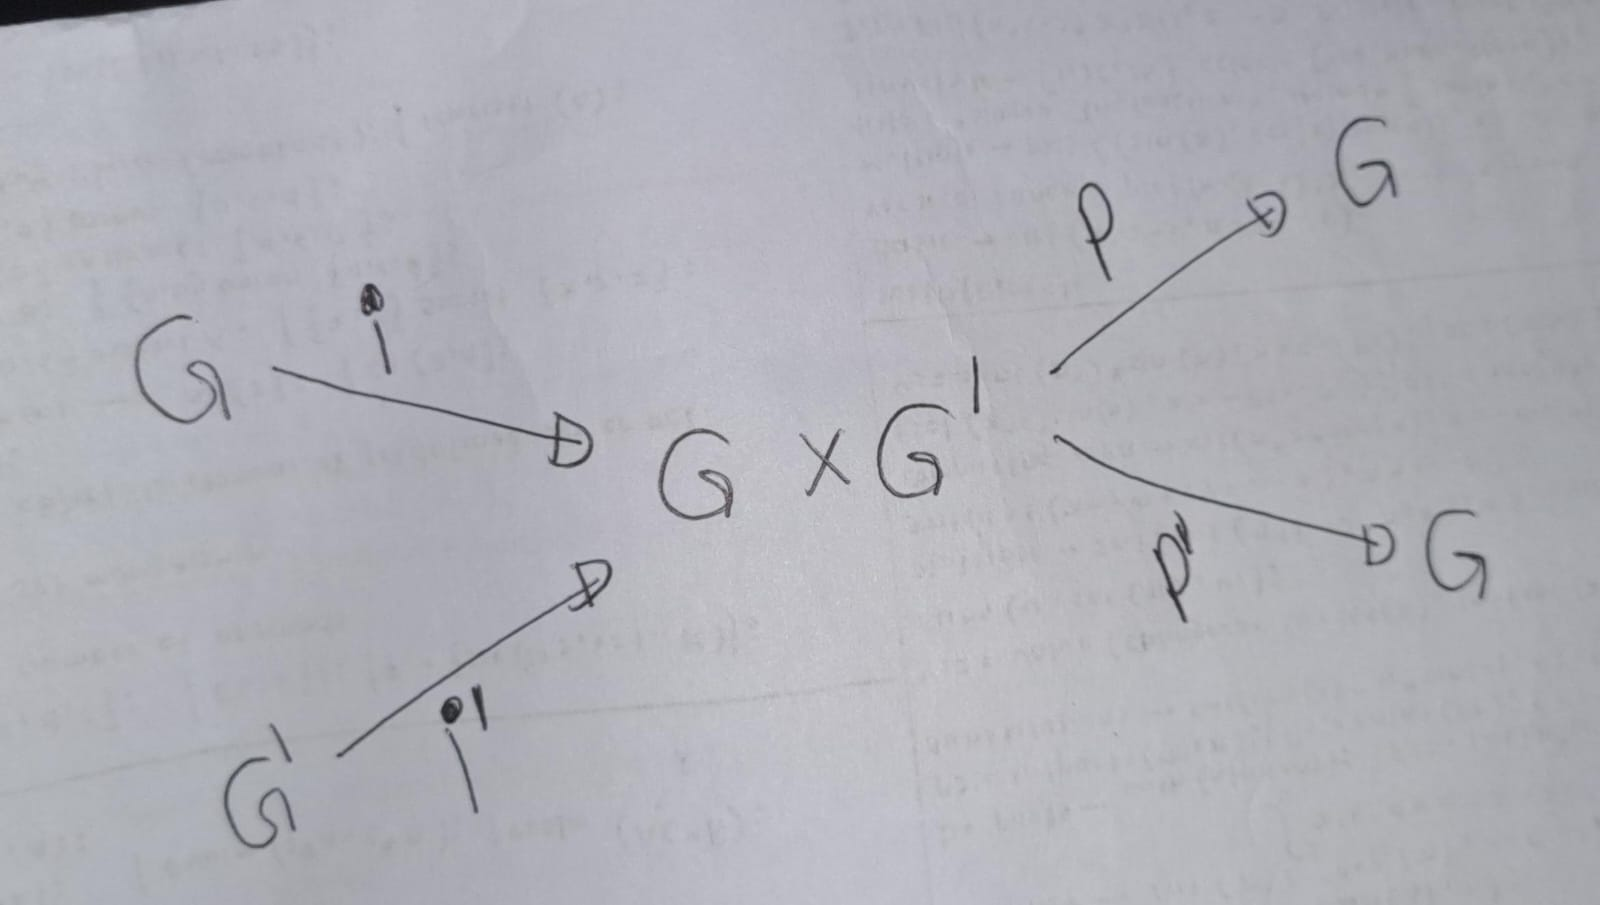
\includegraphics{figures/ch_2/fig01.jpg}
The homomorphisms are defined as follows,
\begin{eqnarray}
i:G &\rightarrow& G \times G' \\
x &\mapsto& (x,1)\\\\
i':G' &\rightarrow& G \times G' \\
x &\mapsto& (x',1)\\\\
p:G \times G' &\rightarrow& G' \\
(x,x') &\mapsto& x\\\\
p':G' \times G' &\rightarrow& G' \\
(x,x') &\mapsto& x'\\\\
\end{eqnarray}

Observe that \(i\) and \(i'\) are injective and \[Im(i)=G\times 1_G'\leq G\times G' \text{ and }Im(i')=1_G\times G'\leq G\times G'\]
The maps \(p\) and \(p '\) are called projections and they are surjective.
\[\ker(p)=1\times G'\text{ and }\ker(p')=G\times 1_{G'}\]
It is obviously desirable to decompose a given group \(G\) as a product, that is, to find investigate groups \(H\) and \(H '\) such that \(G\) is isomorphic to the product \(H \times H'\). The groups \(H\) and \(H'\) will be simpler, and the relation between \(H\times H'\) and its factors is easily understood. It is rare that a group is a product, but it does happen occasionally

\begin{example}
\protect\hypertarget{exm:unnamed-chunk-46}{}\label{exm:unnamed-chunk-46}Consider a cyclicgroup of order \(6\) can be decomposed. It migheted be suprised you. A cyclic group \(C_6\) of order \(6\) isisomorphic to the product \(C_2 \times C_3\) of cyclic groups of orders \(2\) and \(3\).
\[C_6\equiv C_2 \times C_3\]
Let say

\begin{eqnarray}
C_2&=&<y>=\{1,y\},\text{ with } y^2=1\\
C_3&=&<z>=\{1,z,z^2\}, \text{ with } y^3=1
\end{eqnarray}

Let \(x\in C_2\times c_3\). Then there exist \(p\in C_2\) and \(q\in C_3\) such that \(x=(p, q)\). Let's find order of \(x\), that is the smallest positive integer \(k\) such that \(x^k =(y^k,z^k)\) is the identity \((1, 1)\).

\begin{itemize}
\tightlist
\item
  \emph{Case-I}: \(k=1, x^1=(y^1,z^1)=(y,z)\)
\item
  \emph{Case-II}: \(k=2, x^2=(y^2,z^2)=(1,z^2)\)
\item
  \emph{Case-III}: \(k=3, x^3=(y^3,z^3)=(y,1)\)
\item
  \emph{Case-IV}: \(k=4, x^4=(y^4,z^4)=(1,z)\)
\item
  \emph{Case-V}: \(k=5, x^5=(y^5,z^5)=(1,z^2)\)
\item
  \emph{Case-VI}: \(k=6, x^5=(y^6,z^6)=(1,1)\)
\end{itemize}

Thus, the smallest positive integer \(k\) such that \(x^k=(1, 1)\) is 6. So, order of \(x\) is \(6\). Since \(C_2\times C_3\) has order \(6\). Furthur,
\[C_2\times C_3 =<x>\]
The powers of \(x\) are
\[(1,1),(y,z),(1,z^2),(y,1),(1,z),(y,z^2)\]
\end{example}

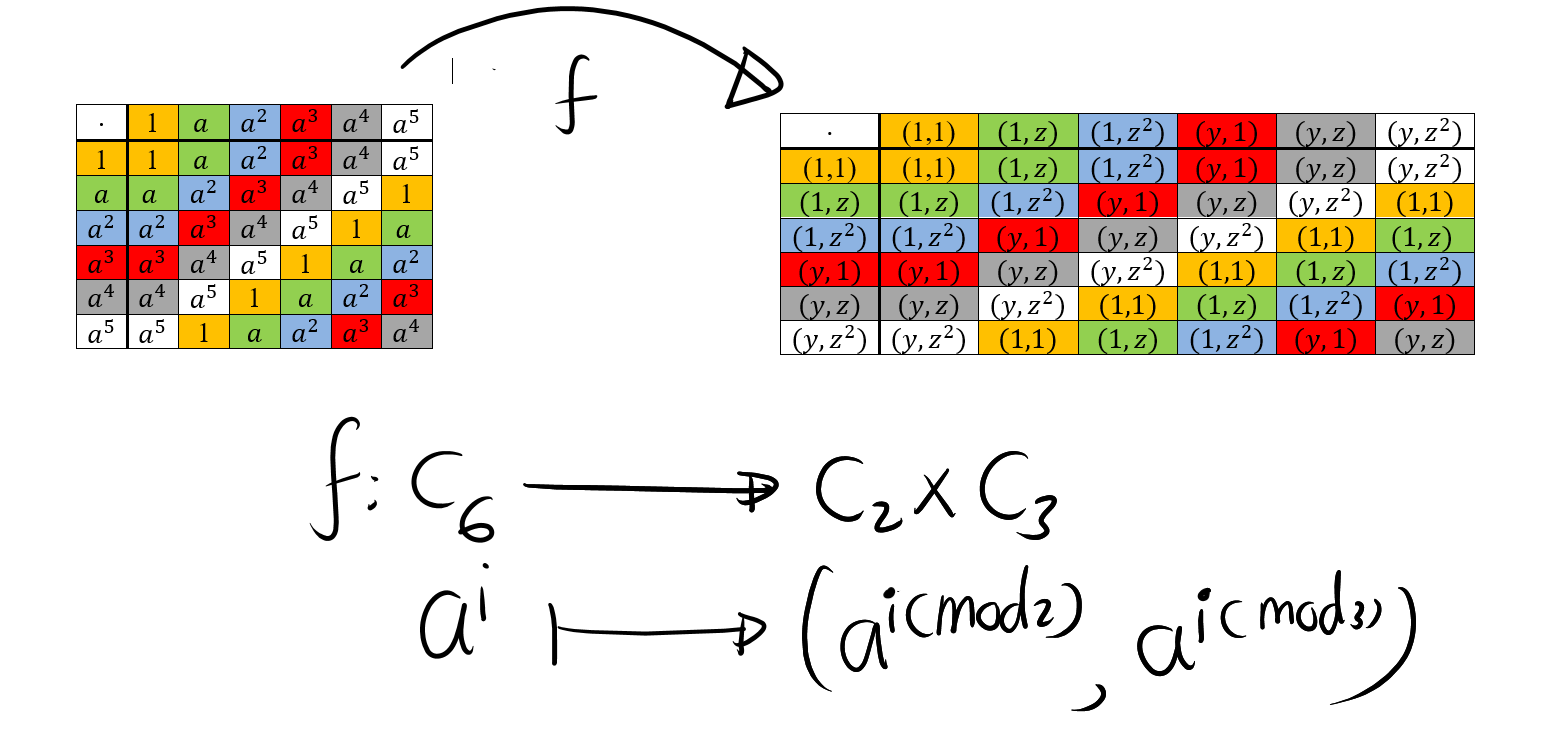
\includegraphics{figures/ch_2/fig02.png}
Here \(i=0,1,2...5\)

So let's try to see above result more generally.

\begin{proposition}
\protect\hypertarget{prp:unnamed-chunk-47}{}\label{prp:unnamed-chunk-47}Let \(r\) and \(s\) be relatively prime integers.
A cyclic group of order \(rs\) is isomorphic to the product of a cyclic group of order \(r\) and a cyclic group of order \(s\).
\end{proposition}

\begin{example}[s]
\protect\hypertarget{exm:unnamed-chunk-48}{}\label{exm:unnamed-chunk-48}On the other hand, a cyclic group of order \(4\) is not isomorphic to a product of two cyclic
groups of order \(2\).
\[C_4\not\equiv C2 \times C_2\]
Because , every element of \(C_2 \times C_2\) has order \(1\) or \(2\),whereasa cyclic group of order
\(4\) contains two elements of order \(4\).
\end{example}

The next proposition describes product groups.

\begin{proposition}
\protect\hypertarget{prp:prp2114}{}\label{prp:prp2114}Let \(G\) be a group and let \(H,K\leq G\), and let \(f: H \times K \rightarrow G\) be the multiplication map, defined by \(f(h, k) = hk\). Its image is the set \(HK = \{hk | h \in H, k \in K\}\).

\begin{enumerate}
\def\labelenumi{\alph{enumi}.}
\tightlist
\item
  \(f\) is injective if and only if \(H \cap K = \{1\}\).
\item
  \(f\) is a homomorphism from the product group \(H \times K\) to \(G\) if and only if elements of \(K\) commute with elements of \(H\): \(hk = kh\).
\item
  If \(H\) is a normal subgroup of \(G\), then \(HK\) is a subgroup of \(G\).
\item
  \(f\) is an isomorphism from the product group \(H \times K\) to \(G\) if and only if \(H \cap K = \{1\}\), \(HK = G\), and also \(H\) and \(K\) are normal subgroups of \(G\).
\end{enumerate}

It is important to note that the multiplication map may be bijective though it isn't a group homomorphism. This happens, for instance, when \(G = S_3\), and with the usual notation, \(H = \langle x \rangle\) and \(K = \langle y \rangle\).
\end{proposition}

\begin{proof}
\leavevmode

\begin{enumerate}
\def\labelenumi{\alph{enumi}.}
\tightlist
\item
\end{enumerate}

\begin{itemize}
\tightlist
\item
  (\(\Longrightarrow\)) We are going to use proof by contrapositive. So, suppose that \(x\in H\cap K\) such that \(x \neq 1\). Since \(x\in H\) then \(x^{-1} \in H\).
  \[f(x^{-1},x)=x^{-1}\cdot x=1=1\cdot 1=f(1,1)\]
  Thus, \(f\) is not injective. Thus, if \(f\) is injective then \(H \cap K = \{1\}\).
  -(\(\Longleftarrow\))
  Now Suppose that \(H \cap K = \{1\}\). Let \((h_1, k_1),(h_2, k_2)\in H \times K\) such that \(h_1k_1 = h_2k_2\). Now multiply both sides of this equation on the left by \(h_1^{-1}\) and on the right by \(k_2^{-1}\),
  \begin{eqnarray}
  h_1k_1 &=& h_2k_2\\
  h_1^{-1}(h_1k_1)k_2^{-1} &=& h_1^{-1}(h_2k_2)k_2^{-1}\\
  (h_1^{-1}h_1)k_1k_2^{-1} &=& h_1^{-1}h_2(k_2k_2^{-1})\\
  k_1k_2^{-1} &=& h_1^{-1}h_2
  \end{eqnarray}
  Note that \((k_1k_2^{-1})\in K\) and \(h_1^{-1}h_2\in H\). Since \(H \cap K = \{1\}\), \[k_1k_2^{-1} = h_1^{-1}h_2 = 1\]. Then,
  \[
  k_1=k_2~~\text{and}~~~~h_1=h_2.
  \]
  Then \[(h_1, k_1) = (h_2, k_2)\]
\end{itemize}

\begin{enumerate}
\def\labelenumi{\alph{enumi}.}
\setcounter{enumi}{1}
\tightlist
\item
  Let \((h_1, k_1),(h_2, k_2)\in H \times K\). Now consider,
  \begin{eqnarray}
  f((h_1,k_1)\cdot (h_2,k_2))&=&f((h_1h_2,k_1k_2))=h_1h_2k_1k_2\\
  f((h_1,k_1))\cdot f((h_2,k_2))&=& (h_1k_1)\cdot(h_2k_2)=h_1k_1h_2k_2
  \end{eqnarray}
\end{enumerate}

\begin{eqnarray}
f\text{ is homorphism} &\iff & 
f((h_1,k_1)\cdot (h_2,k_2))=f((h_1,k_1))\cdot f((h_2,k_2))\\
&\iff & h_1h_2k_1k_2=h_1k_1h_2k_2\\
&\iff & h_1^{-1}(h_1h_2k_1k_2)k_2^{-1}=h_1^{-1}(h_1k_1h_2k_2)k_2^{-1}\\
&\iff & (h_1^{-1}h_1)h_2k_1(k_2k_2^{-1})=(h_1^{-1}h_1)k_1h_2(k_2k_2^{-1})\\
&\iff & (h_1^{-1}h_1)h_2k_1(k_2k_2^{-1})=(h_1^{-1}h_1)k_1h_2(k_2k_2^{-1})\\
&\iff & h_2k_1=k_1h_2
\end{eqnarray}

\begin{enumerate}
\def\labelenumi{\alph{enumi}.}
\setcounter{enumi}{2}
\tightlist
\item
\end{enumerate}

\begin{itemize}
\item
  Suppose that \(H\) is a normal sub group of G. Note that \[KH=\bigcup_{k\in K}kH~~\text{   and     } ~~HK=\bigcup_{k\in K}Hk\]
  Since, \(H\) is normal, \(kH=Hk\) for all \(k\in K\). So, \(HK=KH\). We are going to use sub group test,

  \begin{itemize}
  \tightlist
  \item
    \emph{non-emptyness}: Clearly, \(1=1\cdot 1\in HK\) (because \(1\in H\) and \(1\in K\)
  \item
    \emph{closure}:
    \[HKHK=HHKK=HK\]
    Thus, \(HK\) is closed under multiplication.
  \item
    \emph{closed under inverse}: Let \(hk\in HK\). Then
    \[(hk)^{-1} = k^{-1}\cdot h^{-1} \in KH=HK \]
    This proves closure of \(HK\) under inverses.
  \end{itemize}
\end{itemize}

\begin{enumerate}
\def\labelenumi{\alph{enumi}.}
\setcounter{enumi}{3}
\tightlist
\item
\end{enumerate}

\begin{itemize}
\tightlist
\item
  \((\Longleftarrow)\): Suppose that \(H \cap K = \{1\}\), \(HK = G\), and also \(H,K \trianglelefteq G\). According to the (b), \(f\) is a homomorphism from \(H \times K\) to \(G\) if and only if \(hk = kh\) for all \(h\in H\). Consider,
  \[(hkh^{-1})k^{-1}=h(kh^{-1}k^{-1}).\]
  Note that, Since \(K \trianglelefteq G\), \(hkh^{-1}\in K\). So,\((hkh^{-1})k^{-1}\in K\). Similary we can show that \(h(kh^{-1}k^{-1})\in H\).Thus,\[(hkh^{-1})k^{-1}=h(kh^{-1}k^{-1})\in H\cap K.\] But from our hypothesis, \(H\cap K=\{1\}\). Hence,
\end{itemize}

\begin{eqnarray}
hkh^{-1}k^{-1}&=&1\\
hk&=& kh
\end{eqnarray}

Therefore, by (b) we can \(f\) is hormorphism. Now we have to proove bijectivity,
- \emph{Injectivity}: Already prooved in \ref{prp:prp2114} (a)
- \emph{Surjectivity}: For any \(g \in G\), we can write \(g = hk\) for some \(h \in H\) and \(k \in K\) (since \(Im(f)=HK = G\)). Thus, \(f(h, k) = hk = g\), so \(f\) is surjective.

Therefore \(f\) is an isomorphism.

\begin{itemize}
\item
  \((\Longrightarrow)\) Now suppose that \(f\) is isomorphism.

  \begin{itemize}
  \item
    \textbf{Claim i}: \(H \cap K = \{1\}\).\\
    Suppose that \(x\in H \cap K\). Then,
    \[f(1,x)=x=f(x,1)\]
    Since \(f\) is an isomorphism (and hence injective), we must have \(x = 1\). Therefore, \(H \cap K = \{1\}\).
  \item
    \textbf{Claim ii} :\(HK = G\).\\
    Since \(f\) is surjective, for any \(g \in G\), there exist \(h \in H\) and \(k \in K\) such that \(f(h, k) = hk = g\). Therefore, \(HK = G\).
  \item
    \textbf{Claim iii} : \(H\) and \(K\) are normal in \(G\).\\
    For any \(h \in H\) and \(g \in G\), we can write \(g = hk\) for some \(k \in K\). Then
    \[ghg^{-1} = (hk)h(hk)^{-1}
    =hk(hh^{-1})k^{-1}=h(kk^{-1})=h\in H.\]
    Thus, \(H\trianglelefteq G\).
    Similarly, we can show that \(K\trianglelefteq G\).
  \end{itemize}
\end{itemize}

\end{proof}

\hfill\break

\begin{proposition}
\protect\hypertarget{prp:unnamed-chunk-50}{}\label{prp:unnamed-chunk-50}There are two isomorphism classes of groups of order \(4\), the class of the cyclic group \(C_4\) of order \(4\) and the class of the Klein Four Group,which is isomorphic to the product \(C_2 \times C_2\) of two groups of order \(2\).
\end{proposition}

\begin{proof}
Let \(G\) be a group of order 4. The order of any element \(x\) of \(G\) divides 4, so there are two cases to consider:

\begin{itemize}
\tightlist
\item
  Case 1: \(G\) contains an element of order \(4 (|G|=4)\). Then \(G\) is a cyclic group of order \(4\).
\item
  Case 2: Every element of \(G\) except the identity has order \(2\).\\
  In this case, \(x = x^{-1}\) for every element \(x\) of \(G\). Let \(x\) and \(y\) be two elements of \(G\). Then \(xy\) has order \(2\), so \((xy)(x^{-1}y^{-1}) = (xy)(xy) = 1\). This shows that \(x\) and \(y\) commute,
\end{itemize}

\begin{eqnarray}
xyx^{-1}y^{-1} &=& 1\\
xyx^{-1}(y^{-1} y) &=& y\\
xyx^{-1} &=& y\\
xy(x^{-1}x) &=& yx\\
xy &=& yx
\end{eqnarray}

since \(x,y\) are arbitrary elements, \(G\) is abelian. So every subgroup is normal. We choose distinct elements \(x\) and \(y\) in \(G\), and we let \(H\) and \(K\) be the cyclic groups of order 2 that they generate. Proposition \ref{prp:prp2114} (d) shows that \(G\) is isomorphic to the product group \(H \times K\).
\end{proof}

\hypertarget{quotient-groups}{%
\section{Quotient Groups}\label{quotient-groups}}

\begin{definition}
\protect\hypertarget{def:unnamed-chunk-52}{}\label{def:unnamed-chunk-52}The set of cosets of a normal subgroup \(N\) of a group \(G\) is often denoted by \(G / N\).
\[G / N \text{ is the set of cosets of $N$ in} G\]
\end{definition}

\textbf{Notation}: When we regard a coset \(C\) as an element of the set of cosets, the bracket notation \([C]\)
may be used.
If \(C = aN\), we may also use the bar notation to denote the element \([C]\) by \(\overline{a}\),
and then we would denote the set of cosets by \(\overline{G}\):
\[\overline{G} = G /N\]

\begin{theorem}
\protect\hypertarget{thm:2122}{}\label{thm:2122}Let \(N\) be a normal subgroup of a group \(G\), and let \(G\) denote the set of cosets of \(N\) in \(G\). There is a law of composition on \(G\) that makes this set into a group, such that the map \(\pi: G \to \overline{G}\) defined by \(\pi(a) = \overline{a}\) is a surjective homomorphism whose kernel is \(N\).
\end{theorem}

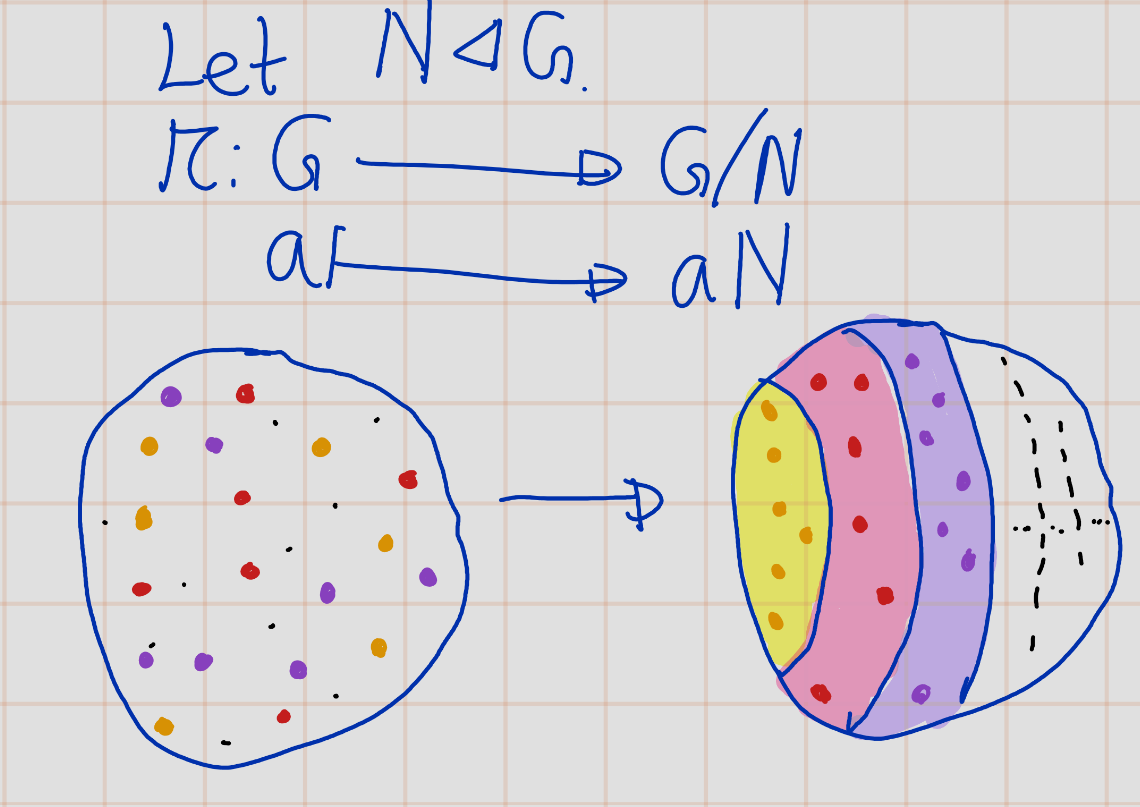
\includegraphics{figures/ch_2/fig29.png}

\begin{remark}
The map is often referred to as the canonical map from \(G\) to \(\overline{G}\). The word ``\textbf{canonical}''
indicates that this is the only map that we might reasonably be talking about
\end{remark}

The next corollary is very simple, but it is important enough to single out:

\begin{corollary}
\protect\hypertarget{cor:unnamed-chunk-54}{}\label{cor:unnamed-chunk-54}Let \(N \trianglelefteq G\), and let \(\overline{G}\) denote the set of cosets of \(N\) in \(G\). Let \(\pi: G \to \overline{G}=G/N\) be the canonical homomorphism. Let \(a_1, \ldots, a_k\in G\) such that the product \(a_1 \cdots a_k\in N\). Then \(\overline{a_1} \cdots \overline{a_k} = \overline{1}\).
\end{corollary}

\begin{proof}
Let \(p=a_1 \cdots a_k\in N\). This implies
\(\pi(p)=\overline{p}=\overline{1}\).\\
Since is \(pi\) a homomorphism, \(\pi(p)=\pi(a_1 \cdots a_k)=\pi(a_1)\cdots \pi(a_k)=\overline{a_1}\cdots\overline{a_n}\)
\end{proof}

\emph{Proof of \ref{thm:2122}}
There are several things to be done. We must

\begin{itemize}
\tightlist
\item
  define a law of composition on \(\overline{G}\),
\item
  prove that the law makes \(\overline{G}\) into a group,
\item
  prove that \(\pi\) is a surjective homomorphism, and
\item
  prove that the kernel of \(\pi\) is \(N\).
\end{itemize}

\begin{remark}

If \(A,B \subseteq G\) then \(AB\) denotes the set of products \(ab\):
\[AB:=\{x\in G: x=ab, a\in A, b\in B\}\]

\begin{itemize}
\tightlist
\item
  We will call this a product set, though in some other contexts the phrase ``product set'' refers
  to the set \(A \times B\) of pairs of elements
\end{itemize}

\end{remark}

\begin{lemma}
\protect\hypertarget{lem:2125}{}\label{lem:2125}Let \(N\) be a normal subgroup of a group \(G\), and let \(a N\) and \(b N\) be cosets of \(N\). The product set \((aN )(bN )\) is also a coset and \[(aN )(bN )=\{x\in G: x=anbn' ~\& ~ n,n'\in N\}=abN\].
\end{lemma}

\begin{proof}
Since \(N\) is a subgroup, \(N N = N\).\\
Since \(N\) is normal, left and right cosets are equal:
\(N b = bN\).
\[(aN )(bN ) = a (N b )N = a (b N )N = a b N N = abN\]
\end{proof}

\begin{itemize}
\tightlist
\item
  This lemma allows us to define multiplication on the set \(\overline{G} = G / N\).
\item
  Using the bracket
  notation, the definition is this: If \(C_1\) and \(C_2\) are cosets, then \([C_1][C_2] = [C_1 C_2]\),
  Where \(C_1 C_2\) is the product set.
\item
  The lemma shows that this product set is another coset.\\
\item
  To compute the product \([C_1][C_2]\), take any elements \(a \in C_1\) and \(b \in C_2\). Then \(C_1 = aN\) ,
  \(C_2 = bN\) , and \(C_1 C_2\) is the coset \(a b N\) that contains \(ab\). So,
  \[[aN][bN] = [abN] \text{ or } \overline{a}\overline{b} = \overline{ab}.\]
  Then by definition of the map \(\pi\) in theorm \ref{thm:2122},
  \[\pi(ab)=\overline{a}\overline{b} = \overline{ab}=\pi(a)\pi(b)\]
  The fact that \(\pi\) is a homomorphism will follow, once we show that G is a group.
  Since the canonical map \(\pi\) is surjective , the next lemma proves this
\end{itemize}

\begin{lemma}
\protect\hypertarget{lem:unnamed-chunk-58}{}\label{lem:unnamed-chunk-58}Let \(G\) be a group, and let \(Y\) be a set with a law of composition (both laws written with multiplicative notation). Consider a surjective map \(\varphi : G \to Y\) with the homomorphism property: \(\varphi(ab) = \varphi(a)\varphi(b)\) for all \(a\) and \(b\) in \(G\). Then \(Y\) is a group, and \(\varphi\) is a homomorphism.
\end{lemma}

\begin{proof}

The group axioms that are true in \(G\) are carried over to \(Y\) by the surjective map \(\varphi\).

\begin{itemize}
\item
  \textbf{Closure} : Let \(y_1,y_2\in Y\). Since \(\varphi\) is surjective, \(y_1=\varphi(x_1),y_2=\varphi(x_2)\) for some \(x_1,x_2\in G\).
  \[y_1y_2=\varphi(x_1)\varphi(x_2)=\varphi(x_1x_2)\in Y\]
\item
  \textbf{Assciativity Property} :\\
  Let \(y_1\), \(y_2\), and \(y_3\) be elements of \(Y\). Since \(\varphi\) is surjective, \(y_i = \varphi(x_i)\) for some \(x_i\) in \(G\). Then
\end{itemize}

\begin{eqnarray}
(y_1 y_2) y_3 &=& (\varphi(x_1) \varphi(x_2)) \varphi(x_3) = \varphi(x_1 x_2) \varphi(x_3) = \varphi((x_1 x_2) x_3) \\
&=^*& \varphi(x_1 (x_2 x_3)) = \varphi(x_1) \varphi(x_2 x_3) = y_1 (y_2 y_3)
\end{eqnarray}

The equality marked with an asterisk \((=^*)\) is the associative law in \(G\). The other equalities follow from the homomorphism property of \(\varphi\).

\begin{itemize}
\item
  \textbf{Identity}
  Let \(y\in Y\). Since \(\varphi\) is surjective, there exist \(x\in G\) such that \(y=\varphi(x)\). Let \(1_G\) be identity of \(G\) Then,
  \[y\varphi(1_G)=\varphi(x)\varphi(1_G)=\varphi(x1_G)=\varphi(x)=y=
    \varphi(1_Gx)=\varphi(1_G)\varphi(x)=\varphi(1_G)y\]
  Thus, \(\varphi(1_G)\) is the identity of \(Y\).
\item
  \textbf{Inverse} : Let \(y\in G\). Since \(\varphi\) is surjective, there exist \(x\in G\) such that \(y=\varphi(x)\),
  \[y\varphi(x^{-1}=\varphi(x)\varphi(x^{-1})
           =\varphi(xx^{-1})=\varphi(1_G)=\varphi(x^{-1}x)=\varphi(x^{-1})\varphi(x)=\varphi(x^{-1})y\]
  Thus, \(y^{-1}=\varphi(x)\)
\end{itemize}

\end{proof}

The only thing remaining to be verified is that the kernel of the homomorphism \(\pi\) is the subgroup \(N\).

\begin{eqnarray}
\pi (a) =\pi(1) &\iff & \bar{a}= \bar{1}\\
& \iff & [aN] = [1N]\\
& \iff & a \in N.
\end{eqnarray}
Thus, \(\ker(\pi)=N\)

\begin{figure}
\centering
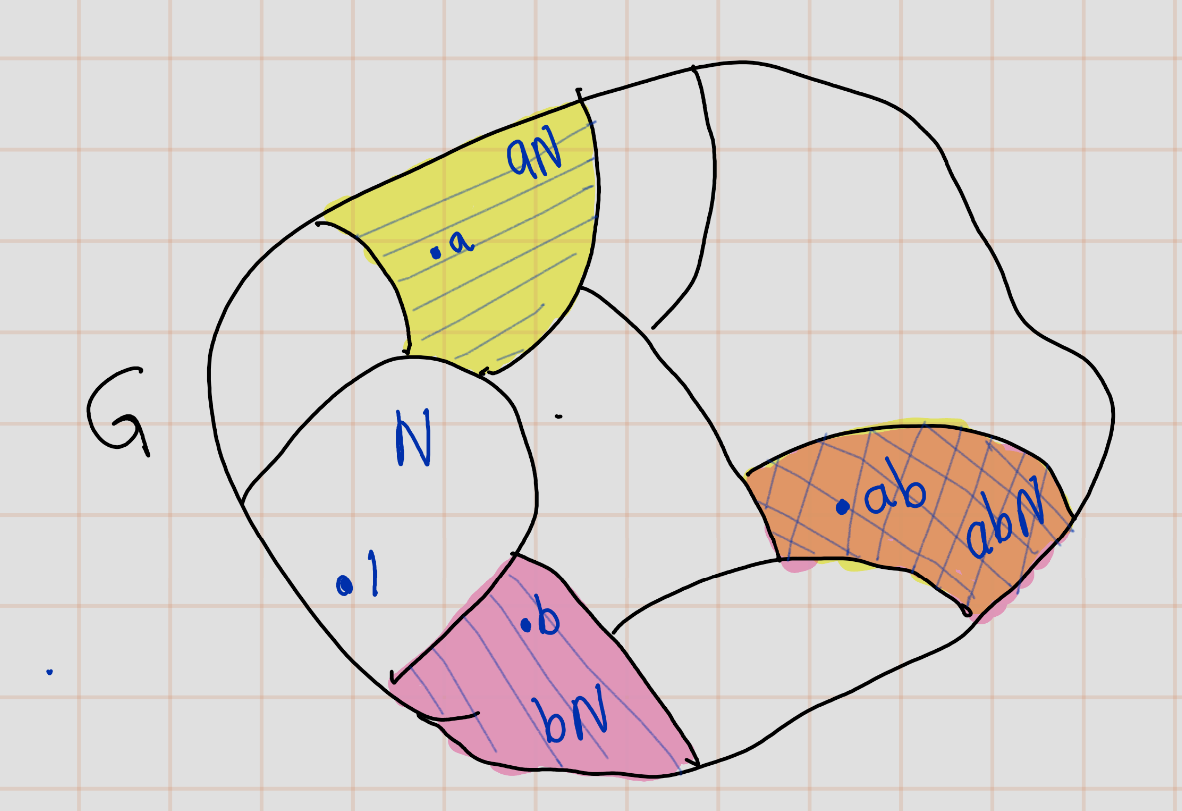
\includegraphics{figures/ch_2/fig30.png}
\caption{\label{fig:fig2-30}A Schematic Diagram of Coset Multiplication.}
\end{figure}

\begin{remark}
Our assumption that \(N\) is a \textbf{normal} subgroup of \(G\) is crucial to lemma \ref{lem:2125}. If \(H\) is \textbf{not} normal, there will be left cosets \(C_1\) and \(C_2\) of \(H\) in \(G\) such that the product set \(C_1 C_2\) does not lie in a single left cosets.

Let's see an example for this. Going back once more to the subgroup \(H = \langle y \rangle\) of \(S_3\).
Note that the subgroup \(H\) is not normal.\\
The product set \((1H)(xH)\) contains four elements: \[(1H)(xH)=\{1, y\}\{x, xy\} = \{x, xy, x^2y, x^2\}\]. It is not a coset.
\end{remark}

The next theorem relates the quotient group construction to a general group homomorphism, and it provides a fundamental method of identifying quotient groups.

\begin{theorem}[First Isomorphism Theorem]
\protect\hypertarget{thm:unnamed-chunk-61}{}\label{thm:unnamed-chunk-61}Let \(\varphi: G \to G'\) be a surjective group homomorphism with kernel \(N\). The quotient group \(\overline{G}=G/N\) is isomorphic to the image \(G'\). To be precise, let \(\pi: G \to \overline{G}=G/N\) be the canonical map. There exists a unique isomorphism \(\overline{\varphi}: G/N \to G'\) such that \(\varphi = \psi \circ \pi\).
\end{theorem}

\begin{center}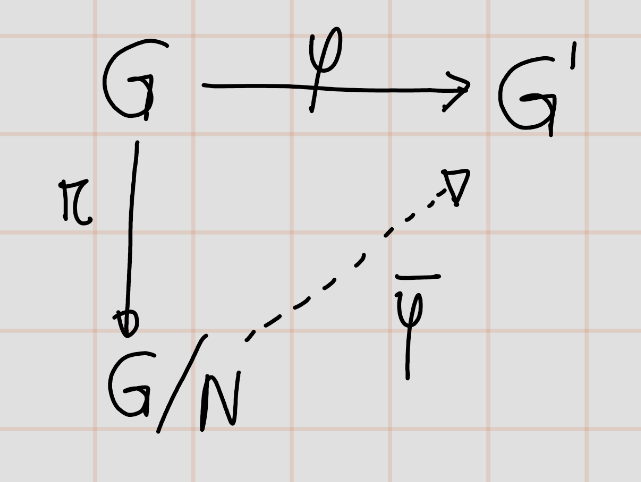
\includegraphics[width=0.5\linewidth]{figures/ch_2/fig31} \end{center}

\begin{proof}
The elements of \(\overline{G}=G/N\) are the cosets of \(N\), and they are also the fibres of the map \(\varphi\). The map \(\overline{\varphi}\) referred to in the theorem is the one that sends a non-empty fibre to its image: \(\overline{\varphi}(\overline{x})=\varphi(x)\). For any surjective map of sets \(\varphi: G \to G'\), one can form the set \(\overline{G}\) of fibres, and then one obtains a diagram as above, in which \(\overline{\phi}\) is the bijective map that sends a fibre to its image. When \(\phi\) is a group homomorphism, \(\overline{\phi}\) is an isomorphism because
\[\overline{\phi}(\overline{ab}) = \phi(ab) = \phi(a)\phi(b) = \overline{\phi}(\overline{a})\overline{\phi}(\overline{b}).\]
\end{proof}

\hfill\break

\begin{corollary}
\protect\hypertarget{cor:unnamed-chunk-63}{}\label{cor:unnamed-chunk-63}Let \(\varphi: G \rightarrow G'\) be a group homomorphism with kernel \(N\) and image \(H'\). The quotient group \(\overline{G}=G/N\) is isomorphic to the image \(H'\).
\end{corollary}

\hypertarget{lienaer-operators}{%
\chapter{Lienaer Operators}\label{lienaer-operators}}

\hypertarget{exercises}{%
\chapter{Exercises}\label{exercises}}

\hypertarget{chapter-2}{%
\section{Chapter 2}\label{chapter-2}}

\hypertarget{laws-of-composition}{%
\subsection{Laws of composition}\label{laws-of-composition}}

\begin{exercise}[Artin 2.1.1]
\protect\hypertarget{exr:unnamed-chunk-64}{}\label{exr:unnamed-chunk-64}Let \(S\) be a set. Prove that the law of composition defined by \(ab = a\) for all \(a\) and \(b\) in \(S\) is associative? For which sets does this law have an identity?
\end{exercise}

\textbf{Solution}: Let \(a,b,c\in S\).
Now consider following
\[(ab)c=(ac)=a=(ab)=a(bc)\]
Thus, the given law of composition is associative.

If the given law of composition has an identity element whenever every element \(a\in S\) has a multiplicative inverse./
In other words, for every element \(a\in S\), there exists an element \(e \in S\) such that \[ae = ea = a.\]
Thus, \(ae=a=ea=e\). So, the identity element is the same as every element in S, and the law has an identity for all sets S. Thus, only singletons sets have this given law of compositions have identity.

\begin{exercise}[Artin 2.1.2]
\protect\hypertarget{exr:unnamed-chunk-65}{}\label{exr:unnamed-chunk-65}Prove the properties of inversesthat are listed near the end ofthe section.
\end{exercise}

\begin{itemize}
\tightlist
\item
  If an element \(a\) has both a left inverse \(l\) and a right inverse \(r\), then \(r = l\), \(a\) is invertible and \(r\) is its inverse.
\end{itemize}

\begin{proof}
Since \(l\) is a left inverse for \(a\), then \(la = 1\). In the same way, since \(r\) is a right inverse for \(a\) the equality \(ar = 1\) holds. Let us now consider the expression \(lar\). By associativity of the composition law in a group we have \(r = 1r = (la)r = lar = l(ar) = l1 = l\). This implies that \(l = r\). Since \(l = r\), it holds also that that \(ar = 1 = la = ra\) hence \(a\) is invertible and \(r\) is its inverse.
\end{proof}

\begin{itemize}
\tightlist
\item
  If \(a\) is invertible, its inverse is unique.
\end{itemize}

\begin{proof}
Let \(i_1\) and \(i_2\) be inverses of \(a\). In particular \(i_1\) is a left inverse of \(a\) and \(i_2\) is a right inverse of \(a\). By point (a) \(i_1 = i_2\).
\end{proof}

\begin{itemize}
\tightlist
\item
  Inverses multiply in the opposite order: if \(a\) and \(b\) are invertible, then the product \(ab\) is invertible and \((ab)^{-1} = b^{-1}a^{-1}\).
\end{itemize}

\begin{proof}
In order to show that \(ab\) is invertible, it is enough to exhibit an element that is a right and a left inverse of \(ab\). The element \(b^{-1}a^{-1}\) is a right inverse of \(ab\) since \(abb^{-1}a^{-1} = a(bb^{-1})a^{-1} = a1a^{-1} = aa^{-1} = 1\). It is a left inverse since \(b^{-1}a^{-1}ab = b^{-1}(a^{-1}a)b = b^{-11}b = b^{-1}b = 1\). This proves that \(ab\) is invertible and that \(b^{-1}a^{-1}\) is its inverse.
\end{proof}

\hypertarget{groups-and-subgroups-1}{%
\subsection{Groups and Subgroups}\label{groups-and-subgroups-1}}

\begin{exercise}[Artin 2.2.1]
\protect\hypertarget{exr:unnamed-chunk-69}{}\label{exr:unnamed-chunk-69}Make a multiplication table for the symmetric group \(S_3\).
\end{exercise}

\textbf{Solution}

\begin{longtable}[]{@{}lllllll@{}}
\toprule\noalign{}
\(\circ\) & \textbf{e} & (12) & (13) & (23) & (123) & (132) \\
\midrule\noalign{}
\endhead
\bottomrule\noalign{}
\endlastfoot
\textbf{e} & e & (12) & (13) & (23) & (123) & (132) \\
\textbf{(12)} & (12) & e & (123) & (132) & (13) & (23) \\
\textbf{(13)} & (13) & (123) & e & (132) & (23) & (12) \\
\textbf{(23)} & (23) & (132) & (123) & e & (12) & (13) \\
\textbf{(123)} & (123) & (13) & (23) & (12) & (132) & e \\
\textbf{(132)} & (132) & (23) & (12) & (13) & e & (123) \\
\end{longtable}

\begin{exercise}[Artin 2.2.2]
\protect\hypertarget{exr:unnamed-chunk-70}{}\label{exr:unnamed-chunk-70}Let \(S\) be a se t with an associative law of composition and with an identity element. Prove that the subset consisting of the invertible elements in \(S\) is a group.
\end{exercise}

\begin{proof}
Let \(S^*\subseteq S\) with consisting of the invertible elements in \(S\).

\begin{itemize}
\item
  \emph{identity} : We are given identity element \(1 \in S\) and \((1^{-1})(1)=1 \implies 1 \in S^*\).
\item
  \emph{Closure} :
  So let \(a,b\in S^*\). Then \(a,b\) are invertible. Let \(a^{-1},b^{-1}\in S^*\) be inverses of \(a\) and \(b\) respectively. Now we need to check \(ab\in S^*\).\\
\end{itemize}

\[(b^{-1}a^{-1})(ab)=b^{-1}(a^{-1}a)b=b^{-1}b=e=
  aa^{-1}=a(bb^{-1})a^{-1}=(ab)(b^{-1}a^{-1})\]
\end{proof}

Thus, \((ab)^{-1}=b^{-1}a^{-1}\). So, \(ab\in S^*\)
Therefore, \(S^*\) is closed under the composition.

\begin{itemize}
\tightlist
\item
  \emph{Associativity}: The associativity property inherit from the group \(S\).
\end{itemize}

Therefore, \(S^*\) is a group.

\begin{exercise}[Artin 2.2.3]
\protect\hypertarget{exr:unnamed-chunk-72}{}\label{exr:unnamed-chunk-72}

Let \(G\) be a group.Let \(x, y, z,w \in G\).

\begin{enumerate}
\def\labelenumi{(\alph{enumi})}
\tightlist
\item
  Solve for \(y\), given that \(xyz^{-1}w = 1\).
\item
  Suppose that \(xyz = 1\). Does it follow that \(yzx = 1\)? Does it follow that \(yxz = 1\)?
\end{enumerate}

\end{exercise}

\textbf{Solution}:

\begin{enumerate}
\def\labelenumi{\alph{enumi}.}
\tightlist
\item
  \hfill\break
  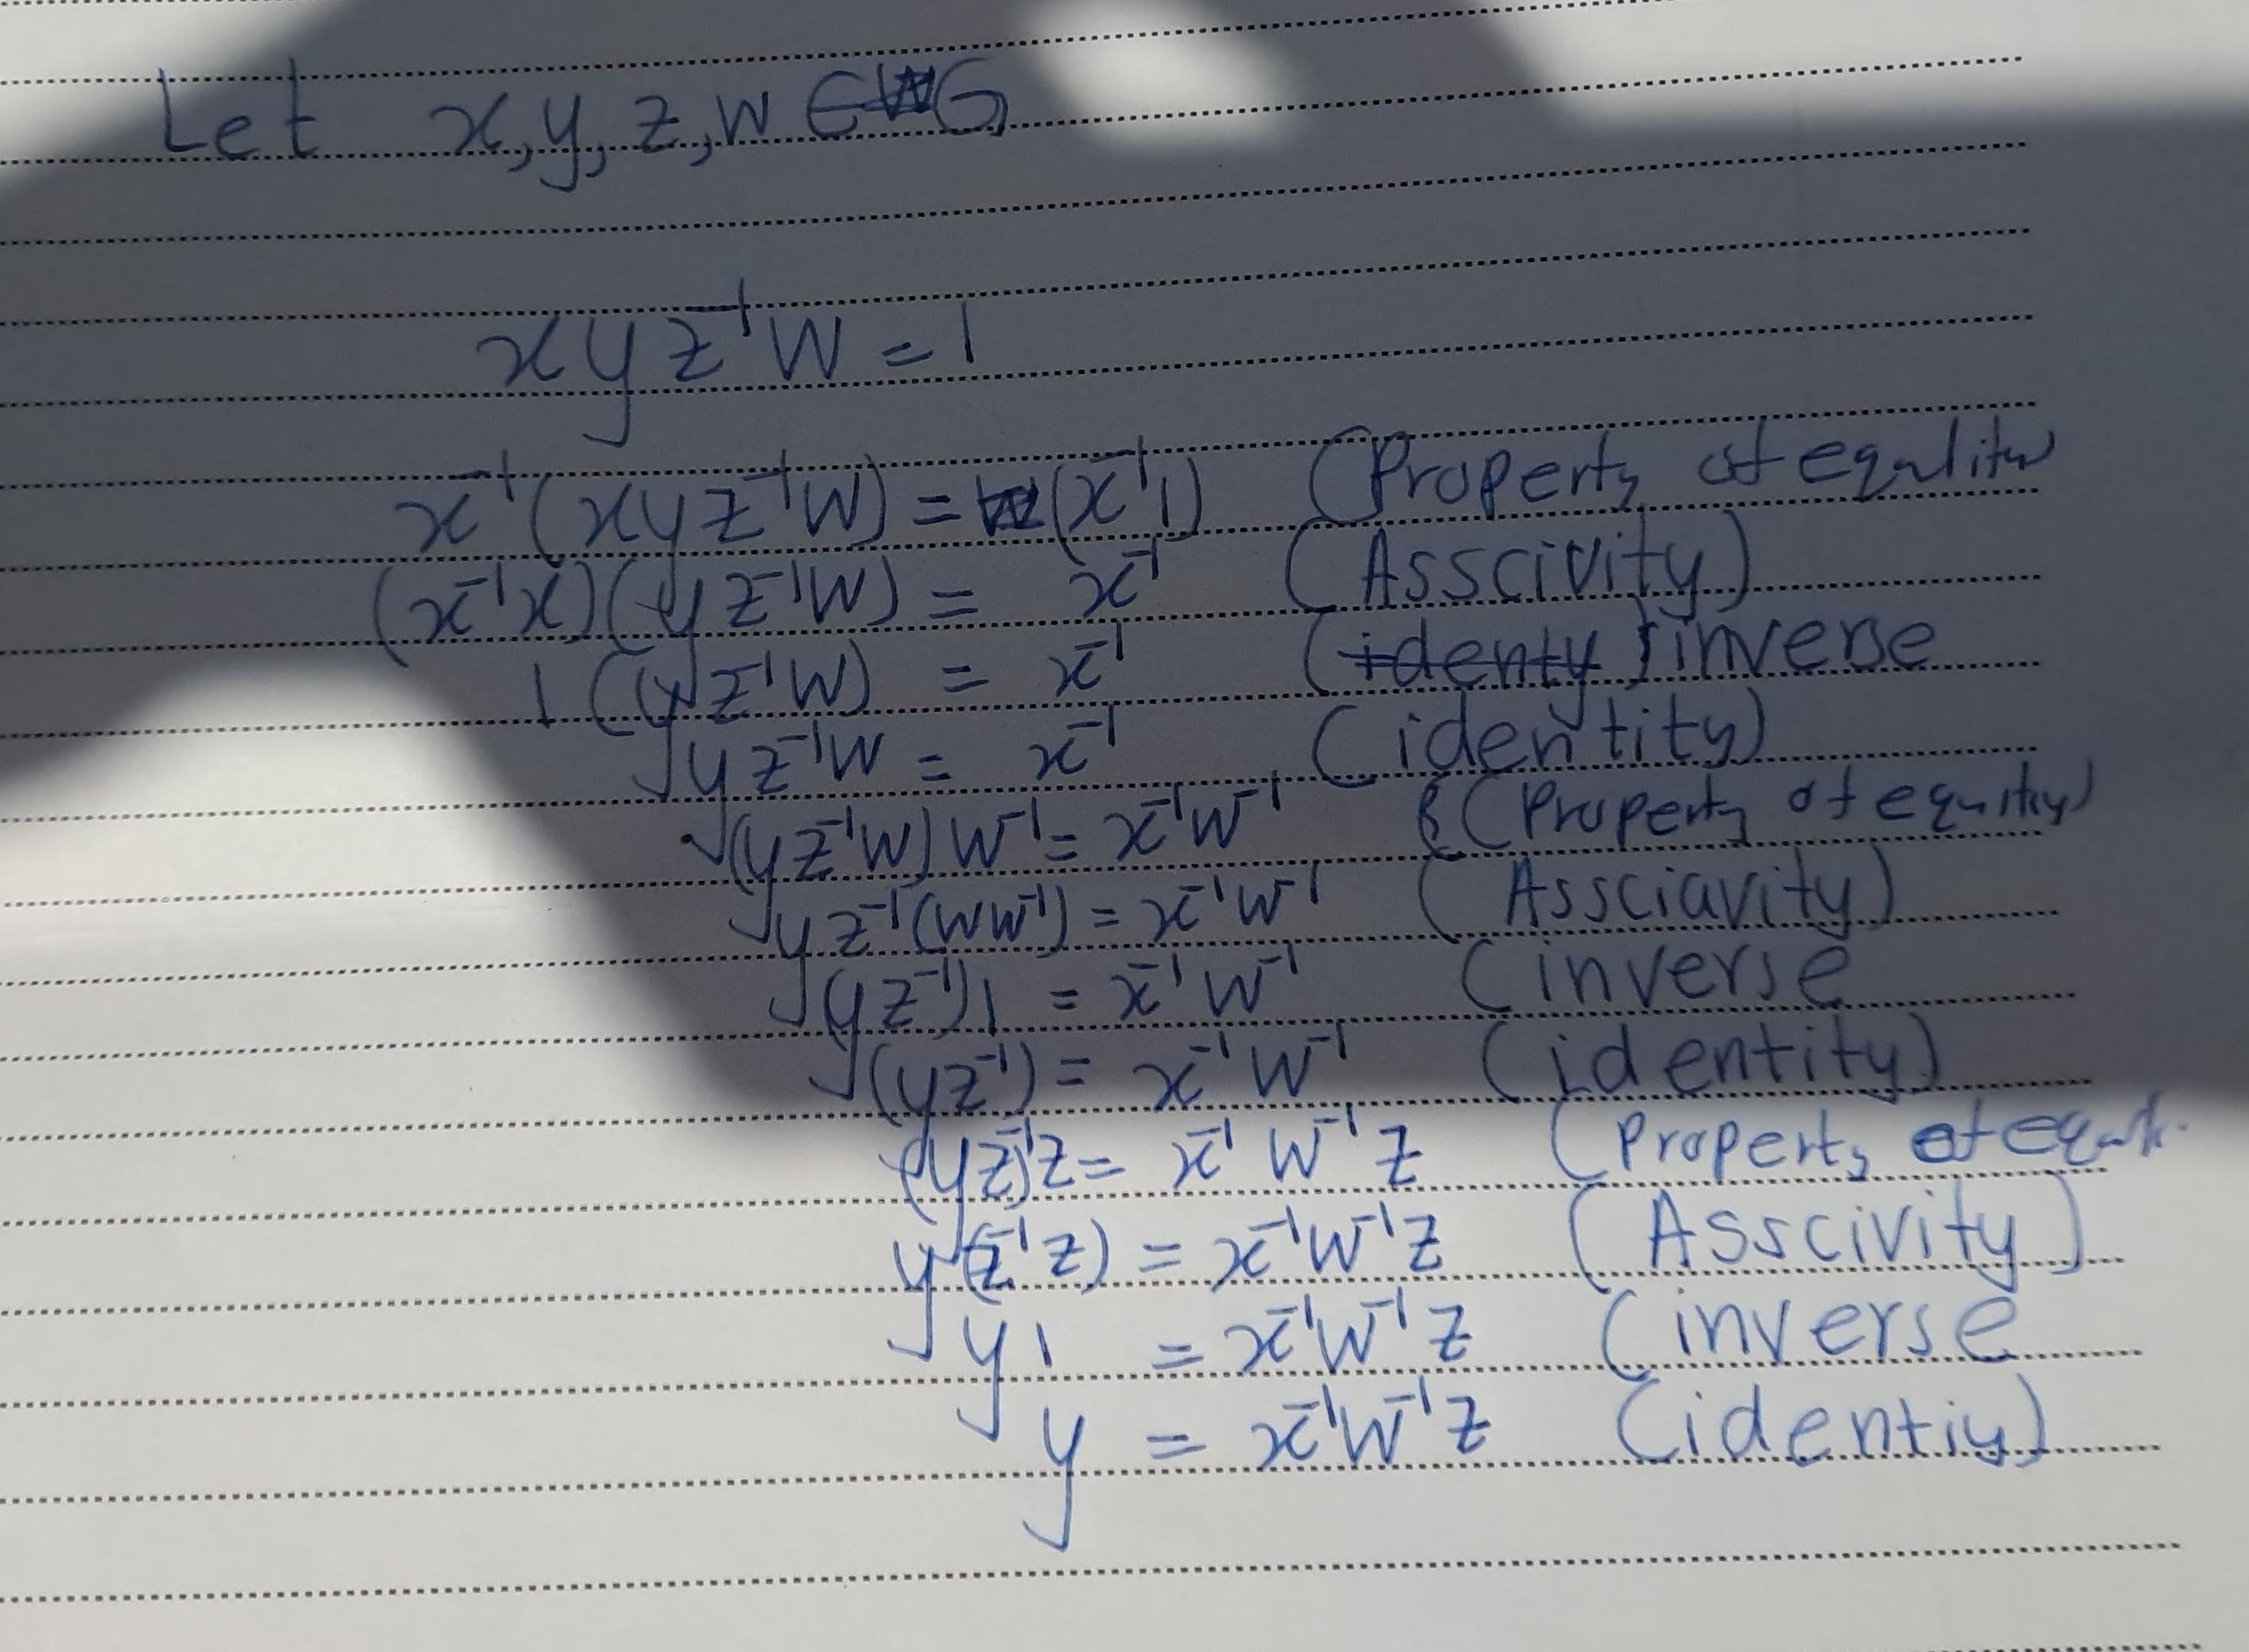
\includegraphics{figures/ch_2/fig17.jpg}
\item
  \hfill\break
\end{enumerate}

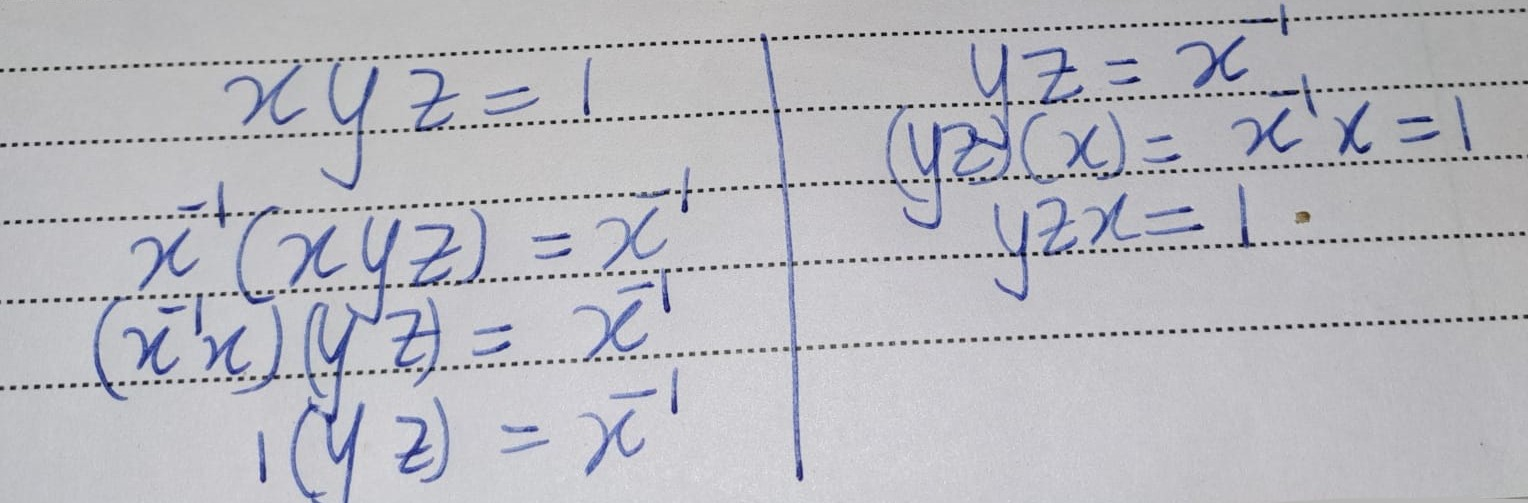
\includegraphics{figures/ch_2/fig18.jpg}
- The given statement is false.
\begin{eqnarray}
          xyz&=&1\\
  x^{-1}(xyz)&=&x^{-1} \cdot 1\\
  (x^{-1}x)(yz)&=&x^{-1}\\
  1 \cdot(yz)&=&x^{-1}\\
  (yz)&=&x^{-1}\\
  (yz)z^{-1}&=&x^{-1}z^{-1}\\
  y(zz^{-1})&=&x^{-1}z^{-1}\\
  y \cdot 1&=&x^{-1}z^{-1}\\
  yx&=&x^{-1}z^{-1}x\\
  yxz&=&x^{-1}z^{-1}xz\\
\end{eqnarray}
If \(G\) is not abelian or \(z\neq x\). \(xyz=1 \nRightarrow yxz=1\).

\begin{exercise}[Artin 2.2.4]
\protect\hypertarget{exr:unnamed-chunk-73}{}\label{exr:unnamed-chunk-73}

In which of the following cases is \(H\) a subgroup of \(G\)?

\begin{enumerate}
\def\labelenumi{(\alph{enumi})}
\item
  \(G = GL_n(\mathbb{C})\) and \(H = GL_n(\mathbb{R})\).
\item
  \(G = \mathbb{R}^\times\) and \(H = \{1, -1\}\).
\item
  \(G = \mathbb{Z}^+\) and \(H\) is the set of positive integers.
\item
  \(G = \mathbb{R}^+\) and \(H\) is the set of positive reals.
\item
  \(G = GL_2(\mathbb{R})\) and \(H\) is the set of matrices \(\begin{bmatrix} a & 0 \\ 0 & 0 \end{bmatrix}\) with all entries equal to 0.
\end{enumerate}

\end{exercise}

\textbf{Solution}:\\

\begin{enumerate}
\def\labelenumi{(\alph{enumi})}
\tightlist
\item
\end{enumerate}

\begin{itemize}
\item
  \emph{Subset ?} : Since every matrix with real entries can be interpreted as a matrix with complex entries, we conclude that \(H \subset G\).
\item
  \emph{Closure ?} : For every \(A, B \in GL_n(\mathbb{R})\) we have \(AB \in GL_n(\mathbb{R})\) since Product of invertible matrices is invertible. I proved this result in chapter 1.
\item
  \emph{Identity ?} :The identity in \(G\) is \(I_n\), the identity \(n x n\) matrix. Observe that \(I_n\in H=GL_n(\mathbb{R})\). (Because every entry of \(I_n\) is 1 or 0)
\item
  \emph{Inverse ?}: \(GL_n(\mathbb{R})\) is the set of \(n \times n\) invertible matrices with real entries. So, all the elements in \(H\) is invertible.
\end{itemize}

Therefore, \(H \leq G\)

\begin{enumerate}
\def\labelenumi{(\alph{enumi})}
\setcounter{enumi}{1}
\tightlist
\item
\end{enumerate}

\begin{itemize}
\item
  \emph{Subset ?} : This is trivial \(\{-1,1\}\subset \mathbb{R}^\times\)
\item
  \emph{Closure ?} :
\end{itemize}

\begin{eqnarray}
1 \times 1 &=& 1\in H\\
(-1) \times 1 &=& (-1)\in H\\
1 \times (-1) &=& (-1)\in H\\
(-1) \times (-1) &=& -1\in H\\
\end{eqnarray}
Thus, \(H\) is closed.
- \emph{Identity ?} : The identity in \(G\) is \(1\), which is also in \(H\).

\begin{itemize}
\tightlist
\item
  \emph{Inverse ?} :
  \begin{eqnarray}
  1 \times 1 = 1   &\implies & (1)^{-1}=1\in H\\
  (-1) \times (-1) = 1 &\implies & (-1)^{-1}=(-1)\in H
  \end{eqnarray}
  x`Therefore, \(H\) is sub group of \(G\).
\end{itemize}

\begin{enumerate}
\def\labelenumi{(\alph{enumi})}
\setcounter{enumi}{2}
\item
  Note that \(2\in H\), but inverse of \(2\) in \(\mathbb{Z}^+\) is \((-2) \not \in H\).\\
  Therefore, \(H\) is not a subgroup of \(G\).
\item
\end{enumerate}

\begin{itemize}
\item
  \emph{Subset ?} : This is trivial. \(H \subset \mathbb{R}^\times\)
\item
  \emph{Closure ?} : Product of positive real number is positive. Thus, \(H\) is closed.
\item
  \emph{Identity ?} : \(1\) is the identity of \(G\), which is in \(H\).
\item
  \emph{Inverse ?} : Let \(a\in H\). Then,
  \[a\cdot \frac{1}{a}=\frac{1}{a}\cdot a=1\]
  So, \(\frac{1}{a}\in H\) is the inverse of \(a\). Thus, \(H\) is closed under inverses.
\end{itemize}

\begin{enumerate}
\def\labelenumi{(\alph{enumi})}
\setcounter{enumi}{4}
\tightlist
\item
  Let \(A=\begin{bmatrix} 2 & 0 \\ 0 & 0 \end{bmatrix}\) Then \(A\in H\). But observe that \(det(A)=0\implies A\) is not invertible. Thus, \(A\not\in H\). Thus, this \(H \not\subseteq G\).
\end{enumerate}

Therefore, \(H\) is not a subgroup of \(G\).

\begin{exercise}[Artin 2.2.5]
\protect\hypertarget{exr:unnamed-chunk-74}{}\label{exr:unnamed-chunk-74}

In the definition of a subgroup, the identity element in \(H\) is required to be the identity
of \(G\). One might require only that H have an identity element, not that it need be the
same as the identity in \(G\).

\begin{itemize}
\tightlist
\item
  Show that if \(H\) has an identity at all, then it is the identity in \(G\).
\item
  Show that the analogous statement is true for inverses.
\end{itemize}

\end{exercise}

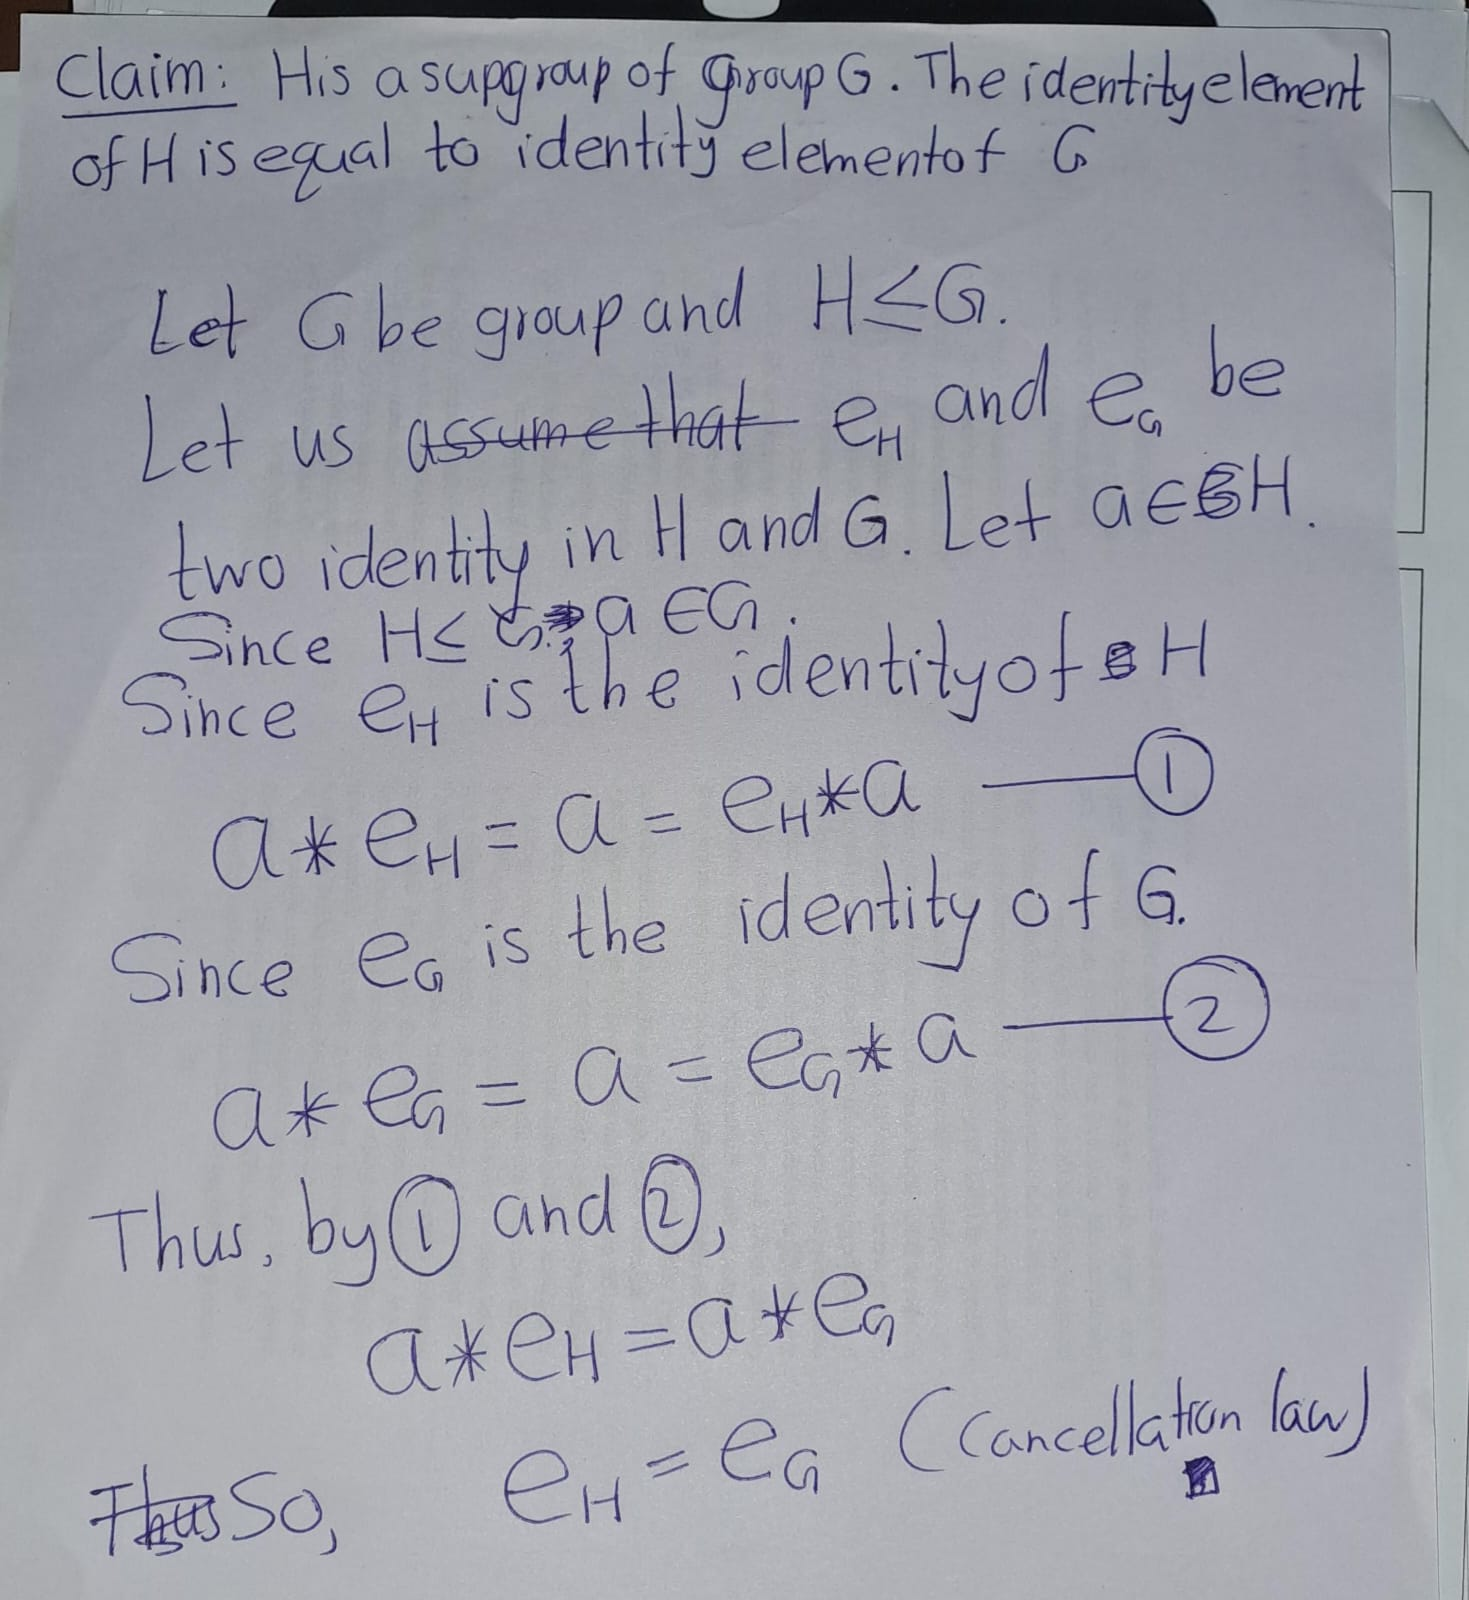
\includegraphics{figures/ch_2/fig49.jpg}
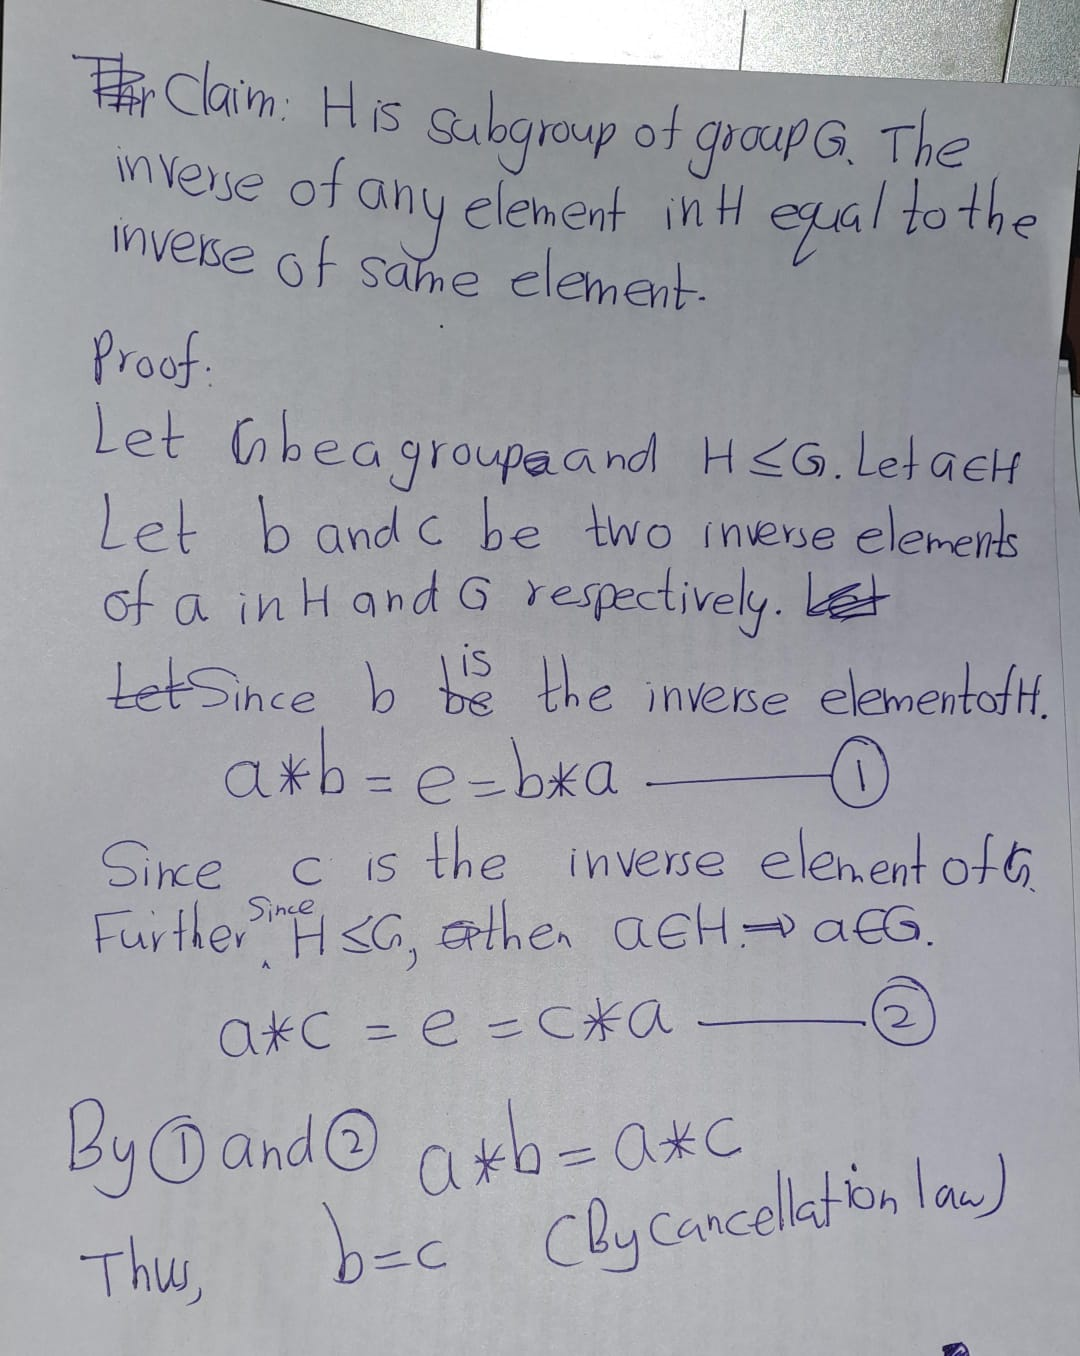
\includegraphics{figures/ch_2/fig50.jpg}

\begin{exercise}[Artin 2.2.6]
\protect\hypertarget{exr:unnamed-chunk-77}{}\label{exr:unnamed-chunk-77}Let \(G\) be a group. We define an opposite group \(G^{\circ}\) with the law of composition \(a * b\) as follows:
- The underlying set is the same as \(G\),
- but the law of composition is \(a * b = ba\).

Prove that \(G^{\circ}\) is a group.
\end{exercise}

\textbf{Solution}:

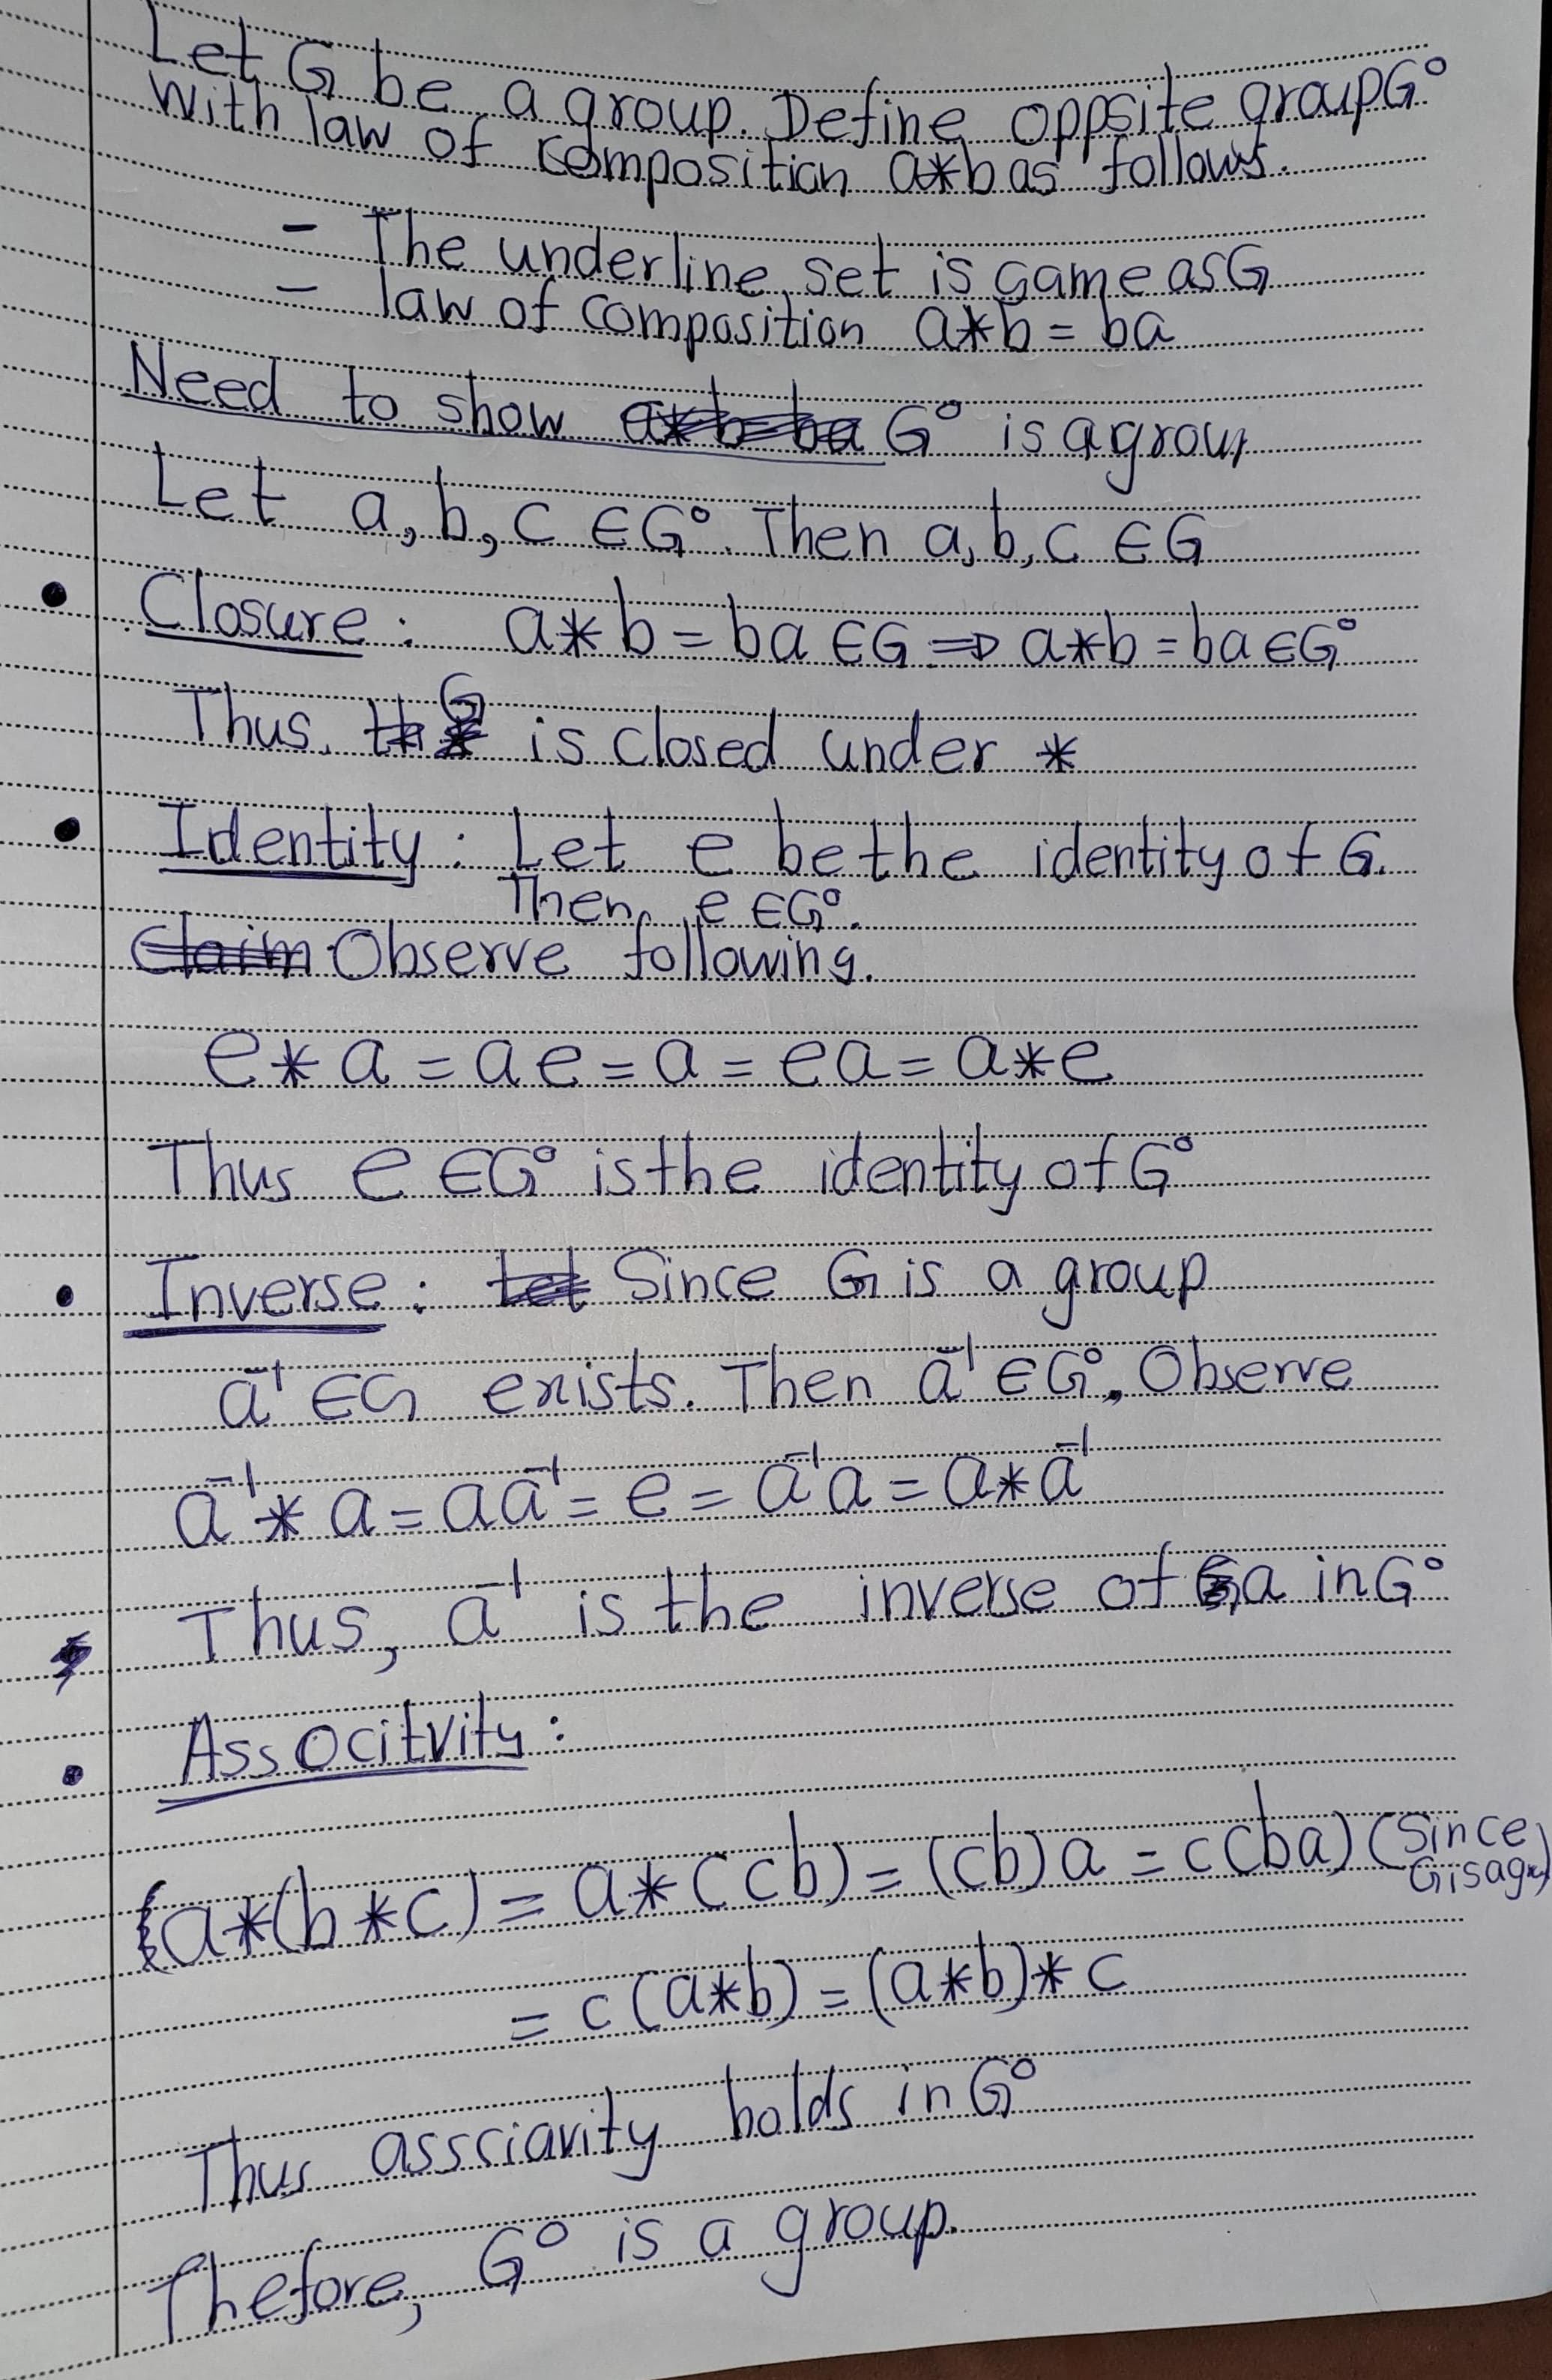
\includegraphics{figures/ch_2/fig19.jpg}

\hypertarget{subgroups-of-the-additive-group-of-integers-1}{%
\subsection{Subgroups of the Additive Group of Integers}\label{subgroups-of-the-additive-group-of-integers-1}}

\begin{exercise}[Artin 2.3.1]
\protect\hypertarget{exr:unnamed-chunk-78}{}\label{exr:unnamed-chunk-78}Let \(a = 123\) and \(b = 321\).
Compute \(d = gcd(a, b)\), and express \(d\) as an integer
combination \(ra + bs\).
\end{exercise}

\textbf{Solution}:
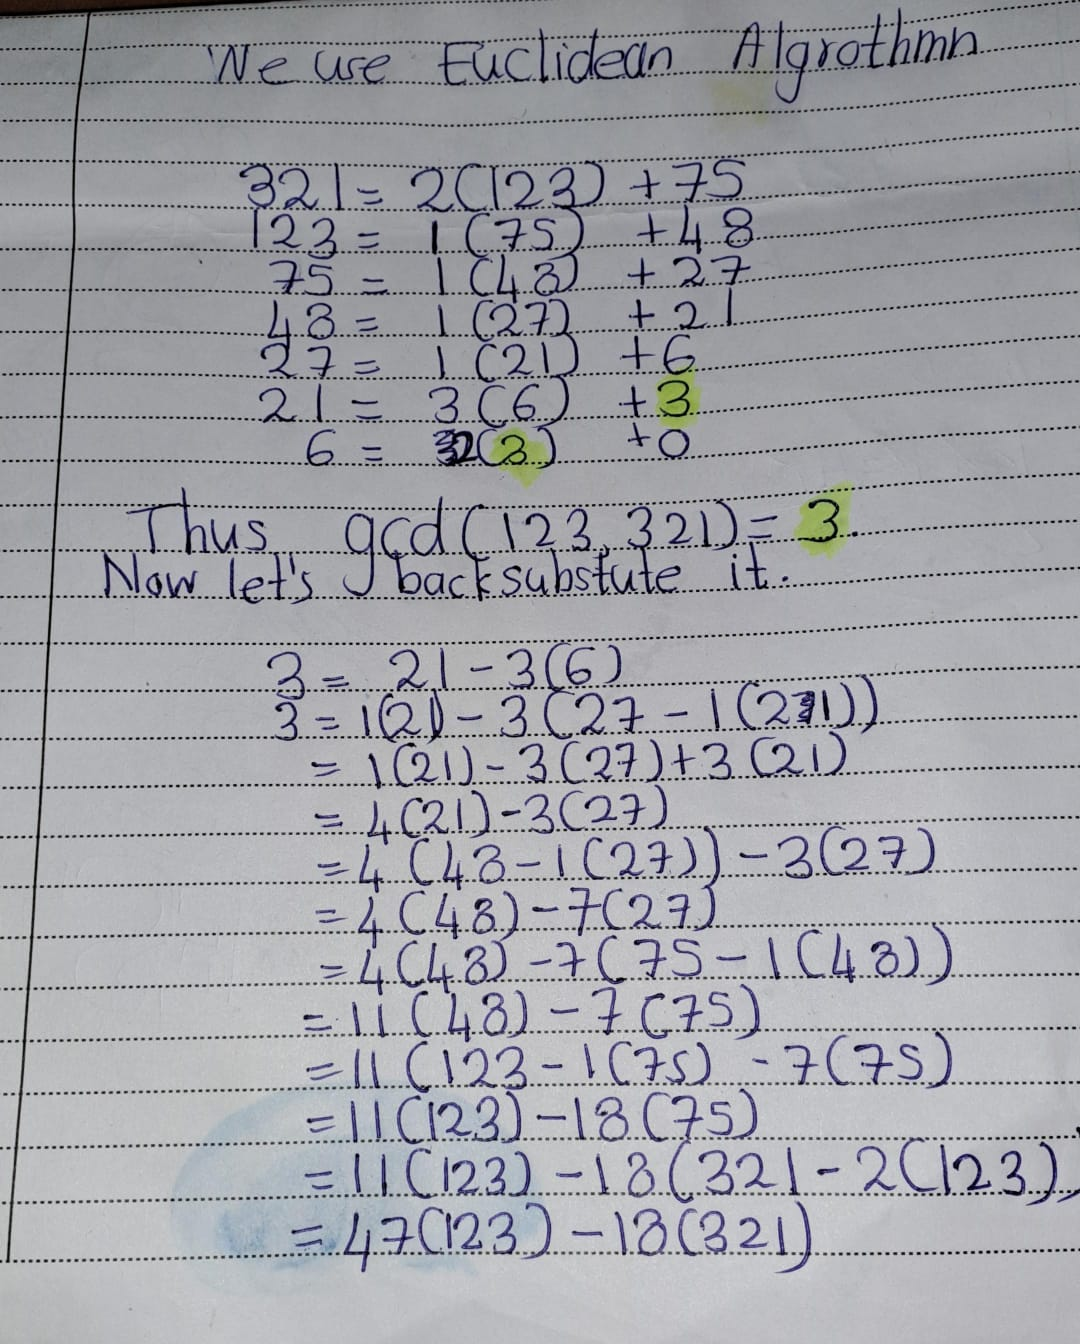
\includegraphics{figures/ch_2/fig20.jpg}

\begin{exercise}[Artin 2.3.2]
\protect\hypertarget{exr:unnamed-chunk-79}{}\label{exr:unnamed-chunk-79}Prove that if \(a\) and \(b\) are positive integers whose sum is a prime \(p\), their greatest common
divisor is \(1\).
\end{exercise}

\textbf{Solution}:
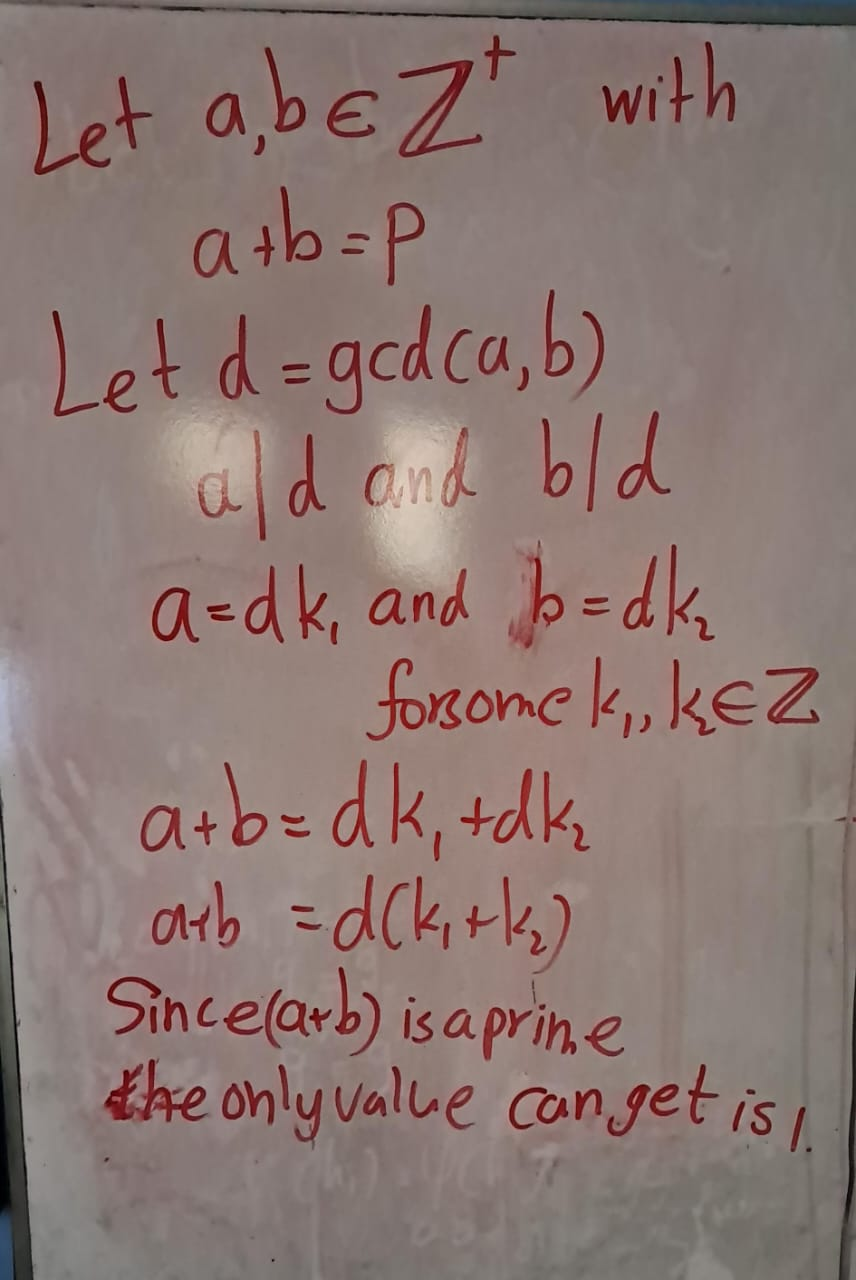
\includegraphics{figures/ch_2/fig21.jpg}

\begin{exercise}[Artin 2.3.3]
\protect\hypertarget{exr:unnamed-chunk-80}{}\label{exr:unnamed-chunk-80}\leavevmode

\begin{enumerate}
\def\labelenumi{\alph{enumi}.}
\tightlist
\item
  Define the greatest common divisor of a set \(\{a_1, ..., a_n\}\) of \(n\) integers. Prove that it exists, and that it is an integer combination of \(a_1, ..., a_n\).
\item
  Prove that if the greatest common divisor of \(\{a_1, ..., a_n\}\) is \(d\), then the greatest common divisor of \(\{a_1/d, ..., a_n/d)\) is \(1\).
\end{enumerate}

\end{exercise}

\textbf{Solution}:

\begin{enumerate}
\def\labelenumi{\alph{enumi}.}
\tightlist
\item
\end{enumerate}

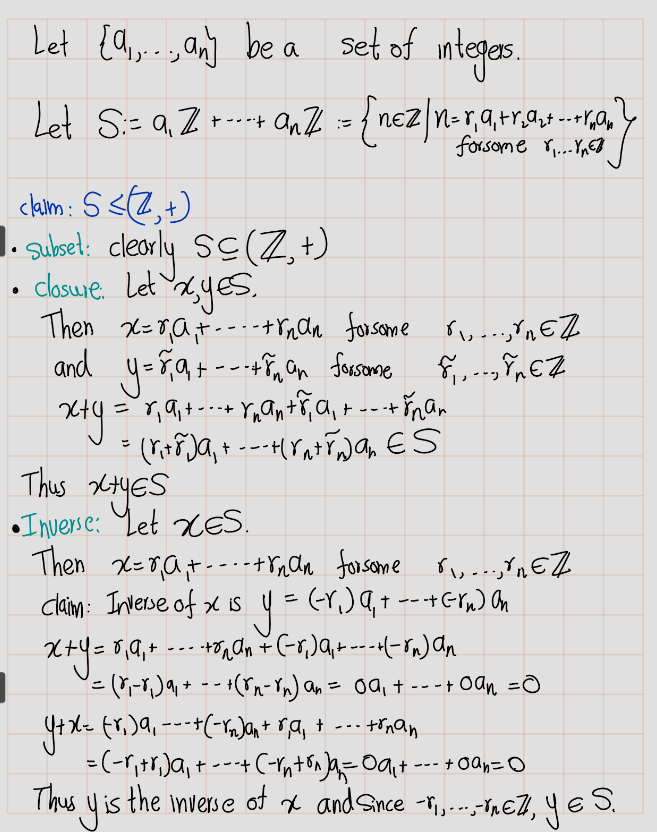
\includegraphics{figures/ch_2/fig51.png}
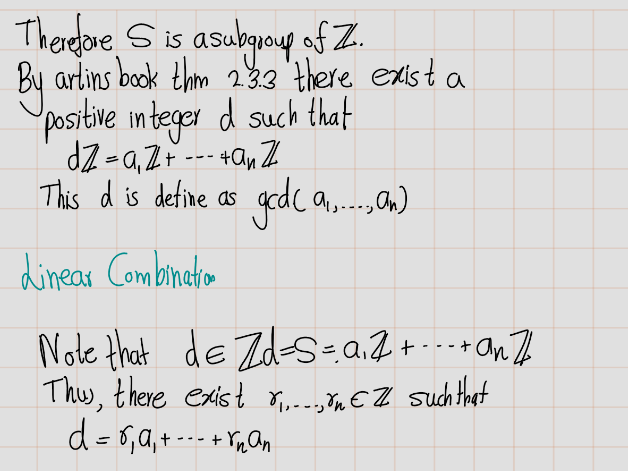
\includegraphics{figures/ch_2/fig52.png}
b.

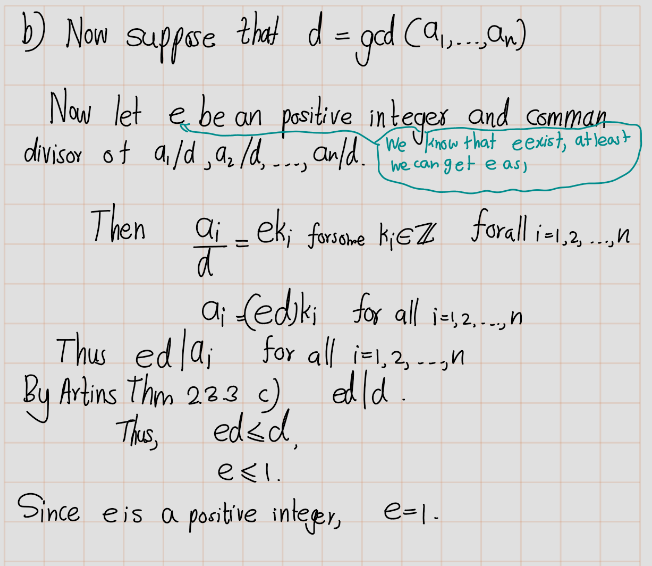
\includegraphics{figures/ch_2/fig53.png}

\hypertarget{cyclic-group}{%
\subsection{Cyclic group}\label{cyclic-group}}

\begin{exercise}[Artin 2.4.1]
\protect\hypertarget{exr:unnamed-chunk-84}{}\label{exr:unnamed-chunk-84}Let \(a\) and \(b\) be elements of a group \(G\). Assume that a has order \(7\) and that \(a^3b = ba^3\).
Prove that \(a b = ba\).
\end{exercise}

\textbf{Solution}:

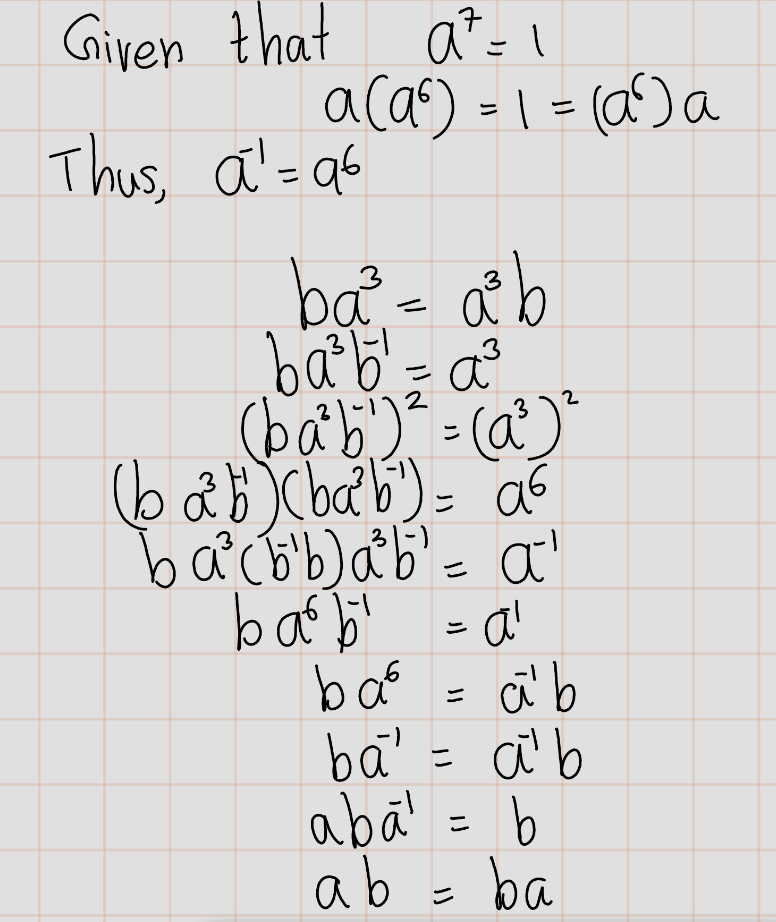
\includegraphics{figures/ch_2/fig22.png}

\begin{exercise}[Artin 2.4.2]
\protect\hypertarget{exr:unnamed-chunk-85}{}\label{exr:unnamed-chunk-85}

An \(n\)th root of unity is a complex number \(z\) such that \(z^n = 1\).

\begin{enumerate}
\def\labelenumi{(\alph{enumi})}
\tightlist
\item
  Prove that the nth roots of unity form a cyclic subgroup of \(\mathbb{C}^\times\) of order \(n\).
\item
  Determine the product of all the \(n\)th roots of unity.
\end{enumerate}

\end{exercise}

\textbf{Solution}:
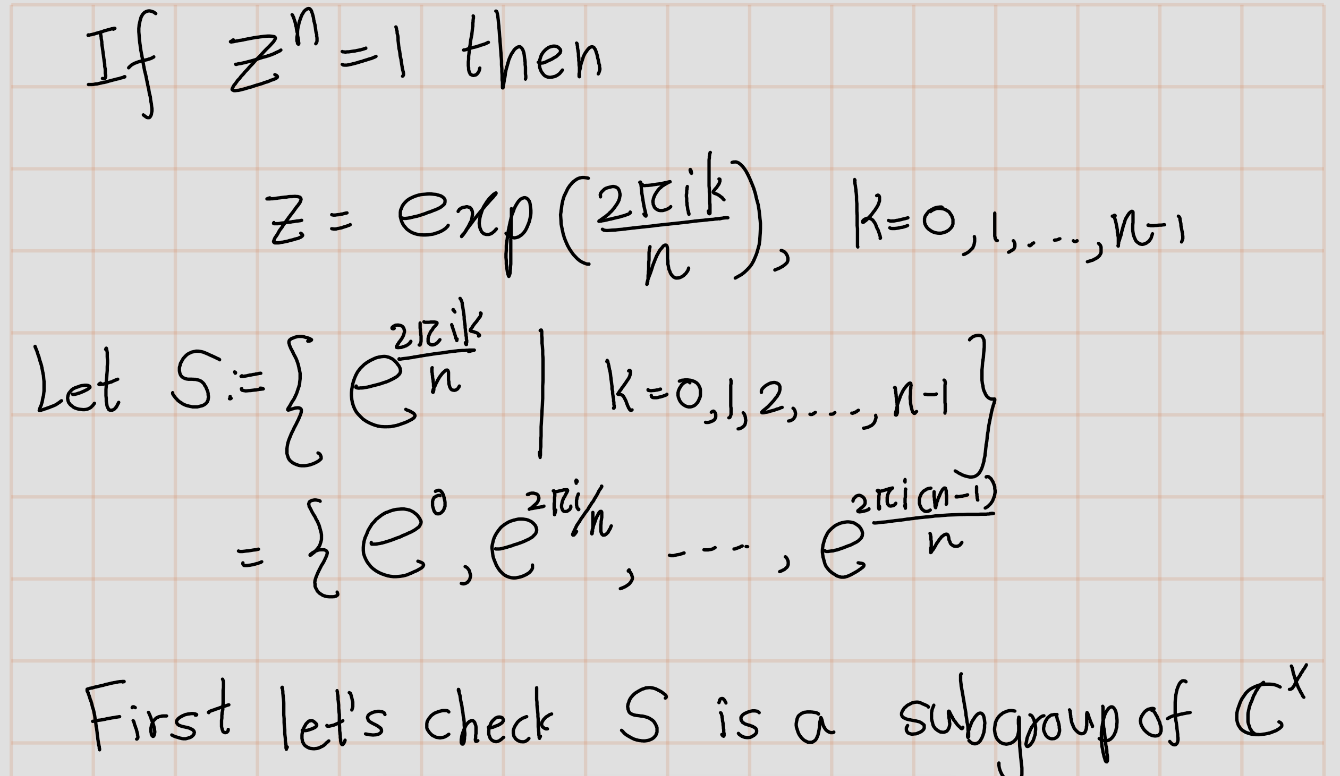
\includegraphics{figures/ch_2/fig23.png}

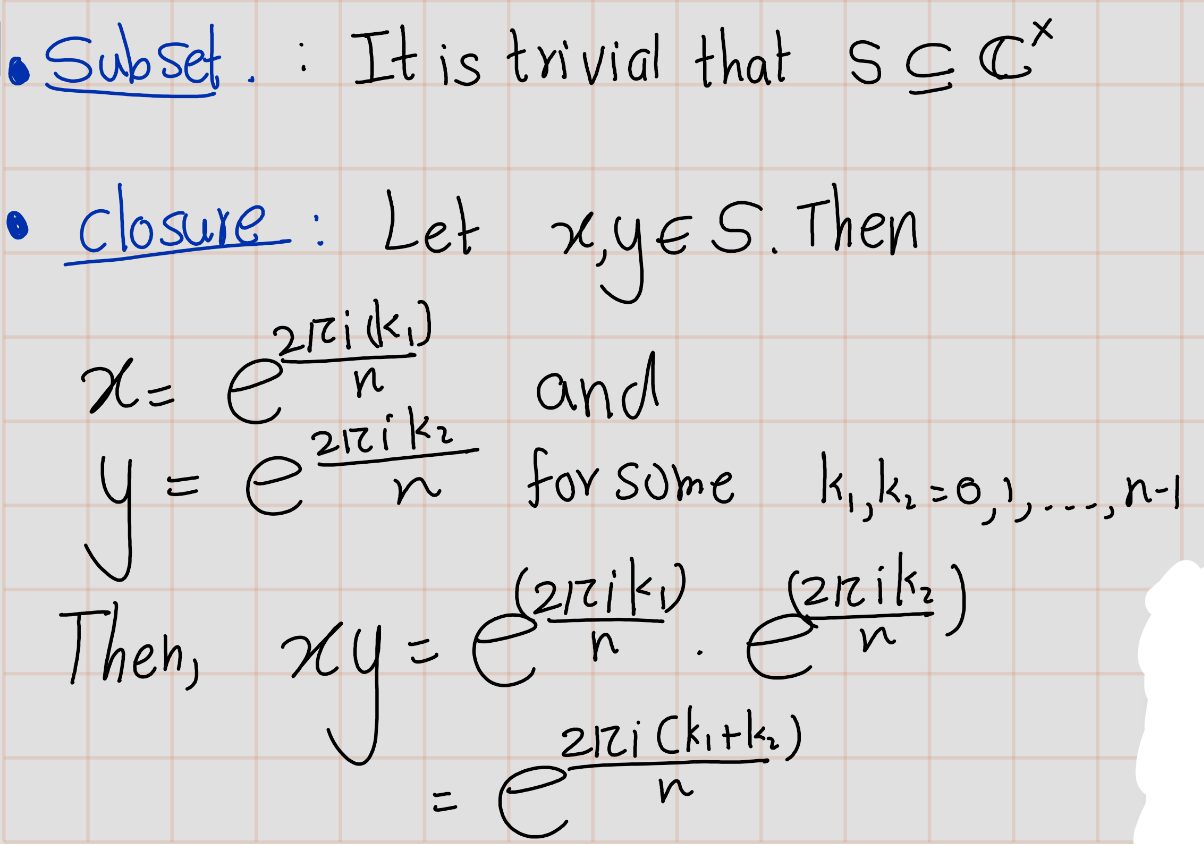
\includegraphics{figures/ch_2/fig24.png}

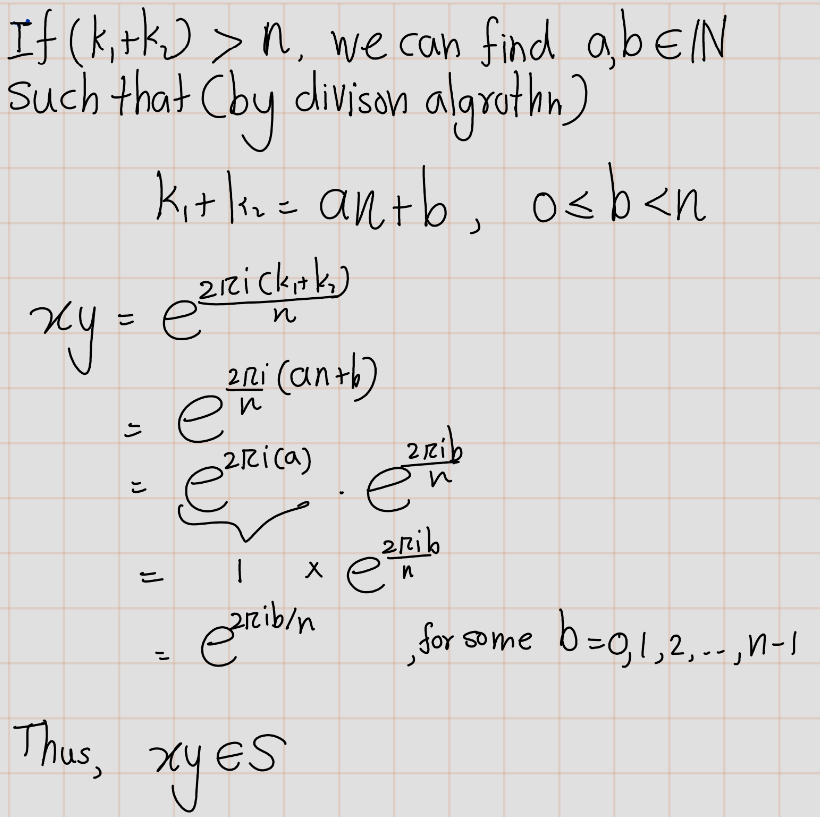
\includegraphics{figures/ch_2/fig25.png}
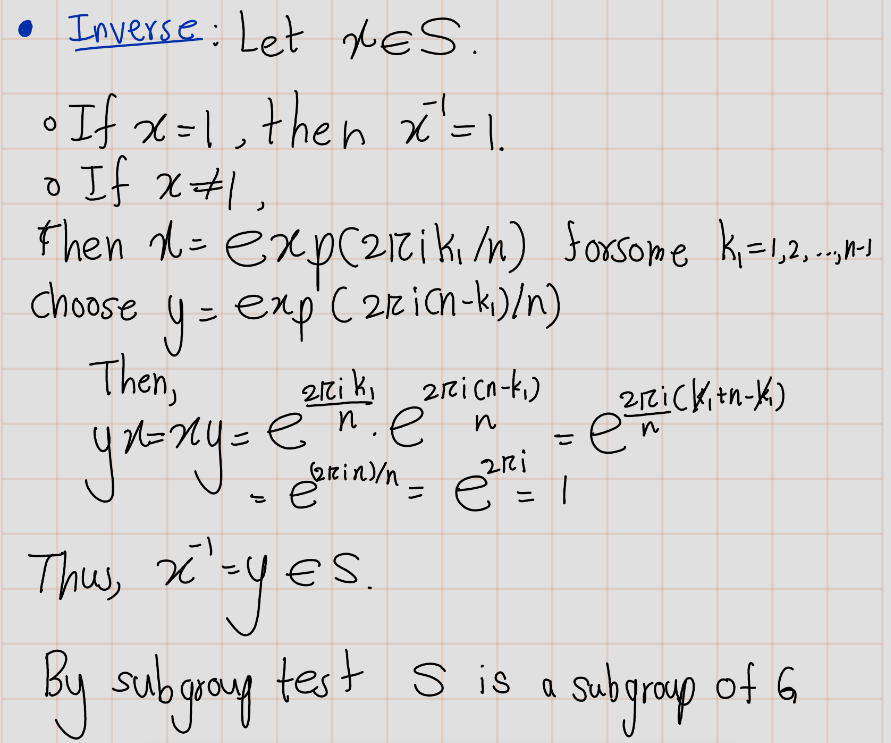
\includegraphics{figures/ch_2/fig26.png}
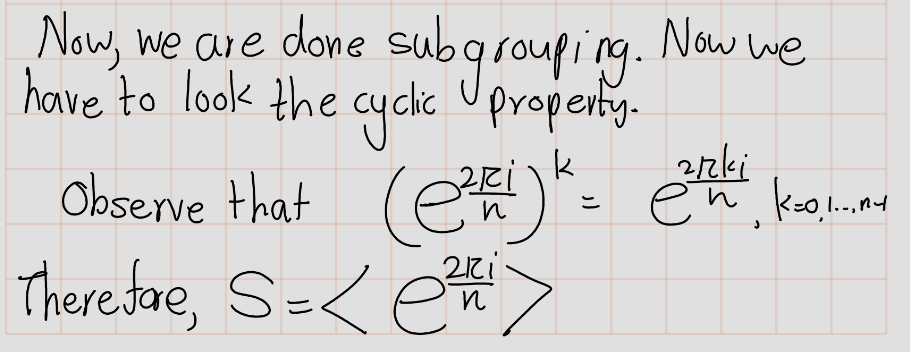
\includegraphics{figures/ch_2/fig27.png}
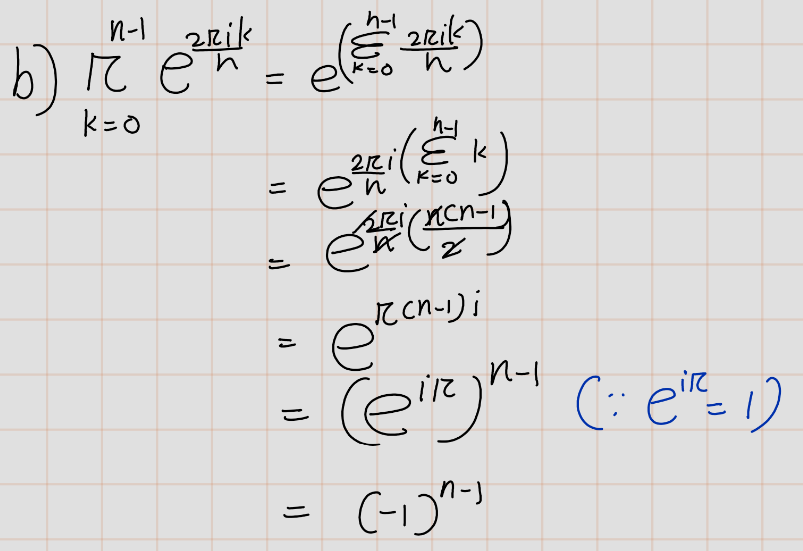
\includegraphics{figures/ch_2/fig28.png}

\begin{exercise}[Artin 2.4.3]
\protect\hypertarget{exr:unnamed-chunk-86}{}\label{exr:unnamed-chunk-86}Let \(a\) and \(b\) be elements of a group \(G\). Prove that \(ab\) and \(ba\) have the same order
\end{exercise}

\begin{proof}
Let \(a\) and \(b\) be elements in a group \(G\) with identity \(e\).

Suppose that \(ab\) has finite order \(n\). Then \((ab)^n = e\) and \(n\) is the smallest positive integer for which this equation is true. We also have that \[ (ba)^{n+1} = (ba)(ba) \cdots (ba) = b\underbrace{(ab) \cdots (ab)}_{n \text{ times}}a =b(ab)^na=a(ba)^m b =bea = ba. \]

Thus, since \((ba)^{n+1} = (ba)^n(ba)\) we can conclude that \((ba)^n(ba) = ba\) and then by the cancellation law, we have that \((ba)^n = e.\)

Now, to show that the order of \(ba\) is \(n\), we need to demonstrate that \(n\) is the smallest positive integer such that \((ba\)\^{}n = e. )

Suppose there exists a positive integer \(m < n\) such that \((ba)^m = e.\)
Then,\[
(ab)^{m+1} =(ab)(ab)\cdots(ab)=a\underbrace{(ba)\cdots(ba)}_{m \text{ times}}b=a(ba)^m b=aeb= ab.
\]

Thus, since\((ab)^{m+1} =(ab)^m(ab)\)
we have that
\((ab)^m(ab)= ab\)
and then by the cancellation law, we have that
\((ab)^m=e\)
which contradicts the fact that \(n\) is the smallest positive integer such that
\((ab)^n=e.\)

Hence, \(n\) is the smallest positive integer such that
\((ba)^n=e\)
and therefore
\((ba)\) has finite order \(n\).
\end{proof}

\begin{exercise}[Artin 2.4.4]
\protect\hypertarget{exr:unnamed-chunk-88}{}\label{exr:unnamed-chunk-88}Describe all groups G that contain no proper subgroup
\end{exercise}

\textbf{Solution}:
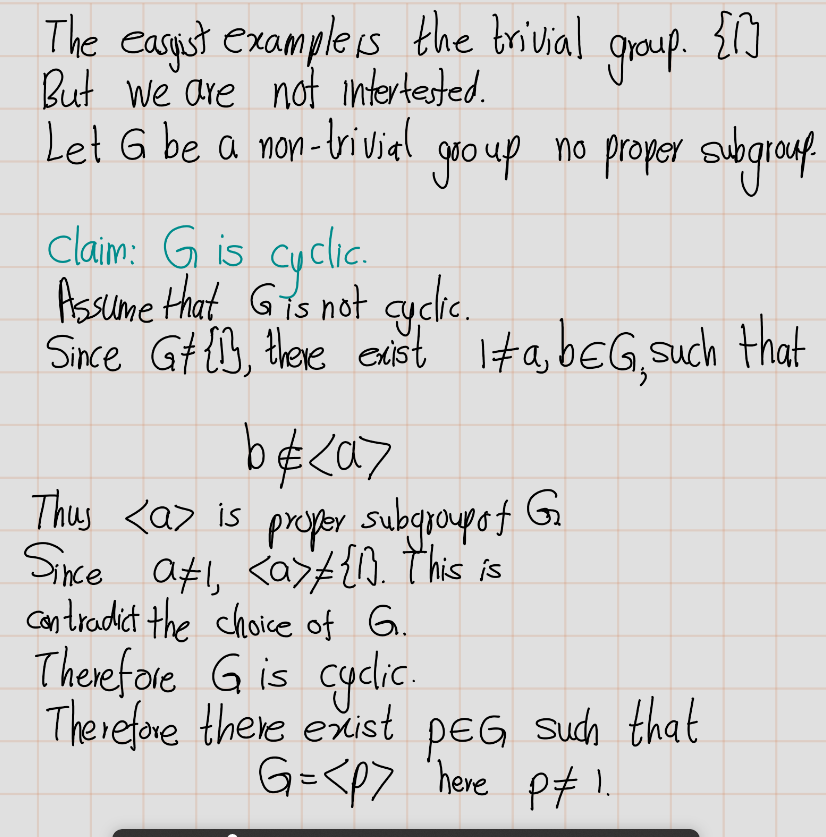
\includegraphics{figures/ch_2/fig54.png}
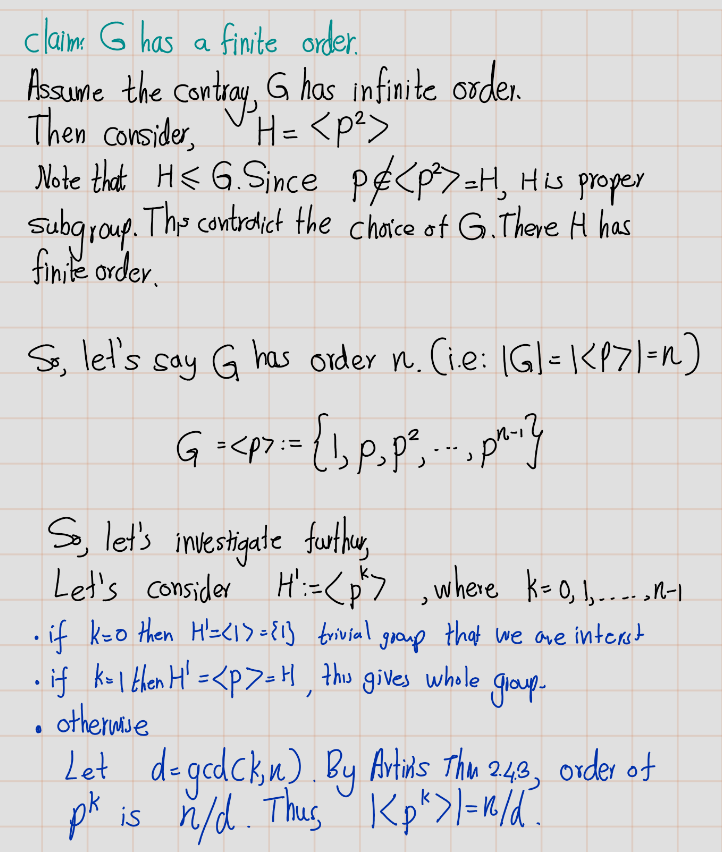
\includegraphics{figures/ch_2/fig55.png}
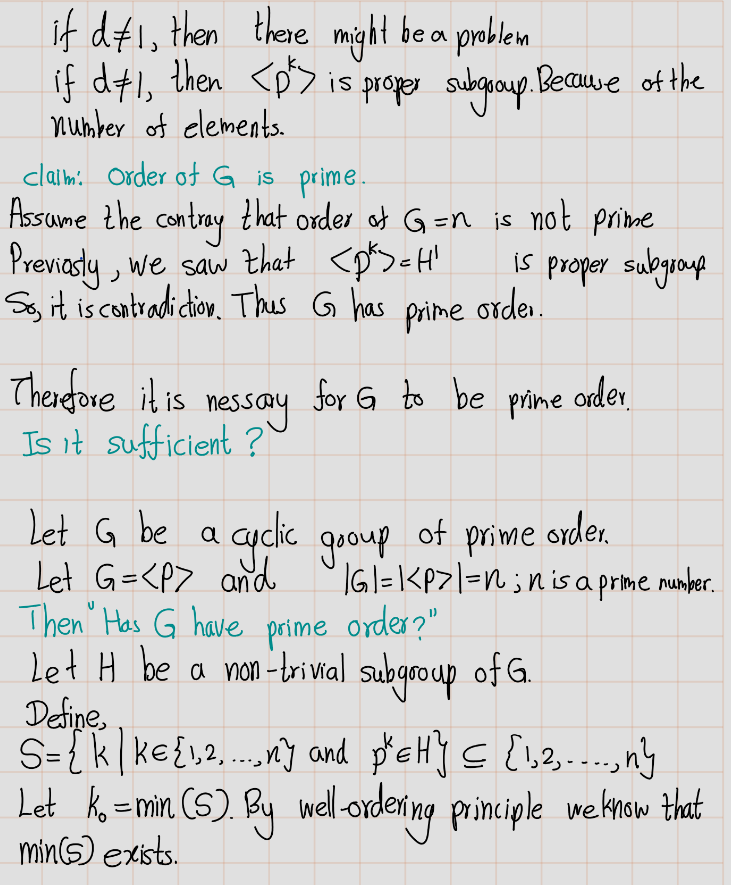
\includegraphics{figures/ch_2/fig56.png}
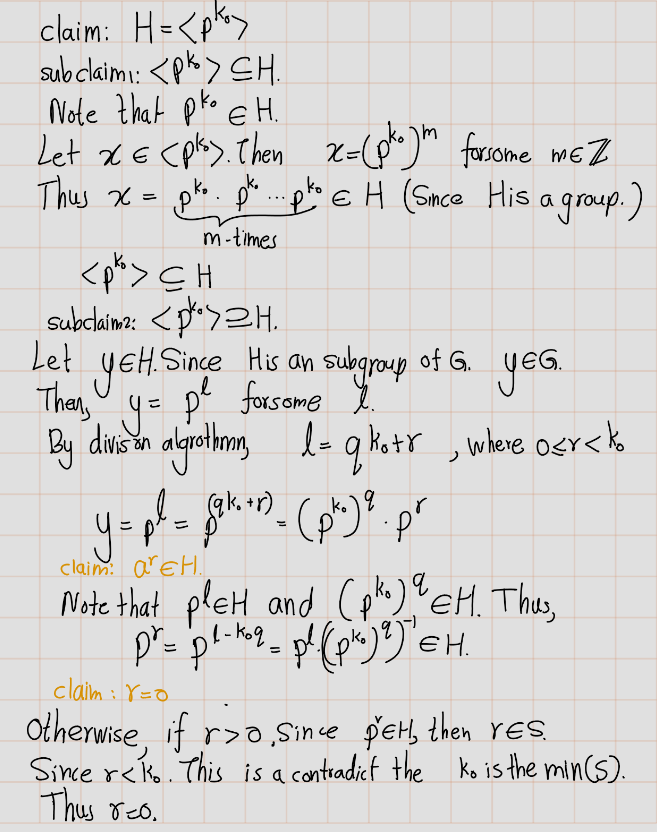
\includegraphics{figures/ch_2/fig57.png}
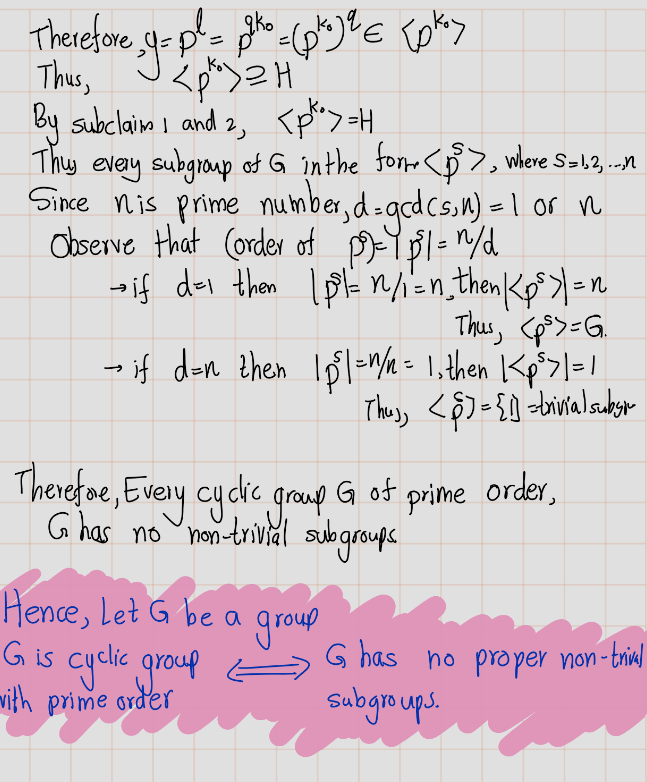
\includegraphics{figures/ch_2/fig58.png}

\begin{exercise}[Artin 2.4.5]
\protect\hypertarget{exr:unnamed-chunk-94}{}\label{exr:unnamed-chunk-94}Prove that every subgroup of a cyclic group is cyclic. Do this by working with exponents, and use the description of the subgroups of \((\mathbb{Z},+)\).
\end{exercise}

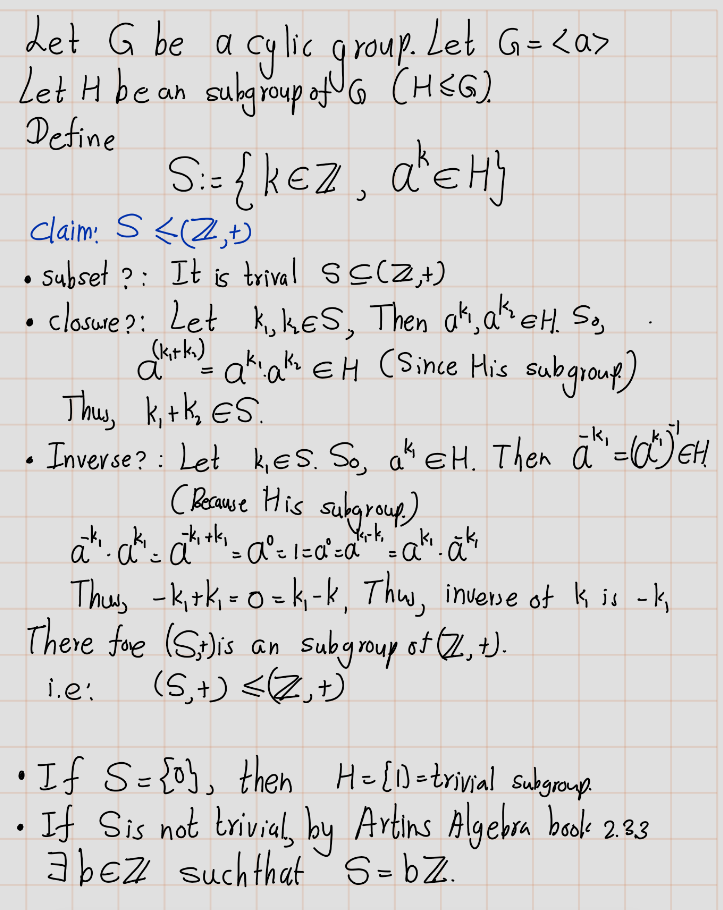
\includegraphics{figures/ch_2/fig59.png}
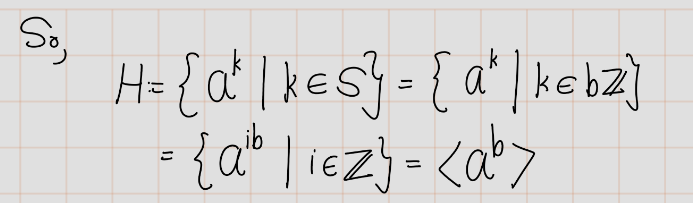
\includegraphics{figures/ch_2/fig60.png}

\begin{exercise}[Artin 2.4.6]
\protect\hypertarget{exr:unnamed-chunk-97}{}\label{exr:unnamed-chunk-97}\leavevmode

\begin{enumerate}
\def\labelenumi{(\alph{enumi})}
\tightlist
\item
  Let \(G\) be a cyclic group of order 6. How many of its elements generate \(G\)?\\
  Answer the same question for cyclic groups of orders 5 and 8.
\item
  Describe the number of elements that generate a cyclic group of arbitrary order \(n\).
\end{enumerate}

\end{exercise}

\textbf{Solution}:

\begin{enumerate}
\def\labelenumi{\alph{enumi})}
\tightlist
\item
\end{enumerate}

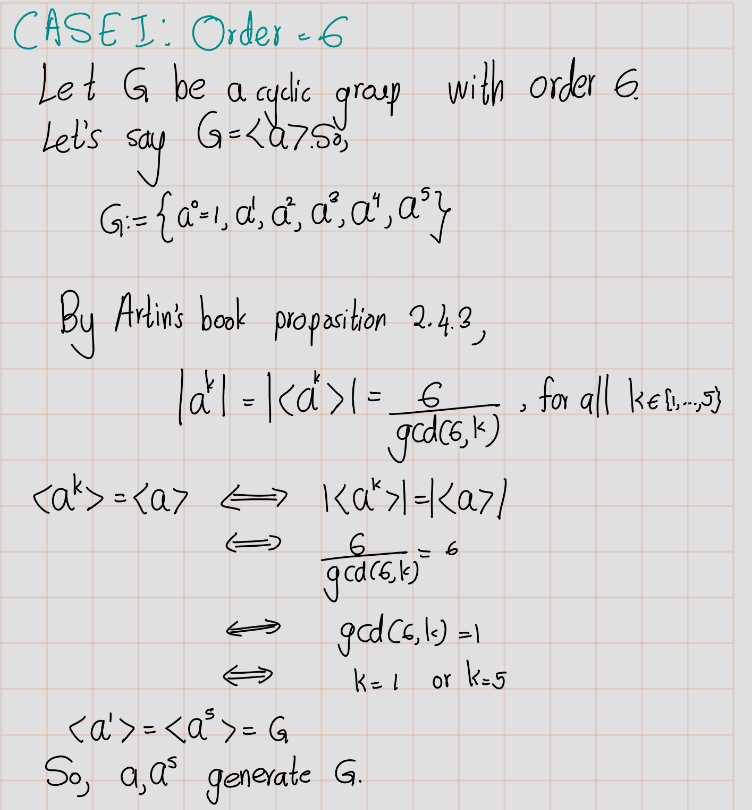
\includegraphics{figures/ch_2/fig61.png}
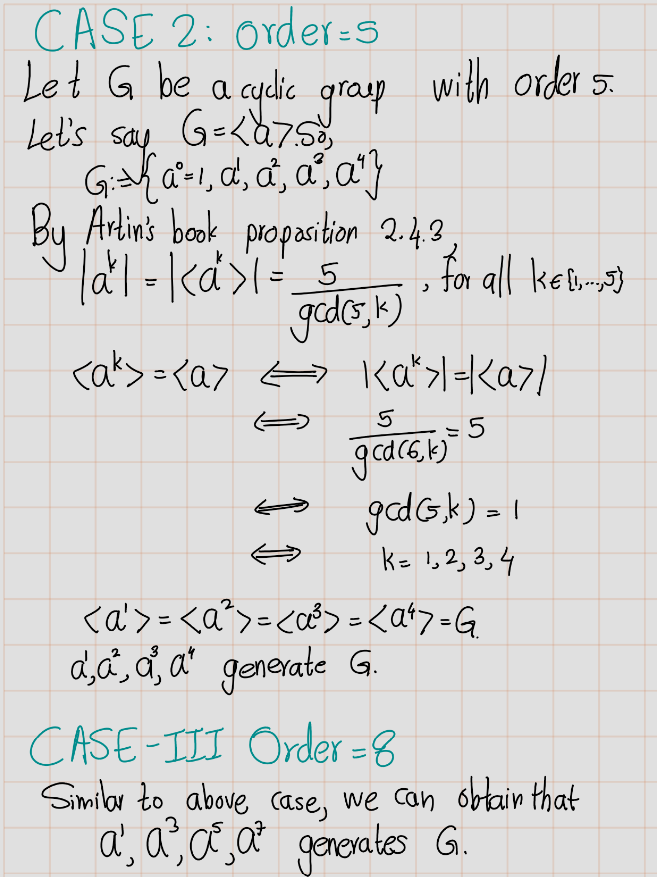
\includegraphics{figures/ch_2/fig62.png}
b)
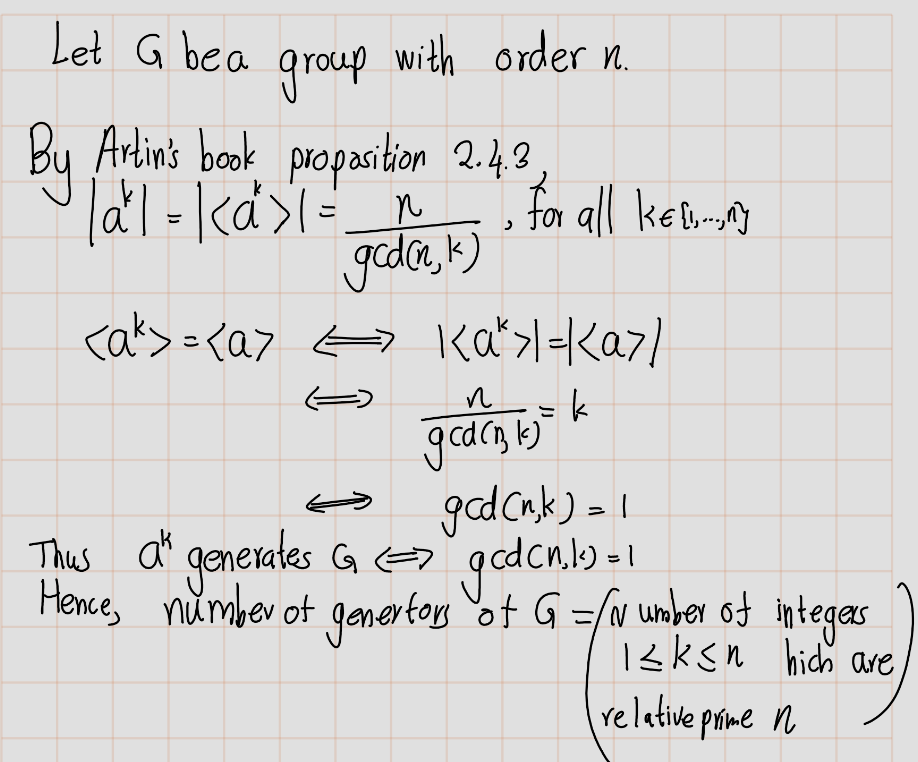
\includegraphics{figures/ch_2/fig63.png}

\begin{exercise}[Artin 2.4.7]
\protect\hypertarget{exr:unnamed-chunk-101}{}\label{exr:unnamed-chunk-101}Let \(x\) and \(y\) be elements of a group \(G\). Assume that each of the elements \(x\), \(y\), and \(xy\) has order 2. Prove that the set \(H = \{I, x, y, xy\}\) is a subgroup of \(G\), and that it has order 4.
\end{exercise}

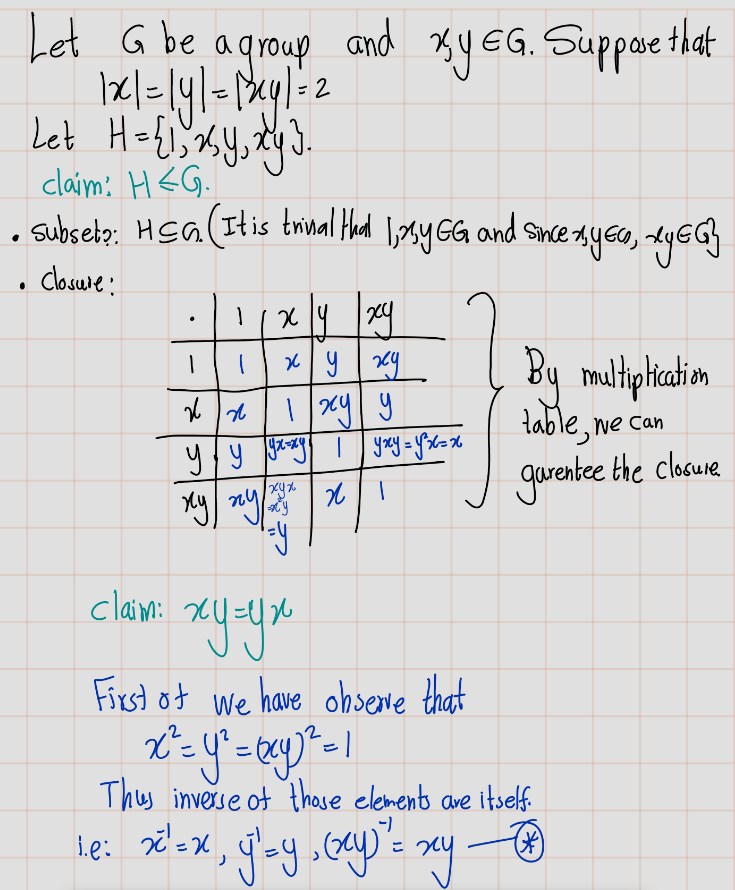
\includegraphics{figures/ch_2/fig64.png}
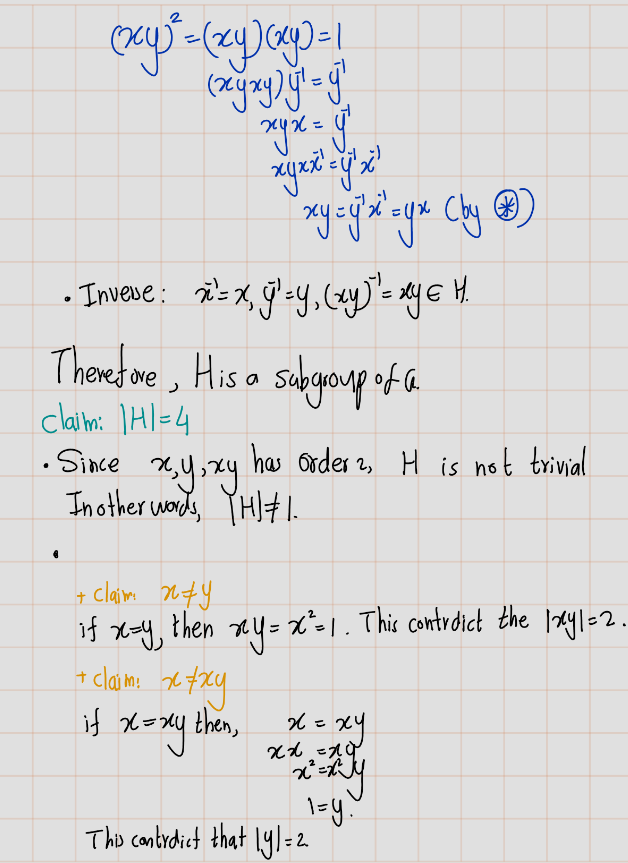
\includegraphics{figures/ch_2/fig65.png}
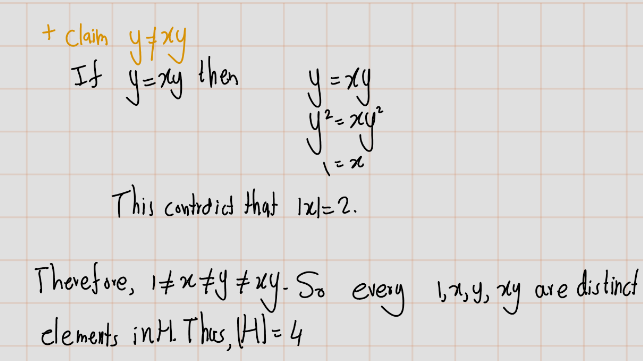
\includegraphics{figures/ch_2/fig66.png}

\begin{exercise}[Artin 2.4.8]
\protect\hypertarget{exr:unnamed-chunk-105}{}\label{exr:unnamed-chunk-105}\leavevmode

\begin{enumerate}
\def\labelenumi{\alph{enumi})}
\tightlist
\item
  Prove that the elementary matrices of the first and third types (1.2.4) generate \(GL_n(\mathbb{R})\).
\item
  Prove that the elementary matrices of the first type generate \(SL_n(K)\). Do the \(2 \times 2\) case first.
\end{enumerate}

\end{exercise}

Recall the types of elementary matrices,

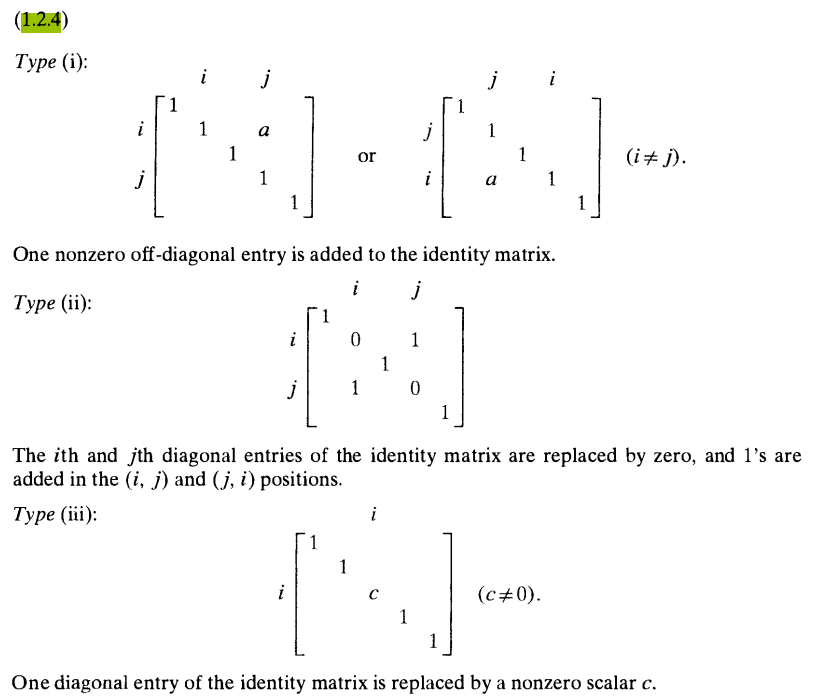
\includegraphics{figures/ch_2/fig67.png}

\begin{exercise}[Artin 2.4.9]
\protect\hypertarget{exr:unnamed-chunk-107}{}\label{exr:unnamed-chunk-107}How many elements of order \(2\) does the symmetric group \(S_4\) contain?
\end{exercise}

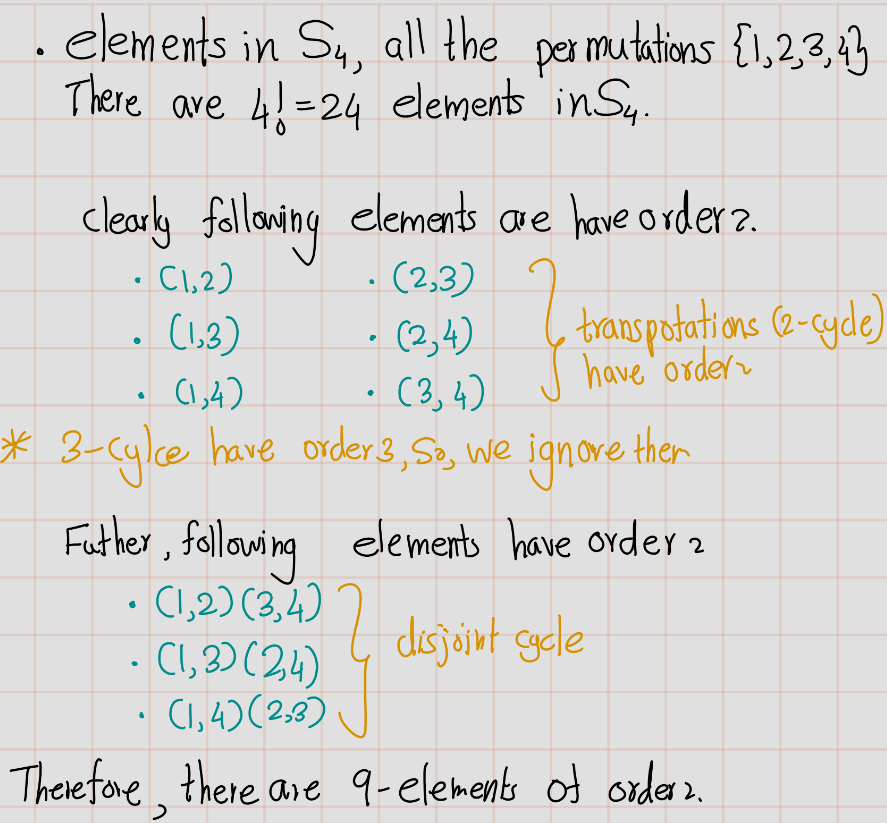
\includegraphics{figures/ch_2/fig68.png}
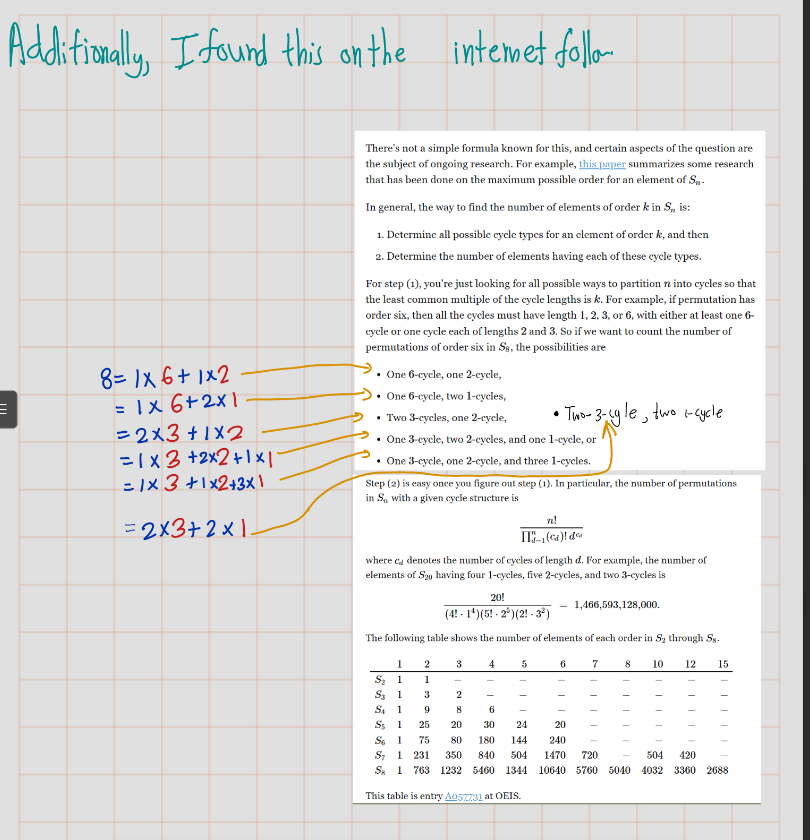
\includegraphics{figures/ch_2/fig69.png}
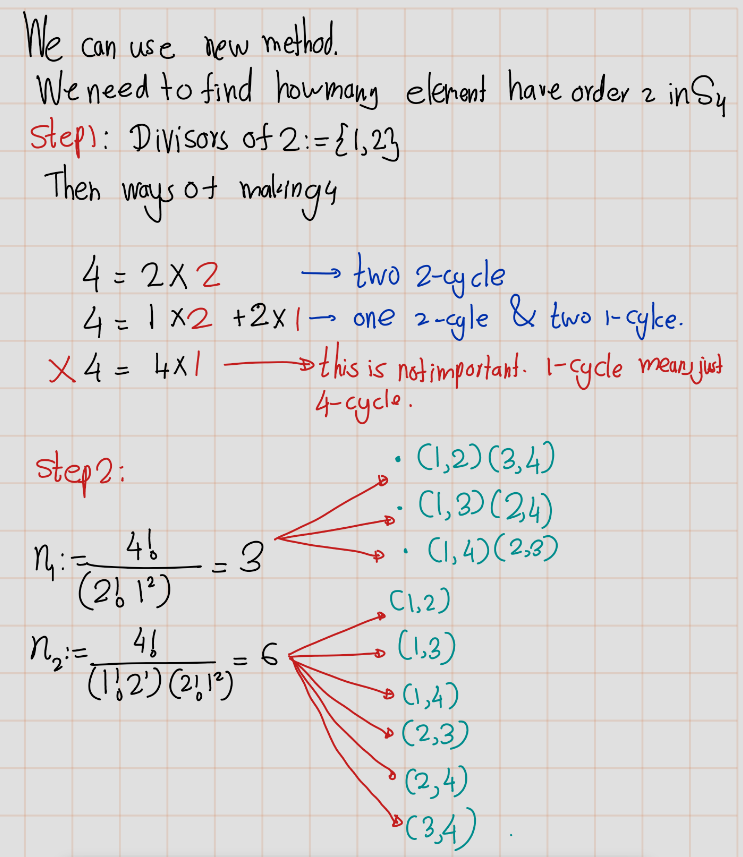
\includegraphics{figures/ch_2/fig70.png}

\begin{exercise}[Artin 2.4.10]
\protect\hypertarget{exr:unnamed-chunk-111}{}\label{exr:unnamed-chunk-111}Show by example that the product of elementsof finite order in a group need not have finite order. What if the group is abelian?
\end{exercise}

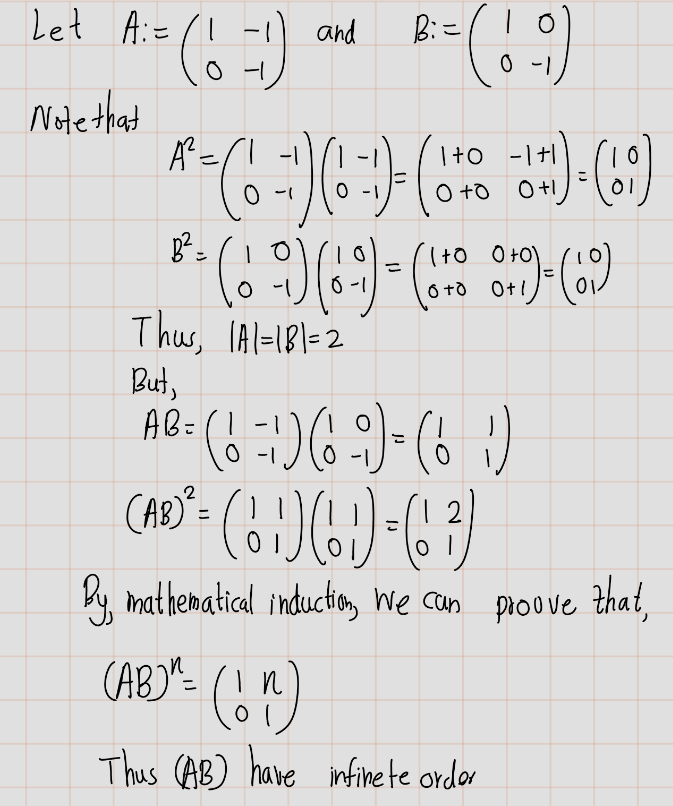
\includegraphics{figures/ch_2/fig71.png}
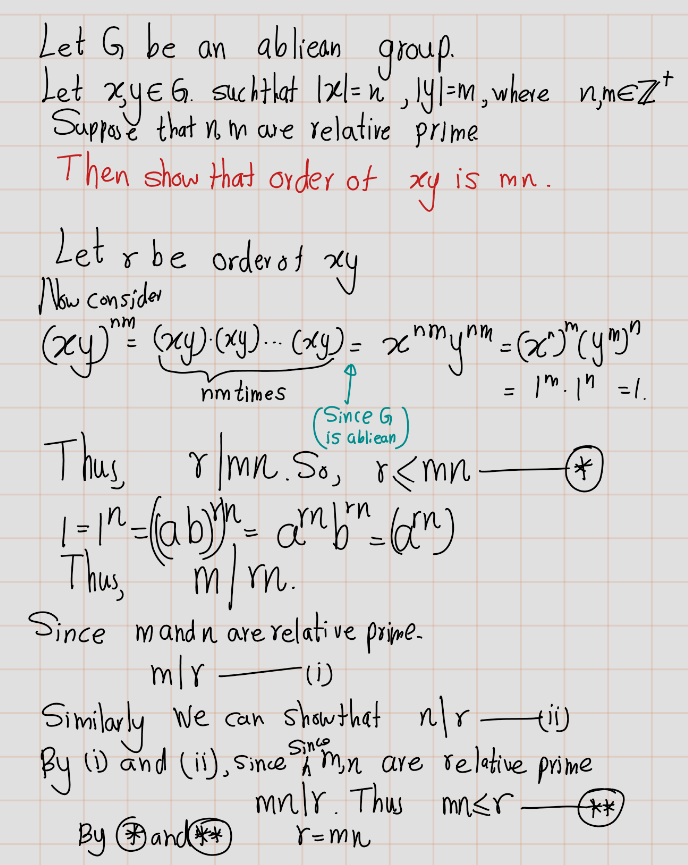
\includegraphics{figures/ch_2/fig72.png}

\hypertarget{homomorphisms-1}{%
\subsection{Homomorphisms}\label{homomorphisms-1}}

\begin{exercise}[Artin 2.5.1]
\protect\hypertarget{exr:unnamed-chunk-114}{}\label{exr:unnamed-chunk-114}Let \(\varphi: G \rightarrow G'\) be a surjective homomorphism. Prove that if \(G\) is cyclic, then \(G'\) is cyclic, and if \(G\) is abelian, then \(G'\) is abelian.
\end{exercise}

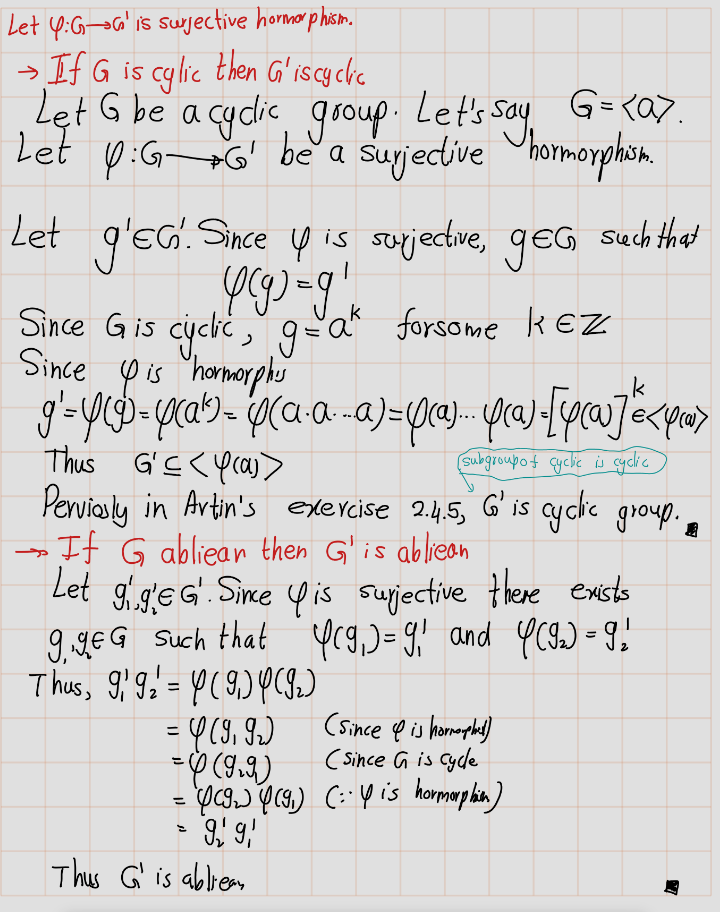
\includegraphics{figures/ch_2/fig73.png}

\begin{exercise}[Artin 2.5.2]
\protect\hypertarget{exr:unnamed-chunk-116}{}\label{exr:unnamed-chunk-116}Prove that the intersection \(K \cap H\) ofsubgroupsof a group \(G\) is a subgroup of \(H\), and that if \(K\) is a normal subgroup of \(G\), then \(K \cap H\) is a normal subgroup of \(H\).
\end{exercise}

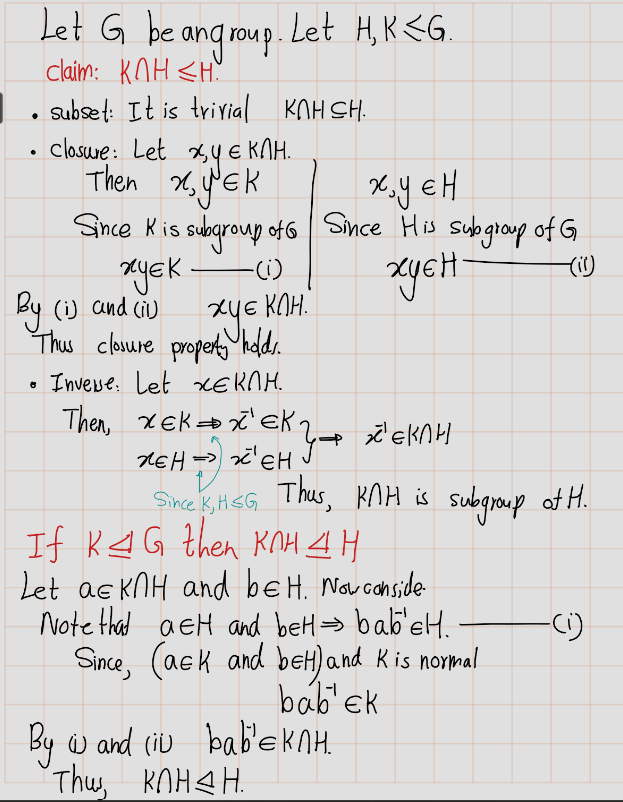
\includegraphics{figures/ch_2/fig74.png}

\begin{exercise}[Artin 2.5.3]
\protect\hypertarget{exr:unnamed-chunk-118}{}\label{exr:unnamed-chunk-118}Let \(U\) denote the group of invertible upper triangular \(2 \times 2\) matrices \(A = \begin{bmatrix} a & b \\ 0 & d \end{bmatrix}\), and let \(\varphi : U \rightarrow \mathbb{R}^{\times}\) be the map that sends \(A\) to \(a^2\). Prove that \(\varphi\) is a homomorphism, and determine its kernel and image.
\end{exercise}

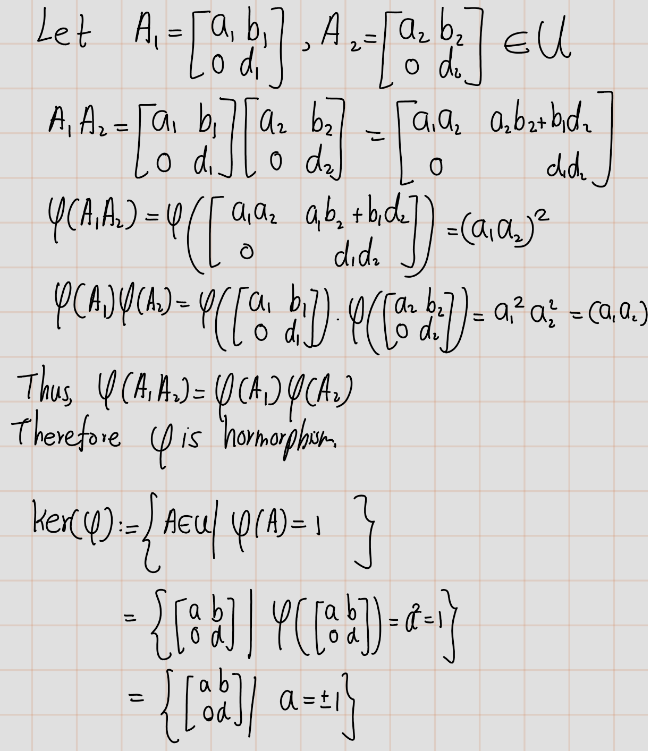
\includegraphics{figures/ch_2/fig75.png}
\includegraphics{figures/ch_2/fig76.png}

\begin{exercise}[Artin 2.5.4]
\protect\hypertarget{exr:unnamed-chunk-121}{}\label{exr:unnamed-chunk-121}Let \(f: (\mathbb{R},+) \rightarrow (\mathbb{C},\times)\) be the map \(f(x) = e^{ix}\). Prove that \(f\) is a homomorphism, and determine its kernel and image.
\end{exercise}

\includegraphics{figures/ch_2/fig77.png}

\begin{exercise}[Artin 2.5.5]
\protect\hypertarget{exr:unnamed-chunk-123}{}\label{exr:unnamed-chunk-123}Prove that the \(n \times n\) matrices that have the block form \(M = \begin{bmatrix} A & B \\ 0 & D \end{bmatrix}\), with \(A \in GL_r(\mathbb{R})\) and \(D \in GL_{n-r}(\mathbb{R})\), form a subgroup \(H\) of \(GL_n(\mathbb{R})\), and that the map \(H \rightarrow GL_r(\mathbb{R})\) that sends \(M \mapsto A\) is a homomorphism. What is its kernel?
\end{exercise}

\begin{exercise}[Artin 2.5.6]
\protect\hypertarget{exr:unnamed-chunk-124}{}\label{exr:unnamed-chunk-124}Determine the center of \(GL_n (\mathbb{R})\).

\emph{Hint:} You are asked to determine the invertible matrices \(A\) that commute with every invertible matrix \(B\). Do not test with a general matrix \(B\). Test with elementary matrices.
\end{exercise}

\hypertarget{isomorphisms-1}{%
\subsection{Isomorphisms}\label{isomorphisms-1}}

\begin{exercise}[Artin 2.6.1]
\protect\hypertarget{exr:unnamed-chunk-125}{}\label{exr:unnamed-chunk-125}Let \(G'\) be the group of real matrices of the form
\(\begin{bmatrix}1 & x \\ & 1\end{bmatrix}\)
Is the map \(\phi: (\mathbb{R},+) \rightarrow G'\) that sends \(x\) to this matrix an isomorphism?
\end{exercise}

\includegraphics{figures/ch_2/fig78.png}

\begin{exercise}[Artin 2.6.2]
\protect\hypertarget{exr:unnamed-chunk-127}{}\label{exr:unnamed-chunk-127}Describe all homomorphisms \(\phi : (\mathbb{Z},+) \rightarrow (\mathbb{Z},+)\). Determine which are injective, which are surjective, and which are isomorphisms.
\end{exercise}

\includegraphics{figures/ch_2/fig79.png}
\includegraphics{figures/ch_2/fig80.png}
\includegraphics{figures/ch_2/fig81.png}

\begin{exercise}[Artin 2.6.3]
\protect\hypertarget{exr:unnamed-chunk-131}{}\label{exr:unnamed-chunk-131}Show that the functions \(f = \frac{1}{x}\), \(g = \frac{x - 1}{x}\) generate a group of functions, the law of composition being composition of functions, that is isomorphic to the symmetric group \(S_3\).
\end{exercise}

\begin{exercise}[Artin 2.6.4]
\protect\hypertarget{exr:unnamed-chunk-132}{}\label{exr:unnamed-chunk-132}Prove that in a group, the products \(ab\) and \(ba\) are conjugate elements.
\end{exercise}

\includegraphics{figures/ch_2/fig82.png}

\begin{exercise}[Artin 2.6.5]
\protect\hypertarget{exr:unnamed-chunk-134}{}\label{exr:unnamed-chunk-134}Decide whether or not the two matrices \(A = \begin{bmatrix} 3 & 0 \\ 0 & 2 \end{bmatrix}\) and \(B = \begin{bmatrix} 1 & 1 \\ -2 & 4 \end{bmatrix}\) are conjugate elements of the general linear group \(GL_2(\mathbb{R})\).
\end{exercise}

\includegraphics{figures/ch_2/fig83.png}

\includegraphics{figures/ch_2/fig84.png}

\includegraphics{figures/ch_2/fig85.png}

\includegraphics{figures/ch_2/fig86.png}

\begin{exercise}[Artin 2.6.7]
\protect\hypertarget{exr:unnamed-chunk-139}{}\label{exr:unnamed-chunk-139}Let \(H\) be a subgroup of \(G\), and let \(g\) be a fixed element of \(G\). The conjugate subgroup \(gHg^{-1}\) is defined to be the set of all conjugates \(ghg^{-1}\), with \(h\) in \(H\). Prove that \(gHg^{-1}\) is a subgroup of \(G\).
\end{exercise}

\includegraphics{figures/ch_2/fig87.png}

\begin{exercise}[Artin 2.6.8]
\protect\hypertarget{exr:unnamed-chunk-141}{}\label{exr:unnamed-chunk-141}Prove that the map \(A \mapsto (A^{t})^{-1}\) is an automorphism of \(GL_{n}(\mathbb{R})\).
\end{exercise}

\includegraphics{figures/ch_2/fig88.png}

\begin{exercise}[Artin 2.6.9]
\protect\hypertarget{exr:unnamed-chunk-143}{}\label{exr:unnamed-chunk-143}Prove that a group \(G\) and its opposite group \(G^{o}\) (Exercise 2.2.6) are isomorphic.
\end{exercise}

\includegraphics{figures/ch_2/fig89.png}

\begin{exercise}[Artin 2.6.10]
\protect\hypertarget{exr:unnamed-chunk-145}{}\label{exr:unnamed-chunk-145}

Find all automorphisms of

\begin{enumerate}
\def\labelenumi{(\alph{enumi})}
\tightlist
\item
  a cyclic group of order 10,
\item
  the symmetric group \(S_{3}\).
\end{enumerate}

\end{exercise}

\includegraphics{figures/ch_2/fig90.png}

\begin{exercise}[Artin 2.6.11]
\protect\hypertarget{exr:unnamed-chunk-147}{}\label{exr:unnamed-chunk-147}Let \(a\) be an element of a group \(G\). Prove that if the set \(\{1, a\}\) is a normal subgroup of \(G\), then \(a\) is in the center of \(G\).
\end{exercise}

\includegraphics{figures/ch_2/fig91.png}

\hypertarget{equivalence-relations-and-partitions-1}{%
\subsection{Equivalence Relations and Partitions}\label{equivalence-relations-and-partitions-1}}

\hypertarget{cosets-1}{%
\subsection{Cosets}\label{cosets-1}}

\hypertarget{modular-arthmetic}{%
\subsection{Modular Arthmetic}\label{modular-arthmetic}}

\begin{exercise}
\protect\hypertarget{exr:unnamed-chunk-149}{}\label{exr:unnamed-chunk-149}What are the possible values of \(a^2\) modulo 4? modulo 8?
\end{exercise}

\textbf{solution}:

\begin{itemize}
\item
  \emph{In modulo 4}\\
  \begin{eqnarray*}
    \overline{0}^2&\equiv & 0 \pmod{4}\\
    \overline{1}^2&\equiv & 1 \pmod{4}\\
    \overline{2}^2&\equiv & 0 \pmod{4}\\
    \overline{3}^2&\equiv & 1 \pmod{4}\\
  \end{eqnarray*}
  The possible values of \(a^2\pmod{4}\) are 0 and 1.
\item
  \emph{In modulo 8}\\
  \begin{eqnarray*}
    \overline{0}^2&\equiv & 0 \pmod{8}\\
    \overline{1}^2&\equiv & 1 \pmod{8}\\
    \overline{2}^2&\equiv & 4 \pmod{8}\\
    \overline{3}^2&\equiv & 1 \pmod{8}\\
    \overline{4}^2&\equiv & 0 \pmod{8}\\
    \overline{5}^2&\equiv & 1 \pmod{8}\\
    \overline{6}^2&\equiv & 4 \pmod{8}\\
    \overline{7}^2&\equiv & 1 \pmod{8}\\
  \end{eqnarray*}
  The possible values of \(a^2\pmod{8}\) are 0,1 and 4.
\end{itemize}

\begin{exercise}
\protect\hypertarget{exr:unnamed-chunk-150}{}\label{exr:unnamed-chunk-150}Prove that every integer \(a\) is congruent to the sum of its decimal digits modulo 9.
\end{exercise}

\begin{proof}
Let \(x\in \mathbb{Z}\). Now we can represent \(x\) as follows

\[x=a_010^0+a_110^1+\cdots +a_n10^n=\sum_{i=0}^n a_{i}10^i\text{  forsome } n\in \mathbb{Z},\text{ and }a_i\in \{0,1,...,9\}\]

We need to show \(x \equiv \sum_{i=0}^na_i\pmod{9}\). So, now consider,

\begin{eqnarray}
x-\sum_{i=0}^n a_{i}&=&\sum_{i=0}^n a_{i}10^i-\sum_{i=0}^n a_{i}\\
&=& \sum_{i=0}^n (a_{i}10^i- a_{i})\\
&=& \sum_{i=0}^n a_{i}(10^i- 1)
\end{eqnarray}

By follwing calim we can get that,

\begin{eqnarray}
x-\sum_{i=0}^n a_i &\equiv & 0 \pmod{9}\\
x &\equiv & \sum_{i=0}^na_i\pmod{9}
\end{eqnarray}
\end{proof}

\textbf{Claim}: \(9|(10^k-1)\) for any \(k\in \mathbb{N}\).

\begin{proof}
We use mathematical induction.\\
\emph{\(k=1\)}\\
This case is trivial. Because \(9|10-1\).\\
\emph{\(k=n\in\mathbb{Z}\)}\\
Now asuume when \(n=k, 9|(10^n-1)\).\\
\emph{\(k=n+1\)}
\[10^{n+1}-1 =10\cdot 10^{n}-1=9\cdot 10^n + (10^n - 1) \]
Thus \(9\vert (10^{n+1}-1)\).\\
Therefore,by mathematical induction, \(9|(10^n-1)\) for any \(n\in \mathbb{N}\).
\end{proof}

\begin{exercise}
\protect\hypertarget{exr:unnamed-chunk-153}{}\label{exr:unnamed-chunk-153}Solve the congruence \(2x \equiv 5\) modulo 9 and modulo 6.
\end{exercise}

Done Later add.

\begin{exercise}
\protect\hypertarget{exr:unnamed-chunk-154}{}\label{exr:unnamed-chunk-154}Determine the integers \(n\) for which the pair of congruences \(2x - y \equiv 1\) and \(4x + 3y \equiv 2\) modulo \(n\) has a solution.
\end{exercise}

Done Later add.

\begin{exercise}
\protect\hypertarget{exr:unnamed-chunk-155}{}\label{exr:unnamed-chunk-155}Prove the Chinese Remainder Theorem: Let \(a, b, u, v\) be integers, and assume that the greatest common divisor of \(a\) and \(b\) is 1. Then there is an integer \(x\) such that \(x \equiv u\) modulo \(a\) and \(X \equiv v\) modulo \(b\).\\
Hint: Do the case \(u = 0\) and \(v = 1\) first.
\end{exercise}

\begin{exercise}
\protect\hypertarget{exr:unnamed-chunk-156}{}\label{exr:unnamed-chunk-156}Determine the order of each of the matrices A and B when the matrix entries are interpreted modulo 3.
\end{exercise}

\hypertarget{product-group}{%
\subsection{Product Group}\label{product-group}}

\begin{exercise}
\protect\hypertarget{exr:unnamed-chunk-157}{}\label{exr:unnamed-chunk-157}Let \(x\) be an element of order \(r\) of a group \(G\), and let \(y\) be an element of \(G'\) of order \(s\). What is the order of \((x, y)\) in the product group \(G \times G'\)?
\end{exercise}

\textbf{Solution}: The order of \((x, y)\) in the product group \(G \times G'\) is \(lcm(r,s)\)\\
Let \(n\in \mathbb{Z}^+\) such that \[(x,y)^n=(x^n,y^n)=(1_G,1_{G'}).\]
This implies, \(x^n=1_G\) and \(y^n=1_{G'}\). Since order of \(x\) and \(y\) are \(r\) and \(s\) respectively,
\[r|n~~~\text{ and }~~~s|n\]
So, we know that the least positive integer such that above property holds is \(lcm(r,s)\). Hence,The order of \((x, y)\) in the product group \(G \times G'\) is \(lcm(r,s)\).

\begin{exercise}
\protect\hypertarget{exr:unnamed-chunk-158}{}\label{exr:unnamed-chunk-158}What does Proposition \ref{prp:prp2114} tell us when, with the usual notation for the symmetric
group \(S_3,K\) and \(H\) are the subgroups \(<y>\) and \(<x>\)?
\end{exercise}

Recall: \(y^2=1\) and \(x^3=1\). Then
\[H=<x>=\{1,x,x^2\}~~~\text{ and }~~~ K=<y>=\{1,y\}\]
Let the multiplication map, \(f:H\times K \to S_3\) defined by \(f(h,k)=hk\). Then,
\(Im(f)=HK=\{hk:h\in <x>, k\in <y>\}=\{1,x,x^2,y,xy,x^2y\}\).

\textbf{Claim 1}: \(f\) is injective.\\
Observe that \(H \cap K=\{1\}\). by \ref{prp:prp2114} a) \(f\) is injective.

\textbf{Claim 2}: \(f\) is surjective.\\
Observe that \(S_3=HK=\{1,x,x^2,y,xy,x^2y\}\). Thus, \(f\) is surjective.

\textbf{Claim 3} : \(f\) is not homomorphism.\\
\begin{eqnarray}
f((x,y)\cdot (x,1))&=& f(x^2,y^2)=f(x^2,1)=x^2\cdot 1=x^2\\
f(x,y)\cdot f(x,1)&=& (x\cdot y)\cdot (x\cdot 1)=(xy)\cdot x=y
\end{eqnarray}
Thus, \(f\) is not a homomorphism.

\begin{exercise}
\protect\hypertarget{exr:unnamed-chunk-159}{}\label{exr:unnamed-chunk-159}Prove that the product of two infinite cyclic groups is not infinite cyclic.
\end{exercise}

\begin{proof}
\leavevmode

\begin{itemize}
\item
  \textbf{Claim 1} : Infinite cyclic groups are isomorphic to \(Z\).\\
  Let \(G\) be a infinte cyclic group and \(<a>=G\).
  We can define a function \(f: \mathbb{Z} \rightarrow G\) by \(f(n) = a^n\) for all integers \(n\). We need to show that \(f\) is an isomorphism, which means it is bijective.

  \begin{itemize}
  \tightlist
  \item
    \textbf{Subclaim 1.1} : \(f\) is a hormorphism.\\
    \[f(n+m)=a^{n+m}=a^n \cdot a^m =f(n)\cdot f(m)\]
    Thus, \(f\) is a hormorphism.
  \item
    \textbf{Subclaim 1.2} :\(f\) is a injective\\
    Suppose that \(f(n)=f(m)\)
    \begin{eqnarray}
      f(n)&=&f(m)\\
      a^n &=& a^m \\
      n&=& m ~~(\text{Since order is infinite})
    \end{eqnarray}
  \item
    \textbf{Subclaim 1.3} : \(f\) is surjective.\\
    Let \(x\in G=<a>\). Then, \(x=a^k\) for some \(k\in \mathbb{Z}\). Then, observe that
    \[f(k)=a^k=a \].
    Thus, \(f\) is surjective.
  \end{itemize}
\end{itemize}

Therefore, \(f\) is an isomorphism. Thus, the infinite cyclic groups are isomorphic to \(\mathbb{Z}\).

We can consider \(\mathbb{Z}\times \mathbb{Z}\). Suppose that \((a, b)\) generate the product group. But then, we see that \((2a, b)\) cannot be obtained from adding \((a, b)\) to itself, which implies that \(\mathbb{Z}\times \mathbb{Z}\) is not infinite cyclic.

\end{proof}

\begin{exercise}
\protect\hypertarget{exr:unnamed-chunk-161}{}\label{exr:unnamed-chunk-161}

In each of the following cases, determine whether or not \(G\) is isomorphic to the product group \(H \times K\).

\begin{enumerate}
\def\labelenumi{(\alph{enumi})}
\item
  \(G = \mathbb{R}^\times\), \(H = \{\pm 1\}\), \(K = \{\)positive real numbers\(\}\).
\item
  \(G = \{\)invertible upper triangular \(2 \times 2\) matrices\(\}\), \(H = \{\)invertible diagonal matrices\(\}\), \(K = \{\)upper triangular matrices with diagonal entries \(1\}\).
\item
  \(G = e^x\), \(H = \{\)unit circle\(\}\), \(K = \{\)positive real numbers\(\}\).
\end{enumerate}

\end{exercise}

\textbf{Solution}:

\begin{enumerate}
\def\labelenumi{(\alph{enumi})}
\item
  Observe that \(G=\mathbb{R}^\times=\mathbb{R}\setminus\{0\}\) is abelian. Then \(H,K \trianglelefteq G\). Further, observe that \(H\cap K=\{1\}\) and \(HK=\mathbb{R}^\times=G\). Thus, by proposition \ref{prp:prp2114} \(G \cong H \times K\).
\item
\end{enumerate}

\begin{itemize}
\item
  \textbf{Claim b.1}: \(K\trianglelefteq G\).\\
  Let \(g = \begin{bmatrix} a & b \\ & c \end{bmatrix}\) be an arbitary matrix in \(G\) and \(k = \begin{bmatrix} 1 & d \\ & 1 \end{bmatrix}\in K\).
  Then,
  \[ g^{-1} = \begin{bmatrix}
  a^{-1} & -ba^{-1}c^{-1} \\
  & c^{-1}
  \end{bmatrix}\]
  Then
  \[gkg^{-1} = \begin{bmatrix}
  a & b \\
  & c
  \end{bmatrix}\begin{bmatrix}
  1 & d \\
  & 1
  \end{bmatrix}\begin{bmatrix}
  a^{-1} & -ba^{-1}c^{-1} \\
  & c^{-1}
  \end{bmatrix}\]
  \[= \begin{bmatrix}
  a & b \\
  & c
  \end{bmatrix}\begin{bmatrix}
  a^{-1} & dc^{-1} - ba^{-1}c^{-1} \\
  & c^{-1}
  \end{bmatrix} = \begin{bmatrix}
  1 & adc^{-1} \\
  & 1
  \end{bmatrix} \in K\]
  Thus, \(H\trianglelefteq G\).
\item
  \textbf{Claim b.2} : \(H=Z(G)\) (\(H\) is in the center of \(G\)).

  \begin{itemize}
  \tightlist
  \item
    \emph{subclaim b.2.1} : \(H \subseteq Z(G)\).\\
    Let \(h=\begin{bmatrix} x & 0 \\ & x \end{bmatrix} \in H\). Then,
    \[B=\begin{bmatrix}
    x & 0 \\
    & x
    \end{bmatrix}=x\begin{bmatrix}
    1 &  \\
    & 1
    \end{bmatrix}=BI\]
    Then observe that, for any \(A\in G\),
    \[BA=(xI)A = xA = Ax = A(xI)=AB\]
  \item
    \emph{subclaim b.2.2} : \(H \supseteq Z(G)\).\\
    Let \(\begin{bmatrix} p & q \\ r & s \end{bmatrix}\in Z(G)\), then,
  \end{itemize}
\end{itemize}

\begin{eqnarray}
\begin{bmatrix}
p & q \\
r & s
\end{bmatrix}\begin{bmatrix}
1 & 0 \\
0 & -1
\end{bmatrix} &=& \begin{bmatrix}
1 & 0 \\
0 & -1
\end{bmatrix}\begin{bmatrix}
p & q \\
r & s
\end{bmatrix}\\
\begin{bmatrix}
p & -q \\
r & -s
\end{bmatrix}&=& \begin{bmatrix}
p & q \\
-r & -s
\end{bmatrix}\\
\end{eqnarray}
This yields \(-q = q\) and \(r = -r\) which imply \(q = r = 0\). Now considering,

\begin{eqnarray}
\begin{bmatrix}
p & 0 \\
0 & s
\end{bmatrix}\begin{bmatrix}
0 & 1 \\
1 & 0
\end{bmatrix} &=& \begin{bmatrix}
0 & 1 \\
1 & 0
\end{bmatrix}\begin{bmatrix}
p & 0 \\
0 & s
\end{bmatrix}\\
\begin{bmatrix}
0 & p \\
q & 0
\end{bmatrix}&=& \begin{bmatrix}
0 & q \\
p & 0
\end{bmatrix}\\
\end{eqnarray}
This implies that \(a = d\) and since the matrix is invertible, \(a\neq 0\). Thus, \(H \supseteq Z(G)\).

Therefore, \(H = Z(G)\). In other words, \(H\) is in the center of \(G\).

\begin{itemize}
\item
  \textbf{Claim b.2} : \(H\trianglelefteq G\).\\
  Since, \(H\) is in the center of \(G\), then \(H\) is normal.
\item
  \textbf{Claim b.3} : \(H\cap K=\{I\}\).\\
  This is trivial.
\item
  \textbf{Claim b.4} : \(HK=G\)
  Clearly, \(HK\subseteq G\). Conversly,
  for any \(g\in G\), \(a\neq 0, b\neq 0\),
  \[g=\begin{bmatrix}
  a & b \\
  & c
  \end{bmatrix}=\begin{bmatrix}
  a &  \\
  & c
  \end{bmatrix}\begin{bmatrix}
  1 & a^{-1}b \\
  & 1
  \end{bmatrix}\in HK\].
  Thus, \(HK=G\).
\end{itemize}

Therefore, by proposition \ref{prp:prp2114} \(G\cong HK\)

\begin{enumerate}
\def\labelenumi{(\alph{enumi})}
\setcounter{enumi}{2}
\tightlist
\item
  Since \(C^\times\) is abelian, then \(H\) and \(K\) are normal. And, \(H \cap K = \left\lbrace 1 \right\rbrace\).
\end{enumerate}

\includegraphics{figures/ch_2/fig03.png}

Consider \(a + bi \in C^\times\). Then
\[a + bi = \left(\frac{a}{\sqrt{a^2+b^2}} + \frac{b}{\sqrt{a^2+b^2}}i\right)\sqrt{a^2+b^2} \in HK\]
So, \(HK = G\). So, by proposition \ref{prp:prp2114} \(G \cong H \times K\).

\begin{exercise}
\protect\hypertarget{exr:unnamed-chunk-162}{}\label{exr:unnamed-chunk-162}Let \(G_1\) and \(G_2\) be groups, and let \(Z_i\) be the center of \(G_i\). Prove that the center of the product group \(G_1 \times G_2\) is \(Z_1 \times Z_2\).
\end{exercise}

\includegraphics{figures/ch_2/fig04.jpg}

\includegraphics{figures/ch_2/fig05.jpg}

\begin{exercise}
\protect\hypertarget{exr:unnamed-chunk-163}{}\label{exr:unnamed-chunk-163}Let \(G\) be a group that contains normal subgroups of orders \(3\) and \(5\), respectively. Prove that \(G\) contains an element of order \(15\).
\end{exercise}

\begin{exercise}
\protect\hypertarget{exr:unnamed-chunk-164}{}\label{exr:unnamed-chunk-164}Let \(H\) be a subgroup of a group \(G\), let \(\phi:G \to H\) be a homomorphism whose restriction to \(H\) is the identity map, and let \(N\) be its kernel. What can one say about the product map \(H \times N \to G\)?
\end{exercise}

\includegraphics{figures/ch_2/fig06.png}
\includegraphics{figures/ch_2/fig07.jpg}
\includegraphics{figures/ch_2/fig09.png}
\includegraphics{figures/ch_2/fig08.jpg}

\begin{exercise}
\protect\hypertarget{exr:unnamed-chunk-165}{}\label{exr:unnamed-chunk-165}Let \(G\), \(G'\), and \(H\) be groups. Establish a bijective correspondence between homomorphisms \(\phi : H \to G \times G'\) from \(H\) to the product group and pairs \((\varphi, \varphi')\) consisting of a homomorphism \(\varphi:H \to G\) and a homomorphism \(\varphi':H \to G'\).
\end{exercise}

\includegraphics{figures/ch_2/fig10.png}

\includegraphics{figures/ch_2/fig11.jpg}
\includegraphics{figures/ch_2/fig12.jpg}
\includegraphics{figures/ch_2/fig13.jpg}
\includegraphics{figures/ch_2/fig14.jpg}
\includegraphics{figures/ch_2/fig15.jpg}
\includegraphics{figures/ch_2/fig16.jpg}

\begin{exercise}
\protect\hypertarget{exr:unnamed-chunk-166}{}\label{exr:unnamed-chunk-166}Let \(H\) and \(K\) be subgroups of a group \(G\). Prove that the product set \(HK\) is a subgroup of \(G\) if and only if \(HK = KH\).
\end{exercise}

\textbf{Solution} :

\begin{proof}
Let \(G\) be group and \(H,K\leq G\).

\begin{itemize}
\item
  \((\Longrightarrow)\): \textbf{Claim }: if \(HK\leq G\) then \(HK=KH\).\\

  Suppose \(HK\leq G\).

  \begin{itemize}
  \tightlist
  \item
    \textbf{sub claim}:
    Let \(x\in KH\). Then \(x=kh\) for some \(h\in H\) and \(k\in K\),
    \[x=kh=1kh1=(1k)(h1)\in HK\]
    (Since \(1\in H\) and \(1\in K\)). Thus, \(KH \subseteq HK\).\\
  \item
    \textbf{sub claim}: \(KH \supseteq HK\).\\
    We can not use previous method.Because we still do not know \(KH\) is sub group or not.\\
    Let \(y\in HK\). Since \(HK\leq G\), \(y^{-1}\in HK\). Then \(y^{-1}=hk\) for some \(h_0\in H\) and \(k_0\in K\). \textbackslash{}
    \[y=(y^{-1})^{-1}=(h_0k_0)^{-1}=k_0h_0\in KH\]
    Thus, \(KH \supseteq HK\).
  \end{itemize}
\end{itemize}

Therefore, \(KH=HK\).

\begin{itemize}
\tightlist
\item
  \((\Longleftarrow)\): \textbf{Claim }: If \(HK=KH\) then \(HK\leq G\).\\
\end{itemize}

Now suppose that \(HK=KH\).Suppose that \(HK=KH\) is empty. Then, \(H,K\) is empty. Now we use sub group test.\\
- \emph{Closure}: Let \(x,y\in HK\). Then \(x=h_1k_1\) and \(y=h_2k_2\) for some \(h_1,h_2\in H\) and \(k_1,k_2\in K\).
\begin{eqnarray}
  xy&=&(h_1k_1)(h_2k_2)\\
  &=& h_1(k_1h_2)k_2) ~~(\text{By associavity property})\\
  &=& h_1(h_3k_3)k_2) ~\text{for some  }h_3\in H \text{ and } k_3\in K ~(\text{Since} KH=HK)\\
  &=& (h_1h_3)(k_3k_2)\in HK
\end{eqnarray}
- \emph{Inverse}: Let Let \(x\in HK\). Then \(x=h'k'\) for some \(h'\in H\) and \(k'\in K\).
\[x^{-1}=(h'k')^{-1}=k'h'\in KH=HK\]
Thus, \(HK\leq G\).

Therefore, the product set \(HK\) is a subgroup of \(G\) if and only if \(HK = KH\)
\end{proof}

\hypertarget{quotient-groups-1}{%
\subsection{Quotient Groups}\label{quotient-groups-1}}

\begin{exercise}
\protect\hypertarget{exr:unnamed-chunk-168}{}\label{exr:unnamed-chunk-168}Show that if a subgroup \(H\) of a group \(G\) is not normal, there are left cosets \(aH\) and \(bH\)
whose product is not a coset.
\end{exercise}

\begin{proof}
Suppose that \(H \leq G\) but \(H \not\trianglelefteq G\). We are going to use indirect proof. So, assume that \((aH)(bH)\) is a coset for all \(a,b\in G\). Then,
\[aHbH=abH\]
then for all \(h_1,h_2,h_3\in H\), So,
\[ah_1bh_2=abh_3\]
\begin{eqnarray}
ah_1bh_2 &= & abh_3\\
a^{-1}(ah_1bh_2) &=& a^{-1}(abh_3)\\
(a^{-1}a)(h_1bh_2) &=& (a^{-1}a)(bh_3)\\
h_1bh_2 &=& bh_3\\
b^{-1}(h_1bh_2)h_2^{-1} &=& b^{-1}(bh_3)h_2^{-1}\\
b^{-1}h_1b(h_2h_2^{-1}) &=& (b^{-1}b)h_3h_2^{-1}\\
b^{-1}h_1b &=& h_3h_2^{-1}\in H\\
\end{eqnarray}
Thus, \(b^{-1}h_1b\in H\). and since \(b\in G\) and \(h_1\in H\) is arbitary, \(H\) is normal subgroup, which contradict the our hypothesis. Thus, there exist left cosets \(aH\) and \(bH\) whose product is not a coset.
\end{proof}

\begin{exercise}
\protect\hypertarget{exr:unnamed-chunk-170}{}\label{exr:unnamed-chunk-170}In the general linear group \(GL_3(\mathbb{R})\), consider the subsets:

\[ H = \left\{ \begin{pmatrix} 1 & * & * \\ 0 & 1 & * \\ 0 & 0 & 1 \end{pmatrix} \mid * \text{ represents an arbitrary real number} \right\} \]

and

\[ K = \left\{ \begin{pmatrix} 1 & 0 & * \\ 0 & 1 & 0 \\ 0 & 0 & 1 \end{pmatrix} \mid * \text{ represents an arbitrary real number} \right\} \]

Show that \(H\) is a subgroup of \(GL_3\), that \(K\) is a normal subgroup of \(H\), and identify the quotient group \(H/K\). Determine the center of \(H\).
\end{exercise}

\begin{itemize}
\item
  \textbf{Claim 1}: \(H \leq G\).\\
  Certainly! Let's prove that the subset \(H\) is a subgroup of the general linear group \(GL_3(\mathbb{R})\).

  \begin{itemize}
  \item
    \emph{Non-emptiness}: We start by showing that \(H\) is non-empty. The identity matrix \(\mathbf{I}_3\) belongs to \(H\) since it satisfies the conditions for \(H\):
    \[ \mathbf{I}_3 = \begin{pmatrix} 1 & 0 & 0 \\ 0 & 1 & 0 \\ 0 & 0 & 1 \end{pmatrix} \]
    Therefore, \(H\) is non-empty.
  \item
    \emph{Closure under matrix multiplication}: Let \(\mathbf{A}\) and \(\mathbf{B}\) be matrices in \(H\). We need to show that their product \(\mathbf{AB}\) is also in \(H\). Consider:
    \[ \mathbf{A} = \begin{pmatrix} 1 & a & b \\ 0 & 1 & c \\ 0 & 0 & 1 \end{pmatrix} \quad \text{and} \quad \mathbf{B} = \begin{pmatrix} 1 & x & y \\ 0 & 1 & z \\ 0 & 0 & 1 \end{pmatrix} \]
    The product \(\mathbf{AB}\) is:
    \[ \mathbf{AB} = \begin{pmatrix} 1 & a+x & by+az+b \\ 0 & 1 & c+z \\ 0 & 0 & 1 \end{pmatrix} \] `````
    Since \(a+x\), \(y+az+b\), and \(c+z\) are arbitrary real numbers, \(\mathbf{AB}\) satisfies the conditions for \(H\). Hence, \(H\) is closed under matrix multiplication.
  \item
    \emph{Closure under taking inverses}: Let \(\mathbf{A}\) be a matrix in \(H\). We need to show that its inverse \(\mathbf{A}^{-1}\) is also in \(H\). The inverse of \(\mathbf{A}\) is:
  \end{itemize}
\end{itemize}

\[ \mathbf{A}^{-1} = \begin{pmatrix} 1 & -a & ac-b \\ 0 & 1 & -c \\ 0 & 0 & 1 \end{pmatrix} \]
Again, since \(-a\), \(ac-b\), and \(-c\) are arbitrary real numbers, \(\mathbf{A}^{-1}\) satisfies the conditions for \(H\). Therefore, \(H\) is closed under taking inverses.
Hence, we have shown that \(H\) is a subgroup of \(GL_3(\mathbb{R})\).

\begin{itemize}
\item
  \textbf{Claim 2} : \(K\leq H\).\\
  I am not going to prove that this case, because this is exhausting. This is very easy.
\item
  \textbf{Claim 3} : \(K\) is normal sub group of \(H\).\\
  Let \(A:=\begin{bmatrix} 1 & a & b \\0 & 1 & c\\ 0 & 0 & 1\end{bmatrix}\in H\) and \(B:=\begin{bmatrix} 1 & 0 & d \\0 & 1 & 0\\ 0 & 0 & 1\end{bmatrix}\in K\), where \(a,b,c,d\in \mathbb{R}\).
  Then,
\end{itemize}

\begin{eqnarray}
ABA^{-1}& =& \begin{bmatrix} 1 & a & b \\0 & 1 & c\\ 0 & 0  & 1\end{bmatrix}
\begin{bmatrix} 1 & 0 & d \\0 & 1 & 0\\ 0 & 0  & 1\end{bmatrix}
\begin{bmatrix} 1 & -a & ac-b \\ 0 & 1 & -c \\ 0 & 0 & 1 \end{bmatrix} \\
&=&\begin{bmatrix} 1 & a & d+b \\0 & 1 & c\\ 0 & 0  & 1\end{bmatrix}
\begin{bmatrix} 1 & -a & ac-b \\ 0 & 1 & -c \\ 0 & 0 & 1 \end{bmatrix} \\ 
&=& \begin{bmatrix} 1 & 0 & d \\0 & 1 & 0\\ 0 & 0  & 1\end{bmatrix}\in K
\end{eqnarray}
Thus, \(K\) is normal sub group of \(H\).

\begin{itemize}
\tightlist
\item
  \textbf{Quotient group \(H/K\)} :\\
  Let \(h_1,h_2\in H\) be such that
  \[h_1=\begin{bmatrix} 1 & a_1 & b_1 \\0 & 1 & c_1\\ 0 & 0  & 1\end{bmatrix} \text{ and } 
  h_2=\begin{bmatrix} 1 & a_2 & b_2 \\0 & 1 & c_2\\ 0 & 0  & 1\end{bmatrix}.\]
  Suppose that \(h_1K=h_2K\). By Artin's book 2.85, \(h_1^{-1}h_2\in K\).
  \[h_1^{-1}h_2=
  \begin{bmatrix} 1 & -a_1 & a_1c_1-b_1 \\0 & 1 & -c_1\\ 0 & 0  & 1\end{bmatrix}
  \begin{bmatrix} 1 & a_2 & b_2 \\0 & 1 & c_2\\ 0 & 0  & 1\end{bmatrix}
  =\begin{bmatrix} 1 & -a_1+a_2 & b_2-a_1c_2+a_1c_1-b_1 \\0 & 1 & -c_1+c_2\\ 0 & 0  & 1\end{bmatrix}\]
  Since,
\end{itemize}

\begin{eqnarray}
h_1K=h_2K & \iff & h_1^{-1}h_2\in K\\
& \iff &  -a_1+a_2=0 \text{ and }-c_2-c_1\\
& \iff &  a_1=a_2\text{ and }c_1=c_2
\end{eqnarray}

Thus,
\[H/K=\left\{hK\Biggr | \begin{bmatrix} 1 & a & 0 \\0 & 1 & c\\ 0 & 0  & 1\end{bmatrix}, a,c\in \mathbb{R}\right\}\]

\begin{itemize}
\tightlist
\item
  \textbf{Center of Group H}\\
  \[Z(H)=\left\{A\in H\biggr | AX=XA \text{ for all } X\in H\right\}\]
  Let's find center. We need to find \(a,b,c\in \mathbb{R}\) such that
  \begin{eqnarray}
  \begin{bmatrix} 1 & a & b \\0 & 1 & c\\ 0 & 0  & 1\end{bmatrix}
  \begin{bmatrix} 1 & x & y \\0 & 1 & z\\ 0 & 0  & 1\end{bmatrix}
  &=&
  \begin{bmatrix} 1 & x & y \\0 & 1 & z\\ 0 & 0  & 1\end{bmatrix}
  \begin{bmatrix} 1 & a & b \\0 & 1 & c\\ 0 & 0  & 1\end{bmatrix}
  \text{ for all } x,y,z\in \mathbb{R}\\
  \begin{bmatrix} 1 & a+x & b+y+az \\0 & 1 & c+z\\ 0 & 0  & 1\end{bmatrix}
  &=&
  \begin{bmatrix} 1 & a+x & b+y+xc \\0 & 1 & c+z\\ 0 & 0  & 1\end{bmatrix}
  \end{eqnarray}
  By comparing \(1 \times 3\) index, we need to find that \(a,b,c\in \mathbb{R}\) \(az=xc\) for all \(x,y,z\mathbb{R}\). SO, the only possibility is \(a=c=0\). Thus,
  \[Z(H)=\left\{\begin{bmatrix} 1 & 0 & b \\0 & 1 & 0\\ 0 & 0  & 1\end{bmatrix}\Biggr | b\in \mathbb{R}\right\}\]
\end{itemize}

\begin{exercise}
\protect\hypertarget{exr:unnamed-chunk-171}{}\label{exr:unnamed-chunk-171}Let \(P\) be a partition of a group \(G\) with the property that for any pair of elements \(A\), \(B\) of the partition, the product set \(AB\) is contained entirely within another element \(C\) of the partition. Let \(N\) be the element of \(P\) that contains 1. Prove that \(N\) is a normal subgroup of \(G\) and that \(P\) is the set of its cosets.
\end{exercise}

\begin{proof}
\leavevmode

\begin{itemize}
\item
  \textbf{Claim 1}: The product set \(NN=N\).\\
  Let \(x\in N\), Then \(x=x\cdot 1 \in NN\). Thus, \(N \subseteq NN\). We know that the product set \(NN\) is contained entirely within in an element of pratition, but \(N\) is a partion. The only way this happen \(N=NN\).
\item
  \textbf{Claim 2}: \(N \leq G\).\\

  \begin{itemize}
  \tightlist
  \item
    \emph{Subset}: It is very clear that \(N \subseteq G\).
  \item
    \emph{Closure}: Let \(x,y\in N\). Then \((xy)\in NN=N\). So, \(N\) is closed under composition.
  \item
    \emph{Identity}: Given that \(1\in N\).
  \item
    \emph{Inverse}: Let \(x\in N\). We have to show that \(x^{-1}\) is contained in \(N\). We use proof by contardiction. So, Assume contary, \(x^{-1}\in M\), \(M\) is an elemenet of partion \(P\) such that \(N\neq M\).
  \end{itemize}
\end{itemize}

\[xx^{-1}\in NM, xx^{-1}=1 \in  N\]
So, we would have \(NM \subseteq N\) (since the product set is contained entirely wiithin one of the sets of partition). On the other hand,
\[1x^{-1}\in NM, 1x^{-1}=x^{-1} \in N\]
So, \(NM\subseteq N\)a contradiction.

Therefore, conclude that our assumption that \(x^{-1}\not\in N\) was wrong, that we must have \(x^{-1}\in N\)

\begin{itemize}
\tightlist
\item
  \textbf{Claim 3}: \(N\trianglelefteq\)\\
  Let \(a\in G\) and \(n\in N\). Let \(a\in A\) and \(a^{-1}\in B\), where \(A,B\in P\).
  \[ana^{-1}=ANB\],
  But also, \(1\in N\),
  \[g\cdot 1 \cdot g ^{-1}=1\in ANB\]
  Since P spilts into disjoint subsets and the only one element of partion that containn \(1\) is \(N\).
  \[ANB=N\]
  and but also \(gng^{-1}\in N\). Thefeore, \(N\) is normal sub group.
\end{itemize}

-\textbf{Claim 4}: P is the set of its cosets.\\
Let \(A\) be some element Of partition, and let \(a \in A\).

Need to prove: \(A=aN\)

\begin{itemize}
\item
  Subclaim 4.1: \(A\subseteq aN\).\\
  Let \(a\in A\). Let \(b\in B\), where \(B\) is elmenet of partion.
  Then \(b^{-l}b\in BA, \quad b^{-l} = 1 \in N\)
  So, \(BA \subseteq N\). Specially,
  \[b^{-1}a \in N\]
  So there exists some \(n \in N\) such that
  \[b^{-1}a = n \quad \iff \quad a =bn \quad \iff \quad b=an^{-1}\]
  Since \(N\leq G\). \(n^{-1}\in N\). Thus, \(b \in aN\), so \(A \subset aN\).
\item
  Subcliam 4.2 : \(A\supseteq aN\).\\

  \begin{itemize}
  \tightlist
  \item
    subclaim 4.2.1: \(AN \subseteq A\),
  \end{itemize}
\end{itemize}

Note that \(a \in A\) and \(1 \in N\), Thus,
\[a\cdot 1\in AN, \quad a\cdot 1=a\in A\]
Since, the product set is contained entirely in one element
partition. Thus, \(AN\subseteq A\)

Now,
\[aN=\{an | n \in N\} \subseteq \{an : a\in A, n\in N\} = AN \subseteq  A \]
Thus, \(ax \in A\), as required. Thus \(aN\subseteq A\)

Hence, we can conclude that \(A =aN\).

\end{proof}

\begin{exercise}
\protect\hypertarget{exr:unnamed-chunk-173}{}\label{exr:unnamed-chunk-173}Let \(H = \{\pm1, \pm i\}\) be the subgroup of \(G = C^{\times}\) of fourth roots of unity. Describe the cosets of \(H\) in \(G\) explicitly. Is \(G / H\) isomorphic to \(G\)?
\end{exercise}

\includegraphics{figures/ch_2/fig36.png}

\includegraphics{figures/ch_2/fig37.png}

\includegraphics{figures/ch_2/fig38.png}

\includegraphics{figures/ch_2/fig39.png}

\begin{exercise}
\protect\hypertarget{exr:unnamed-chunk-174}{}\label{exr:unnamed-chunk-174}

Let \(G\) be the group of upper triangular real matrices \(\begin{bmatrix} a & b \\ 0 & d \end{bmatrix}\) with \(a\) and \(d\) different from zero. For each of the following subsets, determine whether or not \(S\) is a subgroup, and whether or not \(S\) is a normal subgroup. If \(S\) is a normal subgroup, identify the quotient group \(G /S\).

\begin{enumerate}
\def\labelenumi{\arabic{enumi}.}
\tightlist
\item
  \(S\) is the subset defined by \(b = 0\).
\item
  \(S\) is the subset defined by \(d = 1\).
\item
  \(S\) is the subset defined by \(a = d\).
\end{enumerate}

\end{exercise}

\includegraphics{figures/ch_2/fig40.png}
\includegraphics{figures/ch_2/fig41.png}

\includegraphics{figures/ch_2/fig42.png}

\includegraphics{figures/ch_2/fig43.png}

\includegraphics{figures/ch_2/fig44.png}

\includegraphics{figures/ch_2/fig45.png}

\includegraphics{figures/ch_2/fig46.png}

\hypertarget{miscellaneous-problems}{%
\subsection{Miscellaneous Problems}\label{miscellaneous-problems}}

\begin{exercise}[M1]
\protect\hypertarget{exr:unnamed-chunk-175}{}\label{exr:unnamed-chunk-175}Describe the column vectors \((a, c)^T\) that occur as the first column of an integer matrix \(A\) whose inverse is also an integer matrix.
\end{exercise}

\includegraphics{figures/ch_2/fig47.png}

\includegraphics{figures/ch_2/fig48.png}

\begin{exercise}[M.2]
\protect\hypertarget{exr:unnamed-chunk-176}{}\label{exr:unnamed-chunk-176}\leavevmode

\begin{enumerate}
\def\labelenumi{(\alph{enumi})}
\tightlist
\item
  Prove that every group of even order contains an element of order \(2\).
\item
  Prove that every group of order \(21\) contains an element of order \(3\).
\end{enumerate}

\end{exercise}

\textbf{Claim a} : Let \(G\) be a group whose identity is \(e\).Let \(G\) be of even order.Then,\(\exists x \in G: |x| = 2\)

\begin{proof}
(Claim a) In any group \(G\), the identity element \(e\) is self-inverse with the property that the identity is the only group element of order 1, and is the only such element.

That leaves an odd number of elements.

Each element in \(x \in G: |x| > 2\) can be paired off with its inverse, as \(|x^{-1}| = |x| > 2\) (Since order of a group element equals the order of its inverse.)

Hence there must be at least one element which has not been paired off with any of the others which is therefore self-inverse. Let's say it , \('y'\).

\begin{eqnarray}
y^{-1} =y &\iff & x\cdot y=e\\
&\iff & |y| =2 
\end{eqnarray}

Thus, every group of even order contains an element of order \(2\).
\end{proof}

\textbf{Claim b}: Let \(G\) be a group whose identity is \(e\).Let \(G\) be of order \(21\).(\textbar G=21\textbar) Then,\(\exists x \in G: |x| = 3\)

\begin{exercise}[Artin 2.M.9]
\protect\hypertarget{exr:unnamed-chunk-178}{}\label{exr:unnamed-chunk-178}(Double Cosets) Let \(H\) and \(K\) be subgroups of a group \(G\), and let \(g\) be an element of \(G\). \textbackslash{}
The set \(HgK = \{x \in G | x = hgk\) for some \(h \in H, k \in K\}\) is called a double coset. \textbackslash{}
Do the double cosets partition \(G\)?
\end{exercise}

They partition G. The proof is similar to the proof that left cosets of one subgroup partition G.

On G, define the relation \(\sim\) as
\[ a \sim b \text{ iff } b = hak; \text{ for some } h \in H, k \in K\]
Let's prove that this is an equivalence relation.
Let \(a,b,c\in G\).
- Reflexive?:
Let \(g \in G\). Then we can write
\[ g = 1g1\]
Moreover, \(1 \in H\) and \(1 \in K\), so \(g \sim g\).
Therefore, for every \(g \in G\) we have that \(g \sim g\). so \(\sim\) is reflexive.

\begin{itemize}
\item
  Symmetric?:
  Suppose that \(a \sim b.\) Then \(b = hak,\) for some \(h \in H, k \in K.\) Multiplying by\(h^{-1}\) from the left and\(k^{-1}\) from the right we get
  \[ a = h^{-1}ak^{-1}\]
  Since\(H\) is a subgroup of\(G,h^{-1} \in H.\) Similarly,\(k^{-1} \in K.\) Thus,\(b \sim a.\)
  So, for every\(a,b \in G\) such that \(a \sim b\implies b \sim a,\). Thus, \(\sim\) is symmetric.
\item
  Transitive?:
  Suppose that \(a \sim b\) and \(b \sim c\).Then\(b = hak\)for some\(h \in H,k \in K\),and \(c=h'b'k'\) for some \(h' \in H,k' \in K\).Therefore,
  \[c=h'hbk'=hhakkk'= (hh')a(kk')\]
  Thus, \(a\sim b\) and \(b\sim c\) then \(a\sim c\). Therefore \(\sim\) is transitive.
\end{itemize}

By Artin's book Proposition 2.7.4, double cosets partition G?

\begin{exercise}[Artin 2.M.10]
\protect\hypertarget{exr:unnamed-chunk-179}{}\label{exr:unnamed-chunk-179}Let \(H\) be a subgroup of a group \(G\). Show that the double cosets (see Exercise M.9))
\[HgH = \{h_1gh_2 | h_1, h_2 \in H\}\]
are the left cosets \(gH\) if and only if \(H\) is normal.
\end{exercise}

\begin{proof}
\leavevmode

\begin{itemize}
\tightlist
\item
  \((\implies)\): Suppose that \(gH=HgH\). Let \(g\in G\) and \(h\in H\).
  \(ghg^{-1}\in H?\).
\end{itemize}

\end{proof}

\hypertarget{problem-3}{%
\subsection{Problem}\label{problem-3}}

\hypertarget{vector-spaces.}{%
\chapter{Vector spaces.}\label{vector-spaces.}}

  \bibliography{book.bib,packages.bib}

\end{document}
